\documentclass{article}

\usepackage{CJKutf8}
\usepackage{longcat_style}
\usepackage{adjustbox}
\usepackage[utf8]{inputenc} %
\usepackage[T1]{fontenc}    %
\usepackage{newunicodechar}
\usepackage{hyperref}       %
\usepackage{xcolor}
\usepackage[normalem]{ulem} %
\hypersetup{
    colorlinks=true,      %
    linkcolor=blue,      %
    urlcolor=blue,       %
    citecolor=blue,      %
    linkbordercolor=blue, %
    urlbordercolor=blue,
    citebordercolor=blue,
    pdfborderstyle={/S/U/W 1}, %
}

\usepackage{float}
\usepackage{url}            %
\usepackage{booktabs}       %
\usepackage{amsfonts}       %
\usepackage{nicefrac}       %
\usepackage{microtype}      %
\usepackage{lipsum}		%
\usepackage{graphicx}
\usepackage{natbib}
\usepackage{doi}
\usepackage{amsmath}
\usepackage{amssymb} %
\usepackage{xspace}
\usepackage{enumitem}
\usepackage{multirow}
\usepackage{subcaption} 
\usepackage{makecell}
\usepackage{hyperref, cleveref}
\usepackage{pifont}
\usepackage[inkscapelatex=false]{svg}

\setlist[itemize]{leftmargin=*}
\setlist[enumerate]{leftmargin=*}
\setlist[description]{leftmargin=*}

\newcommand{\longcat}{LongCat-Flash-Omni\xspace}
\newcommand{\chip}{accelerators\xspace}

\newcommand{\kmax}{K}

\newcommand{\blue}[1]{\textcolor{blue}{#1}} %


\definecolor{midnightgreen}{rgb}{0.0, 0.29, 0.33}

\title{\longcat Technical Report}


\author{ Meituan LongCat Team \\
	\texttt{longcat-team@meituan.com} \\
}


\renewcommand{\headeright}{\raisebox{-0.2\height}{\includegraphics[height=1.8em]{figs/longcat-logo-full.pdf}}}
\renewcommand{\shorttitle}{\longcat Technical Report}


\begin{document}
\maketitle

\begin{abstract}
We introduce \longcat, a state-of-the-art open-source omni-modal model with 560 billion parameters, excelling at real-time audio-visual interaction.
By adopting a curriculum-inspired progressive training strategy that transitions from simpler to increasingly complex modality sequence modeling tasks, \longcat attains comprehensive multimodal capabilities while maintaining strong unimodal capability.
Building upon LongCat-Flash, which adopts a high-performance Shortcut-connected Mixture-of-Experts (MoE) architecture with zero-computation experts, \longcat integrates efficient multimodal perception and speech reconstruction modules. Despite its immense size of 560B parameters (with 27B activated), \longcat achieves low-latency real-time audio-visual interaction.
For training infrastructure, we developed a modality-decoupled parallelism scheme specifically designed to manage the data and model heterogeneity inherent in large-scale multimodal training. This innovative approach demonstrates exceptional efficiency by sustaining over 90\% of the throughput achieved by text-only training. Extensive evaluations show that \longcat achieves state-of-the-art performance on omni-modal benchmarks among open-source models. Furthermore, it delivers highly competitive results across a wide range of modality-specific tasks, including text, image, and video understanding, as well as audio understanding and generation.
We provide a comprehensive overview of the model architecture design, training procedures, and data strategies, and open-source the model to foster future research and development in the community.

\textbf{LongCat Chat}: \href{https://longcat.ai}{https://longcat.ai} \\
\textbf{Hugging Face}: \href{https://huggingface.co/meituan-longcat}{https://huggingface.co/meituan-longcat/LongCat-Flash-Omni}\\
\textbf{GitHub}: \href{https://github.com/meituan-longcat}{https://github.com/meituan-longcat/LongCat-Flash-Omni}


\end{abstract}

\begin{figure}[h!]
    \centering
    
\includegraphics[width=0.9\linewidth]{figs/benchmark_overview.pdf}
    \caption{Benchmark performance of \longcat.}
    \label{fig: benchmark_overview}
\end{figure}


\clearpage
\tableofcontents
\clearpage

\section{Introduction} % @songxiang
% Introduce background, motivation, and key features of Longcat-flash-omni.

Humans are inherently omni-modal beings, capable of efficiently perceiving and integrating diverse forms of information, including visual and auditory inputs, to accomplish a wide range of challenging tasks. The seamless combination and transmission of multiple modalities significantly enhance the effectiveness and efficiency of human communication and interaction. In pursuit of Artificial General Intelligence (AGI), the field of large language models (LLMs) is now rapidly evolving toward the integration of richer multimodal capabilities and more efficient human-AI interaction.
Recent pioneers such as Gemini-2.5 \citep{comanici2025gemini} and GPT-4o \citep{gpt4o} have integrated text, audio, image, and video processing within a single model, enabling efficient audio-visual interaction. Following these advances, research on omni-modal models has attracted broad attention, with many subsequent efforts proposed in the community \citep{xu2025qwen3, guo2025m2, li2025baichuan, liu2025ola, fu2025vita}.

Training an omni-modal model that possesses both strong offline multimodal understanding and real-time audio-visual interaction capabilities is highly challenging. The difficulties mainly arise in the following aspects: (1) \textit{Cross-modal heterogeneity}: The substantial differences among modalities require exploring effective unified representations and fusion strategies to enable synergy across modalities, ensuring that the performance of any single modality does not degrade compared to their unimodality counterparts of similar scale. (2) \textit{Unified offline and streaming capabilities}: Integrating offline multimodal understanding with streaming audio-visual interaction presents a significant challenge. Streaming interaction scenarios require distinct capabilities not typically found in offline processing, such as the perception of relative time, precise synchronization of audio-visual information, and efficient management of multi-turn interaction contexts. (3) \textit{Real-time interaction}: Achieving real-time audio-visual interaction presents inherent difficulties, including the necessity of supporting both streaming audio and video input, as well as streaming speech output. The stringent low-latency requirement further imposes strict constraints on computational efficiency, thus placing high demands on both model architecture design and deployment infrastructure. (4) \textit{Training Efficiency}: The heterogeneity within model and data poses great challenges for the design of distributed strategies.

In this report, we attempt to address the aforementioned challenges. 
To overcome the first challenge, we carefully design a multi-stage large-scale pretraining pipeline. Based on an early-stage text pretraining foundation model, we progressively incorporate audio and visual data into the large-scale pretraining process. By adopting a balanced multimodal data mixture and effective ealy-fusion strategy, the model achieves deeply integrated comprehension across modalities while maintaining strong unimodal performance. 

To address the second challenge of balancing offline multimodal understanding with real-time audio-visual interaction, we introduce a human-in-the-loop strategy to construct high-quality interaction data, with careful consideration for long-term memory and multi-turn dialogue handling. In addition, we derive vision-speech question-answering data from existing vision-text corpora, enabling natural speech output and facilitating the transfer of strong offline multimodal understanding capabilities into interactive scenarios.

To address the third challenge of achieving low-latency audio-visual interaction in a large-scale model, we dedicate substantial effort to the design of all modules in \longcat.
We adopt the ScMoE architecture with zero-computation experts from LongCat-Flash~\citep{meituan2025longcat_flash_chat,meituan2025longcat_flash_chat_thinking} as the LLM backbone. To handle streaming input, we employ efficient audio and video encoders for feature extraction and introduce a synchronized chunk-wise interleaving strategy for real-time processing. For efficient audio reconstruction, we adopted a multi-codebook audio detokenization scheme with a coarser temporal resolution. This approach significantly improves decoding efficiency while preserving reconstruction quality.
Furthermore, we designed an efficient streaming pipeline for model serving to minimize end-to-end server-side latency. As a result, despite having up to 560B parameters (with 27B activated), \longcat achieves millisecond-level response latency in real-time interactive scenarios.

To address the fourth challenge of training efficiency, we devote substantial effort to large-scale omni-modal distributed training. We propose a modality-decoupled parallelism (MDP) strategy. This approach enables independent optimization of both performance and memory usage for the LLM, vision encoder, and audio encoder. For the LLM component, we systematically optimize the distributed training configuration for computational efficiency and apply multiple memory-reduction techniques to ensure robust system stability throughout training. Experimental results demonstrate the effectiveness of this strategy, our system sustains more than 90\% of the throughput achieved during pure text training.

Comprehensive evaluations demonstrate that our model delivers strong and consistent performance across both omni-modal benchmarks and real-time interactive tasks. \longcat achieves state-of-the-art results on omni-modal benchmarks such as Omni-Bench and WorldSense, while also exhibiting highly competitive performance on a wide range of unimodal tasks, including text, image, and video understanding, as well as speech comprehension and generation, establishing itself as the most powerful omni-modal model in the open-source community.
Furthermore, extensive subjective evaluations confirm that \longcat supports high-quality audio-visual interaction with low latency.

The key features of \longcat are summarized as follows:
\begin{itemize}
    \item \textbf{SOTA and Unified Omni-Modal Model:} \longcat achieves state-of-the-art cross-modal comprehension performance among open-source models. It seamlessly integrates powerful offline multimodal understanding with real-time audio-visual interaction within a single all-in-one framework. 
    \item \textbf{Large-Scale with Real-time Audio-Visual Interaction:} By leveraging an efficient LLM backbone, carefully designed lightweight modality encoders and decoder, and a chunk-wise audio-visual feature interleaving mechanism, \longcat achieves low-latency, high-quality audio-visual processing and streaming speech generation. It supports a context window of up to 128K tokens, enabling advanced capabilities in long-term memory, multi-turn dialogue, and temporal reasoning across multiple modalities.
    \item \textbf{Effective Early-Fusion Training:} The model adopts an innovative multi-stage pretraining pipeline that progressively incorporates text, audio, and visual modalities under a balanced data strategy and early-fusion training paradigm, ensuring strong omni-modal performance without degradation in any single modality.
    \item \textbf{Efficient Training Infrastructure:} Inspired by the concept of modality decoupling, we propose a modality-decoupled parallelism training scheme that significantly enhances the efficiency of large-scale and highly challenging multimodal training.
    \item \textbf{Open-Source Contribution:} We provide a comprehensive overview of the training methodology and data strategies behind \longcat, and release the model to accelerate future research and innovation in omni-modal intelligence.
\end{itemize}

The remainder of this paper is organized as follows. Section~\ref{sec2:archi} presents the model architecture of \longcat. Sections~\ref{sec:pre-train} and \ref{sec4:post-train} describe the pretraining and post-training datasets and pipelines, respectively. Sections~\ref{sec6:infra} and \ref{sec7:infer} introduce training infrastructures and inference deployment. Section~\ref{sec5:eval} reports the experimental results. Section~\ref{sec8:conclusion} draws a conclusion of this report.


\section{Architecture}
\label{sec2:archi}

% Overview of the model architecture. Figure of the system.  @songxiang

\begin{figure}
    \centering
    
\includegraphics[width=0.7 \linewidth]{figs/architecture.pdf}
    \caption{An overview of the LongCat-Flash-Omni model architecture. The model is fully end-to-end and unifies multimodal understanding and generation across text, image, video, and audio within a single large language model framework. An vision encoder and an audio encoder are used to obtain vision features and audio features, respectively, which are then projected into a shared latent token space and fed into the LongCat-Flash LLM backbone. The LLM decoder directly generates multi-codebook speech tokens, parallel to generated text tokens, which are then converted to audio waveforms by an audio decoder. Shortcut-connected MoE (ScMoE) with zero-computation experts module proposed in LongCat-Flash is employed to achieve efficient multimodal fusion. Vision and audio features are chunk-wisely interleaved to support streaming audio-visual input.}
    \label{fig:architecture}
\end{figure}

As illustrated in Figure~\ref{fig:architecture}, \longcat is a fully end-to-end omni-modal model. It can receive various modalities as input, including text, audio, image, video, and their any arbitrary combination, and is able to directly generates speech tokens from the LLM backbone. 
\longcat employs a vision encoder and an audio encoder as multimodal perceivers. An LLM processes the multimodal inputs and generates text and audio tokens. An audio decoder reconstructs the waveform from the speech tokens generated by the LLM, enabling natural speech interaction.
All modules are carefully designed to support efficient streaming inference. The audio encoder, vision encoder, and audio decoder are lightweight components, each with approximately 600M parameters. The large-scale LLM backbone uses the novel and efficient architectural design proposed in the LongCat LLM family~\citep{meituan2025longcat_flash_chat,meituan2025longcat_flash_chat_thinking}.
% Taken together, the architectural design achieves an optimal trade-off between performance and inference efficiency.  % 这句话给人一种我们为了efficiency牺牲performance的感觉。还是删掉吧

% In the remainder of this section, we first present the vision encoder, which supports native-resolution feature encoding and handles inputs with arbitrary aspect ratios. We then provide a detailed description of the audio encoder and the tokenizer. Next, we discuss the design and functionality of the LLM backbone. Finally, we elaborate on the video processing strategy and the architectural components that enable low-latency, real-time audio-visual interaction.

In the reminder of this section, we first introduce each structural component of \longcat, including the vision encoder that supports inputs with arbitrary aspect ratios and native-resolution feature encoding, the audio encoder, decoder, and tokenizer, and the LLM backbone. Then we elaborate on the video processing strategy and the architectural components that enable low-latency, real-time audio-visual interaction.

\subsection{Vision Encoder} \label{sec:vision_encoder} % @qiaolimeng, @yiyang
% \textbf{Native Resolution Encoding. } 
% \textbf{Video.} 
The vision encoder serves as a critical component in multimodal language models. To effectively encode visual inputs such as images and videos, LongCat-Flash-Omni incorporates a well-designed Vision Transformer (ViT), referred to as LongCat-ViT~\citep{qiao2025univitar}. LongCat-ViT achieves high performance across multimodal tasks, natively supports inputs with various resolutions and aspect ratios, while providing unified encoding capabilities for both image and video data.

\textbf{Architecture Design}
LongCat-ViT is a Transformer-based encoder that retains the core structure of the conventional Vision Transformer while integrating several key enhancements: a unified patchification module for native image and video inputs, 2D rotary position embeddings (2D-RoPE)~\citep{su2024roformer}, SwiGLU activation function, RMSNorm layer, a LayerScale module, and Query-Key normalization. Together, these refinements yield a more robust and efficient architecture compared to conventional designs.
To improve computational efficiency in video frame encoding during real-time interaction while maintaining model performance, we adopt a relatively lightweight model configuration.
The detailed hyper-parameters of the model are provided in Table~\ref{tab:vit_arch}.
In line with common practice, a two-layer multilayer perceptron (MLP) with pre-normalization is employed as the vision-language projector to align visual and textual representations. 
Moreover, a 2$\times$ pixel-unshuffle operation is applied along the spatial dimension to mitigate the quadratic computational complexity associated with high-resolution inputs.
\begin{table}[ht]
  \caption{Detailed architectural configuration for LongCat-ViT.}
  \centering
  \renewcommand{\arraystretch}{1.1}
  \scalebox{0.92}{
  \begin{tabular}{cccccccc}
    \toprule
    Patch Size & Pos Embed & Hidden Size & Intermediate Size & Num Layers & Num Heads & Parameters (M)  \\
    \midrule
    14 & 2D-RoPE& 1280 & 5184 & 32 & 16 & 637 \\
    \bottomrule
    \end{tabular}
}
   \label{tab:vit_arch}
\end{table}

\textbf{Native Resolution Encoding}
Conventional ViT models widely adopted in the community (e.g., CLIP~\citep{radford2021clip}, SigLIP~\citep{zhai2023sigmoid}) typically resize input images to a fixed resolution, which can result in substantial information loss, particularly for images with extreme aspect ratios or high native resolutions.
To mitigate this limitation, LongCat-ViT encodes visual inputs at their native resolutions, circumventing the limitations of fixed-resolution ViT models. This preserves the spatial and contextual information inherent in visual data, thereby enhancing the model’s capability to comprehend and reason over complex visual inputs.
% For each image or video frame, if the number of patches is within a predefined range (576 to 5832 during training), only a minimal resizing is applied to ensure that both dimensions are divisible by 112. Otherwise, the image will be rescaled to fit within this range while maintaining the aspect ratio.
For each image or video frame, if the number of patches falls within a predefined range (576-5832 during training), only minimal resizing is applied to ensure both dimensions are divisible by 112. Otherwise, the image is rescaled to fit within this range while preserving its aspect ratio.
% Compared to using a smaller resize factor, the resize factor of 112 minimizes aspect ratio distortion while simplifying the range of input resolution distribution.

\textbf{Contrastive Vision-Language Pretraining} 
LongCat-ViT adopts a progressive training scheme that integrates two complementary adaptation strategies: (1) progressive resolution adaptation, which leverages curriculum learning by transitioning from fixed low-resolution (e.g., 224) pretraining to native-resolution fine-tuning; and (2) progressive visual modality adaptation, which postpones the incorporation of video data until the final training stage to reduce computational overhead. To further facilitate convergence in the early phases, feature distillation from a frozen pretrained vision model is introduced as an auxiliary objective, and the weight of this objective gradually reduces in later stages. The model is trained from scratch on a total of 14.6 billion samples during the contrastive pretraining phase.


\subsection{Audio Tokenizer, Encoder, and Decoder} % dinglaoshi
\label{sec:audio}

We input audio in different formats to the LLM backbone of \longcat across training phases. Specifically, during pre-training stages 1-4, an \textit{audio tokenizer} is employed to convert raw speech into four-codebook discrete tokens, enabling consistent next-token prediction and improved training efficiency.
However, we observe that such discretization hinders the model’s ability to capture fine-grained acoustic details. Therefore, from pre-training stage 5 (Section~\ref{subsec:stage-5}) we incorporate an \textit{audio encoder} to convert raw speech into continuous audio features before input to the LLM.
For speech generation, to align with the inherent next token prediction paradigm, the LLM consistently outputs the four-codebook discrete tokens, which are subsequently converted back into a waveform using an \textit{audio decoder}.

\textbf{Audio Tokenizer and Decoder} We adopt LongCat-Audio-Codec~\citep{longcat-codec2025zhao} as our audio \textit{tokenizer} and \textit{decoder}, owing to its robust semantic modeling, flexible acoustic feature extraction, and low-latency streaming synthesis capabilities. The tokenizer discretizes audio waveforms into four codebooks at a frame rate of 16.67 Hz, with one codebook representing semantic information and the other three capturing acoustic details.
To achieve low-latency inference in real-time interaction scenarios, unlike conventional waveform reconstruction methods that rely on diffusion- or flow-matching-based code2mel models followed by vocoders, we directly employ the decoder from LongCat-Audio-Codec as the audio decoder to reconstruct waveform from tokens. 
It supports streaming audio decoding with a look-ahead of only three frames. 
As illustrated in Figure~\ref{fig:Architecture of Code2Wav}, the audio decoder consists of LSTM layers, convolutional blocks, and causal transposed convolution layers, and is trained under a generative adversarial network (GAN) framework.

% We directly use the audio decoder in LongCat-Audio-Codec as our waveform reconstruction module, which is trained under the GAN training framework, avoiding using the commonly-used retrained flow-matching/diffussion-based models, for inference efficiency. Streaming decoding: first package delay, 3 frames to inference. 

% With the core objective of low-latency, instead of using diffusion-based models, We employ the detokenizer proposed in LongCat-Audio-Codec~\citep{longcat-codec2025zhao} as our Code2Wav module that supports streaming decoding. To enable semantic information to participate in reconstruction, the Code2Wav (hereafter, ``audio detokenizer'' refer to the same concept) needs to take both semantic latents and acoustic latents as inputs. Since semantic latents are pretrained content, the trainable acoustic information will naturally compensate for the missing information in semantic information that is required for reconstruction. As illustrated by Figure~\ref{fig:Architecture of Code2Wav}, the Code2Wav composed of LSTM, convolution layers and causal convolution transposed layers, with a look-ahead of 3 frames (corresponding to latency of 180ms). This structure features training-inference consistent streaming inference capability, eliminating the need for additional mask designs required by diffusion-based detokenizers and significantly reducing computational overhead.
% while demonstrating significant advantages in terms of computational complexity.

% By leveraging a decoupled model
% architecture and a multistage training strategy, LongCat-Audio-Codec exhibits robust semantic
% modeling capabilities, flexible acoustic feature extraction capabilities, and low-latency streaming
% synthesis capabilities.
% Leveraging a decoupled model architecture and a multi-stage training strategy, LongCat-Audio-Codec demonstrates robust semantic modeling capabilities, flexible acoustic feature extraction, and low-latency streaming synthesis. Evaluation results show that LongCat-Audio-Codec achieves strong speech intelligibility and exhibits flexible, scalable capability boundaries. It is capable of synthesizing high-quality speech at an ultra-low frame rate of $16.7$ Hz and a low bitrate of $0.43$ Kbps, effectively balancing efficiency and audio quality.

\begin{figure}[t]
  \centering
  % 左图
  \begin{minipage}[b]{0.44\textwidth}
    \centering
    \includegraphics[width=\textwidth]{figs/code2wav.pdf}
    \caption{Architecture of the audio decoder.}
    \label{fig:Architecture of Code2Wav}
  \end{minipage} 
  \hfill
  % 右图
  \begin{minipage}[b]{0.54\textwidth}
    \centering
    
\includegraphics[width=\textwidth]{figs/audio_encoder.pdf}
    \caption{Architecture of the audio encoder.}
    \label{fig:audio_encoder}
  \end{minipage}
\end{figure}

\textbf{Audio Encoder}
\label{audio_encoder}
% While the discretized speech tokens are directly used as inputs during pre-training stages 1-4 (Section~\ref{subsec:stage-1}) , we observe that such quantization introduces information loss, reducing the model’s ability to capture fine-grained acoustic details. Therefore, in pretraining stage 5 (Section~\ref{subsec:stage-5}), we incorporate a dedicated audio encoder to convert raw speech into continuous representations before input to the LLM, effectively preserving the rich information in speech signals.
To optimize response latency and accommodate speech inputs of arbitrary duration, the audio encoder is designed using a streaming architecture.
As illustrated in Figure~\ref{fig:audio_encoder}, the audio encoder takes 80-dimensional Fbank features as input. The architecture incorporates a Pre-FFN module that reduces the audio sequence length by a factor of eight through frame splicing downsampling technique, with each frame representing an 80ms time window.
The core process is performed by a streaming encoder that maintains a Transformer-like structure while incorporating several key modifications: (1) a Pre-Norm configuration for enhanced training stability, and (2) replacing standard self-attention modules with FSMN layers \citep{zhang2018deep} to enable efficient feature processing within constrained context windows. 
To balance latency and performance, we implement a hybrid approach where only the final six layers incorporate a one-frame look-ahead mechanism, while maintaining strict causality in the preceding layers.
The architecture concludes with a post-FFN module for additional feature refinement. 
% A projector comprising two linear layers interspersed with a GELU activation, serves as the final transformation stage, mapping the processed audio features into the LLM's hidden dimension space for subsequent processing. 
The audio encoder is trained under supervised learning using speech recognition data using the CTC loss \citep{graves2006connectionist}.

\subsection{LLM Backbone} % liziran
LongCat-Flash-Omni is built upon LongCat-Flash~\citep{meituan2025longcat_flash_chat}, a 560-billion-parameter Mixture-of-Experts (MoE) language model.
LongCat-Flash adopts Multi-head Latent Attention (MLA)~\citep{liu2024deepseek}, shortcut-connected MoE~\citep{cai2024shortcut} and zero-computation experts, performing variable computation per token by activating 18.6B-31.3B parameters (27B on average), thereby unifying efficiency, performance and sparsity.
These characteristics are retained and extended to multimodal understanding and audio-visual interaction by \longcat.
% We employ an early-fusion training strategy by initializing from an intermediate checkpoint of the LongCat-Flash pre-training stage, followed by progressive integration of visual and audio signals.
% This approach ensures comprehensive cross-modal alignment while maintaining robust unimodality performance.
% The training recipe is detailed in Section~\ref{sec:pre-train}.

% \subsection{Audio-visual Input Strategy for Low-latency Interaction} 
\subsection{Video Strategy and Streaming Audio-Visual Interaction} 
\label{sec:audio-visual}

LongCat-Flash-Omni is designed to seamlessly integrate robust offline multimodal understanding with low-latency audio-visual interaction. 
The audio and visual streams are independently processed by an audio encoder and a vision encoder, respectively. Their extracted features are subsequently time-aligned and chunked into synchronized segments, which are interleaved and fed into the LLM decoder for multimodal understanding.
Here we elaborate the video strategy adopted by \longcat and how audio-visual input is processed to support streaming interaction.

\subsubsection{Video Strategy}
\label{subsec:video-strategy}
% Efficiently processing video content has consistently been challenging due to the considerable variability in video durations, which can range from seconds to hours, as well as differing video resolutions. We address these variations through several strategies that balance performance with computational cost.
Efficient video processing remains a significant challenge due to the substantial variability in video properties, including durations ranging from a few seconds to several hours and resolutions spanning a wide spectrum. To address these challenges, we adopt a series of strategies to effectively balance between model performance and computational efficiency.

\textbf{Dynamic Video Frame Sampling} We adopt a default sampling rate of 2 frames per second (2 FPS), while also enable dynamic adjustments according to video duration.
% For optimization, short videos require a higher FPS to capture dense information, ensuring at least 16 frames for better information utilization. Conversely, long videos have a frame limit; If sampling exceeds the maximum threshold (512 frames during the sft phase), frames are evenly distributed to reach this limit. Longer videos often contain less effective information per time unit, allowing for sparser sampling. Additionally, setting a maximum frame limit ensures stability in training, considering memory constraints and efficiency.
During training, shorter videos are sampled at a higher frame rate to capture denser temporal information, ensuring at least 16 frames for effective information utilization. In contrast, for excessively long videos, frames will be sampled uniformly based on a maximum frame number constraint. This frame cap further facilitates training by regulating memory consumption and preserving computational efficiency.

% \textbf{Temporal-Awareness Token}
\textbf{Textual Timestamps}
LongCat-Flash-Omni introduces timestamps preceding each input video frame to strengthen the model’s temporal awareness and improve its ability to recognize specific time points.
The timestamps are input as pure text that are naturally aligned with the textual space. Similar to~\citep{chen2024timemarker}, when sampling a video frame at second $i$, we prepend the text ``$Second\{i\}$'' to its corresponding visual tokens before inputting them into the LLM. The resulting input sequence is structured as ``$Second\{i\} || \mathbf{V}_i || Second\{j\} || \mathbf{V}_j || \dots$'', where $Second\{i\}$ is the textual timestamp, $\mathbf{V}_i$ represents the visual tokens of the video frame at second $i$, and $||$ indicates concatenation.

\textbf{Hierarchical Token Compress in Video Inputs} We compress the video inputs with three successive steps:
First, we rescale the each frame according to a predefined upper limit on the number of patches as described in Section~\ref{sec:vision_encoder}.
Then we apply a 3D convolution with temporal stride of 2 before feeding the video into the visual encoder, compressing the $N$ input frames to $N/2$ in temporal size.
Finally, after the video is processed by the visual projector into visual tokens, if the number of visual tokens exceeds a predefined limit, we further perform an interpolative downsample on the visual tokens.
% 下面这三大段可以精简成上面这样 ⬆️

% (1) Temporal Token Aggregation of Adjacent Frames: In our approach, dynamic token aggregation begins with the temporal aggregation of adjacent frames. Beyond merely adjusting the frame rate, we employ dynamic video encoding techniques. For $N$ sampled frames, adjacent frames are paired and processed through the Vision Transformer, where temporal modeling between neighboring frames is achieved using 3D convolution. We adopt a method similar to that described by~\citep{bai2025qwen2}, which effectively captures dynamic information while simultaneously executing a 2x down-sampling to reduce the number of visual tokens.

% (2) In addition to the predefined patch range for single images (576-5832), we impose further constraints on the total patch count for videos. The maximum patch capacity is denoted as $max\_token\_video\_vit$. For $N$ sampled frames, adjacent temporal aggregation reduces them to $N/2$ frames, each limited to $max\_token\_video\_vit\times2/N$ tokens. 
% During the SFT phase, the total patch number ranges from 576 to 458,752, with configurations adjusted by training stage. This adaptive patch allocation maintains native resolution while optimizing memory and efficiency, ensuring rich spatial-temporal representation for diverse video durations.

% (3) Adaptive Video Token Aggregation: Finally, our strategy includes adaptive video token aggregation, which involves the aggregation of high-level features for tokens input to the LLM decoder following the integration of low-level features in the Vision Transformer. Unlike models~\citep{bai2025qwen2} that primarily focus on compressing low-level features through substantial resizing of image pixels, our approach highlights the importance of preserving low-level information. Specifically, after processing visual features through an adapter, we perform adaptive token aggregation to ensure that the number of visual tokens does not exceed a predetermined maximum limit. By employing a phased strategy that compresses both low-level and high-level information while maintaining native resolution, we maximize the retention of visual information. This ensures effective management of model memory and operational efficiency, allowing the model to handle complex video data with precision and responsiveness.

% (3) Adaptive Video Token Aggregation: Finally, our strategy incorporates adaptive video token aggregation, which aggregates high-level features for the tokens fed into the LLM decoder after the integration of low-level features within the Vision Transformer. Unlike previous models~\citep{bai2025qwen2} that primarily compress low-level features by substantially resizing image pixels, our approach emphasizes the importance of preserving fine-grained information. Specifically, after processing visual features through an vision projector, we apply adaptive token aggregation to ensure that the number of visual tokens remains below a predefined maximum. By adopting a phased strategy that compresses both low-level and high-level information while maintaining native resolution, we maximize the retention of visual details. This design enables efficient memory utilization and computational scalability, allowing the model to process complex video data with high precision and responsiveness.

\subsubsection{Streaming Audio-Visual Interaction}
\label{subsec:audio-visual-design}

The streaming audio-visual interaction mechanism is a core component of LongCat-Flash-Omni, enabling real-time integration of video and speech signals to support interactive communication. The proposed audio-visual interaction framework is characterized by two key aspects:

\textbf{Streaming Audio-Visual Feature Interleaving} Unlike offline audio-visual understanding tasks, where audio and visual features can be concatenated at the sequence level, real-time audio-visual interaction requires features from the audio and video streams to be prefilled into the LLM backbone as early as possible to minimize response latency once the user query is received.
To achieve this, we design a temporally-synchronized, chunk-wise audio-visual feature interleaving mechanism. % as illustrated in Figure~\ref{fig:architecture}.
Audio-visual feature chunks are structured as ``<|timestamp|>:<|video-tokens|><|audio-start-token|><|audio-tokens|><|timestamp|>:<|video-tokens|><|audio-tokens|>...<|audio-end-token|>'', where the timestamp is represented in textual form, as described in Section~\ref{subsec:video-strategy}.
% Audio-visual feature chunks are structured as ``<|timestamp|>:<|video-tokens|><|audio-start-token|><|audio-tokens|><|audio-end-token|>'', where the timestamp is represented in textual form, as described in Section~\ref{subsec:video-strategy}.

% As illustrated in Figure~\ref{fig:architecture}, LongCat-Flash-Omni implements a unique interleaved fusion mechanism that integrates text, visual, and audio modalities, contrasting with other dual-modal audio-video feature interleaving approaches, such as those employed by Qwen3-Omni~\citep{xu2025qwen3}.
% In our model, each chunk begins with text tokens that provide the absolute time context for that moment, followed by visual tokens representing the visual features captured within the chunk, and subsequently, the audio features. This interleaved fusion mechanism ensures synchronization across temporal, visual, and audio information, facilitating a cohesive understanding of multimodal data.

\textbf{Sparse-Dense Sampling Strategy} We design a sparse-dense sampling strategy to optimally balance computational cost and information loss during turn-taking interactions between the user and the model.
Specifically, we employ a chunk size of 1 second during the information input period to preserve as much audio-visual information as possible, using a denser video sampling rate of 2 FPS. During the model response period, video frames are buffered with a sparser sampling rate (i.e., chunk size of 2 seconds, 0.5 FPS) and prepended to the next user turn. This design effectively balances visual information retention during the model response period and computational overhead, enabling high-quality audio-visual interaction, a core capability that distinguishes it from other omni-modal models in the community. 

% To facilitate real-time audio-video interaction, our model integrates an additional queue mechanism designed to continuously record visual information within the response window while simultaneously addressing queries. 
% Unlike traditional models that necessitate completing the response before initiating audio-video interaction, our approach allows video information to flow and be recorded in real-time, thereby eliminating the need for sequential processing. This ensures the parallel execution of interaction processes, effectively minimizing latency and maintaining seamless operation.

% This innovative approach not only sustains the fluidity of the interaction, allowing for uninterrupted data exchange, but also preserves the visual context within the response window. By retaining this contextual visual information, the model is better equipped to deliver accurate and timely responses, enhancing the overall user experience. This parallel processing capability is crucial for applications requiring immediate feedback and interaction, ensuring that the model can adapt swiftly to dynamic environments while maintaining high performance and responsiveness.

% \textbf{SlowFast visual frame sampling}

% The audio-video interaction process is strategically divided into two zones: the information input zone and the response zone. We employ a SlowFast visual frame sampling strategy to enhance data processing in these zones. In the information input zone, characterized by a chunk size of 1 second, we utilize 2 FPS frame sampling and feature extraction, applying hierarchical integration of video tokens to produce a well-fused set of 256 tokens. This approach allows for the extraction of dense information, crucial for capturing detailed visual and auditory data.

% In contrast, the response zone is characterized by a focus on the model's answers, during which the input of effective visual and auditory information is modest. As shown in Figure~\ref{fig:Details of streaming audio-visual interaction}, we employ a sparser information extraction strategy and adopt a chunk size of 2 seconds with 1fps frame sampling. This dual-speed frame sampling strategy ensures the model remains responsive and efficient, effectively managing computational resources while preserving the integrity of visual and auditory data. By balancing the density of data extraction with resource allocation, this approach enhances the model's ability to deliver accurate and timely responses, maintaining performance across varying interaction contexts.

%The audio-video interaction process is divided into an information input zone and a response zone. To optimize efficiency, we adopt a SlowFast visual frame sampling strategy. In the information input zone, with a chunk size of 1 second, we extract denser information using 2fps frame sampling and feature extraction, employing hierarchical integration of video tokens to achieve a well-fused set of 256 tokens. Conversely, in the response zone, where attention is primarily focused on the model's answers and less effective visual and audio information is input, we employ a sparser information extraction strategy with a chunk size of 2 seconds and 1fps frame sampling. This dual-zone strategy ensures that the model remains responsive and efficient, while effectively managing computational resources and maintaining the integrity of the visual and auditory data


% \subsubsection{Audio streaming output}

% \begin{figure}
%     \centering
%     \includegraphics[width=0.5 \linewidth]{figs/code2wav.pdf}
%     \caption{Architecture of the Code2Wav model.
% }
%     \label{fig:Architecture of Code2Wav}
% \end{figure}

% With the core objective of low-latency, instead of using diffusion-based models, We employ the detokenizer proposed in LongCat-Audio-Codec~\citep{longcat-codec2025zhao} as our Code2Wav module that supports streaming decoding. To enable semantic information to participate in reconstruction, the Code2Wav (hereafter, ``audio detokenizer'' refer to the same concept) needs to take both semantic latents and acoustic latents as inputs. Since semantic latents are pretrained content, the trainable acoustic information will naturally compensate for the missing information in semantic information that is required for reconstruction. As illustrated by Figure~\ref{fig:Architecture of Code2Wav}, the Code2Wav composed of LSTM, convolution layers and causal convolution transposed layers, with a look-ahead of 3 frames (corresponding to latency of 180ms). This structure features training-inference consistent streaming inference capability, eliminating the need for additional mask designs required by diffusion-based detokenizers and significantly reducing computational overhead.
% while demonstrating significant advantages in terms of computational complexity.


\section{Pre-Training}
\label{sec:pre-train}
% Overview of pretraining stages, Figure demonstrating the multi-stage pre-training process. %liusongxiang

% The pre-training stage is crucial for building a strong foundation of world knowledge and general multimodal comprehension. During this stage, the model is trained on large-scale and diverse datasets spanning text, images, audio, and video, enabling it to learn a broad range of perceptual and semantic features. These features allow the model to capture fundamental concepts, spatiotemporal relationships, and cross-modal correspondences, which are essential for effective downstream alignment and fine-tuning.
% In this section, we first introduce the comprehensive data types used during pre-training and then describe the training methodology in detail, as illustrated in Figure~\ref{fig:pretraining}.
% pre-training的作用肯定远不止这里列的这些，而且大家对pre-training的认知一直在更新，我们这么写反而会显得我们的认知不够领先。不如改成 ⬇️

This section describes the data curation process (Section~\ref{sec:pretrain_data_curation}) and training strategy (Section~\ref{sec:train_stages}) of \longcat.

\subsection{Data Curation} \label{sec:pretrain_data_curation}
% Introduce various types of multimodal pretraining data.
We collect a large-scale and diverse multimodal corpus with over 2.5 trillion tokens for pre-training. This pre-training corpus consists of the following components: audio data (Section~\ref{sec:pretrain_audio_data}), generic image-text data (Section~\ref{sec:pretrain_generic_image_text_data}), OCR, grounding and GUI data (Section~\ref{sec:pretrain_ocr_grounding_and_gui_data}), STEM data (Section~\ref{sec:pretrain_stem_data}), multi-image data (Section~\ref{sec:pretrain_multi_image_data}), video data (Section~\ref{sec:pretrain_video_data}), and long-context multimodal data (Section~\ref{sec:pretrain_long_context_multimodal_data}).

\subsubsection{Audio Data} \label{sec:pretrain_audio_data} % dinglaoshi
\textbf{Speech-Text Interleaved Data}
Our data consists of tens of millions of hours of audio with rich diversity.
We employ the following pipeline to extract high-quality speech audios with consistent topics:
First, we use a VAD system to split a long audio into speaking segments and remove non-speaking regions. Next, we use two proprietary ASR models for cross-validation, filtering out segments with significant discrepancies on transcription results. A multilingual speech aligner~\citep{pratap2024scaling} is then applied for forced alignment, yielding precise transcription timestamps.
We further refine the dataset by computing the ratio between speech duration and text length for each segment, and discard the segments whose ratios fall outside the $0.5$-th to $99.5$-th percentile range.
Finally, we merge adjacent speaking segments separated by silences shorter than 10 seconds to form the training samples.

To build speech-text interleaved training data, we first split each training sample into fragments using punctuation marks as delimiters: $(A_1, T_1), (A_2, T_2), \dots, (A_n, T_n)$, where $A_i$ and $T_i$ represent the $i$-th audio fragment and its transcribed text, respectively. We then randomly mask either audio or text component of some fragments, resulting in the final training input such as $(T_1, A_2+T_2, T_3, A_4+T_4, \dots)$ or $(A_1, A_2+T_2, A_3, A_4+T_4, \dots)$.
% With this pipeline, we effectively extracted 9 million hours of valid training data.  % 先删掉数据集大小

\textbf{Audio Understanding Data} We curate an audio understanding dataset that encompasses a wide range of tasks, including audio captioning, semantic audio understanding, paralinguistic analysis, acoustic scene and event detection, audio question answering, and music understanding.
The dataset comprises a combination of open-source datasets and in-house proprietary datasets.

% To further enlarge dataset size, we develop an additional speech-to-text translation corpora by applying text translation to existing speech recognition datasets. 
% Moreover, we expand multi-speaker speech recognition data by generating randomly overlapped speech segments.
We apply text translation as data augmentation for speech recognition datasets, various speech models for pseudo-label generation and label quality filtering, particularly for paralinguistic understanding and audio captioning datasets, and a diverse set of prompts for each task to enhance instruction variability.
% The details and sizes of the datasets are presented in Table~\ref{tab:stage5_data}.
% We create about 50 distinct prompts for speech recognition and speech-to-text translation tasks, and about 20 prompts for other tasks. 
% Additionally, for identification and detection tasks such as paralinguistic understanding and event detection, we use multiple-choice question formats alongside conventional text prompts.
% Considering that semantic understanding tasks account for a large proportion while the data volume for some tasks is relatively tiny, we up-sample these data to ensure that the overall proportion of all task categories is more balanced.
% Given that semantic understanding tasks constitute a large portion of the dataset, we up-sample the data of tasks with smaller scale to ensure a more balanced distribution across all task categories.

%% audio understanding data
% \begin{table}[htbp]
%   \centering
%   \caption{The audio understanding data used in pre-training stage-5 (audio encoder alignment training).}
%     \begin{tabular}{llr}
%     \toprule
%     \textbf{Category} & \textbf{Specific Tasks} & \textbf{Hours} \\
%     \midrule
%     \multirow{3}[2]{*}{\textbf{Audio Caption}} & General Audio Caption & 9.5k \\
%           & Music Caption & 6.5k \\
%           & Speaker Caption & 0.2k \\
%     \midrule
%     \multirow{7}[2]{*}{\textbf{Audio Semantic Understanding}} & Speech Recognition (General) & 195.8k \\
%           & Speech Recognition (with Punctuation) & 10.6k \\
%           & Speech Recognition (with Accent) & 14.8k \\
%           & Speech Recognition (with Dialect) & 15.4k \\
%           & Multi-Speaker Speech Recognition & 21.4k \\
%           & Speech-to-Text Translation & 25.1k \\
%           & Music Lyrics Recognition & 27.9k \\
%     \midrule
%     \multirow{6}[2]{*}{\textbf{Audio Paralinguistic Understanding}} & Dialect Identification & 0.1k \\
%           & Age Identification & 0.03k \\
%           & Language Identification & 6.5k \\
%           & Gender Identification & 7.4k \\
%           & Emotion Identification & 7.1k \\
%           & Vocalsound Identification & 0.02k \\
%     \midrule
%     \multirow{2}[2]{*}{\textbf{Acoustic Scene and Event Detection}} & Audio Tagging & 5.7k \\
%           & Acoustic Scene Recognition & 0.3k \\
%     \midrule
%     \multirow{2}[2]{*}{\textbf{Audio Question Answering}} & General Audio Question Answering & 3.3k \\
%           & Music Question Answering & 13.7k \\
%     \midrule
%     \multirow{4}[2]{*}{\textbf{Music Understanding}} & Music Tagging & 0.1k \\
%           & Pitch and Velocity Detection & 0.2k \\
%           & Music Genre Identification & 1.6k \\
%           & Music Instrument Identification & 0.3k \\
%     \bottomrule
%     \end{tabular}%
%   \label{tab:stage5_data}%
% \end{table}%

\subsubsection{Generic Image-Text Data} \label{sec:pretrain_generic_image_text_data}
% caption data, interleaved image-text data, multimodal Textbook Data
\textbf{Image Caption Data}
High-quality image captions are crucial for aligning visual representations with the language model’s knowledge space. To this end, we build a large-scale image-caption dataset by first applying a multi-stage cleaning pipeline across text, image, and image-text pair levels. Low-quality samples, such as those with extremely short text, abnormal resolutions, or poor image quality, are removed using elaborately-refined heuristic rules. At the pair level, we further filter samples using a SigLIP similarity threshold, discarding those below a strict minimum to preserve downstream diversity. We then improve the dataset through re-captioning to generate dense, fine-grained captions with multiple open-source vision-language models while incorporating world knowledge from original annotations. Additional filtering, including mixed-language detection, repetition removal, and truncation handling is applied to help mitigate hallucinations and ensure the final image-text pairs are accurate, informative, and contextually rich.

To broaden semantic coverage and avoid overfitting to dominant patterns, we significantly enhance data diversity and balance. We cluster image-text pairs based on joint image and text embeddings and resample from each cluster to ensure representation of long-tail content, while simultaneously removing low-quality samples frequently concentrated in specific clusters. Experimental results confirm that preserving diversity at this stage is more beneficial than overly strict quality filtering. Furthermore, to address the pronounced long-tail distribution inherent in multimodal datasets, we adopt a concept-based resampling strategy inspired by MetaCLIP~\citep{xu2023demystifying}. By expanding the vocabulary with a 200K-scale Chinese lexicon and resampling for broader concept coverage, we achieve a more balanced distribution across semantic categories. 
% After all, we get a curated dataset of 313 million high-quality, diverse, and semantically rich image-caption pairs.  % 先删掉数据集大小

\textbf{Interleaved Image-Text Data}
Interleaved image-text data provides broader visual-textual coverage and improves few-shot performance, but it is often noisy and has uneven quality. To address this, we construct a high-quality dataset through a two-stage pipeline of filtering and diversity sampling from open-source data. In the filtering stage, we remove samples with noisy tokens, sensitive content, and overly complex samples, and discard corrupted or low-resolution images. We then improve image-text alignment by pairing each image with its most relevant text segment by SigLIP similarity scores, and discard pairs with low semantic alignment.
% To further reduce scale while preserving representational richness,  % reduce scale 这个说法听起来像是规模越大越不好，不如改成 To sample a diverse and evenly distributed subset
To sample a diverse and evenly distributed subset, we apply density-based pruning and semantic clustering similar to~\citep{abbas2024effective}. Samples are scored by knowledge content, quality, and similarity, then evenly sampled based on the cluster they belong to and their distances to the cluster centroid. 
This process reduces the raw dataset by approximately 74\%, while maintaining diversity and quality for multimodal pretraining.
% This process reduces the raw dataset from over 1400B tokens to 360B tokens while maintaining diversity and quality for multimodal pretraining.

To enhance domain knowledge and reasoning capabilities, we further curate an in-house, high-quality image-text interleaved dataset derived from video content containing educational materials.
% from educational and academic video sources, including licensed K12, university lectures, and publicly available lectures. 
We use an automated pipeline to select only instructional video segments and remove other parts.
Textual information is extracted using ASR and OCR, then refined by an LLM to improve accuracy and consistency. Videos are segmented into meaningful scenes, and key frames are extracted and aligned with the refined text based on temporal and semantic correspondence. The resulting dataset comprises structured, context-rich sequences of synchronized visual and textual information, significantly strengthening the model’s capacity for academic reasoning and multimodal understanding.


\subsubsection{OCR, Grounding and GUI Data} \label{sec:pretrain_ocr_grounding_and_gui_data}

\textbf{OCR Data}
We curate richly annotated training samples encompassing various content types, including PDFs, papers and web pages. These efforts further enrich our document parsing dataset, enabling the model to learn both content extraction and structural understanding, and resulting in more robust and accurate document parsing.
We further include diverse OCR datasets covering scene text, structured documents, handwriting, and mathematical expressions.
We also synthesize multi-page and region-level OCR samples from scene and document OCR data, with each sample comprising 2 to 6 pages. 
% Besides, we integrate multiple open-source scene OCR datasets \citep{sun2019icdar,singh2021textocr,veit2016coco}, covering both Chinese and English. For structured OCR data, we utilize open-source document OCR dataset \citep{hu2024mplug}, handwritten datasets \citep{marti2002iam,yuan2022syntax,liu2011casia} and mathematical expression dataset \citep{zhong2025doctron}.
For OCR-related VQA, we incorporate a diverse range of datasets for visual question answering, covering domains of text-centric VQA, document VQA, table VQA, and chart VQA.


% \textbf{Document OCR}
% \textit{Full-page OCR:} We utilize two open-source English datasets, PDFA\footnote{\url{https://huggingface.co/datasets/pixparse/pdfa-eng-wds}} and DocStruct \citep{hu2024mplug}, along with internally generated Chinese academic documents using MinerU \citep{wang2024mineru} in Markdown format. 
% \textit{Region OCR:} The region-level OCR data is sourced from open-source English datasets (DocStruct and DocGenome \citep{xia2024docgenome}) and internally synthesized Chinese datasets. The Chinese data covers various page types, including textbooks, slides, financial reports, magazines, and academic papers, and is curated with the help of the Mathpix\footnote{\url{https://mathpix.com/}} tool. To improve robustness, we also synthesize samples in which bounding boxes contain no text.



% \textbf{Mathematical Expression Recognition}
% In addition to extracting general text in the OCR field, our multimodal large model is designed to understand documents rich in mathematical content, such as scientific articles and educational resources. Recognizing these formulas requires dedicated techniques, known as Mathematical Expression Recognition (MER), which focus on accurately interpreting mathematical expressions within images or scanned pages. To support this capability, we employ the UniMER-1M dataset, which features a broad spectrum of formulas sourced from platforms like Arxiv and Wikipedia. By including formulas of various styles, UniMER-1M covers both simple and complex expressions, as well as short and long formulas. This diversity ensures that the dataset is highly varied and supports better generalization in mathematical expression recognition.

% \textbf{Chart Parsing} We use the ChartMoE-Align \citep{xu2024chartmoe} dataset, which covers three tasks—chart-to-table, chart-to-JSON, and chart-to-code—and includes both Chinese and English data. Additionally, to support more complex chart-to-code tasks, we supplement with the ChartCoder \citep{zhao2025chartcoder}, ChartLlama-Code \citep{han2023chartllama}, and MSRL-Chart2Code \citep{chen2025breaking} datasets.

% \textbf{OCR-related VQA} We incorporate a diverse range of datasets for visual question answering (VQA) involving OCR, covering scene text-centric VQA (OCRVQA \citep{mishra2019ocr}, TextVQA \citep{singh2019towards}, STVQA \citep{biten2019icdar}, ESTVQA \citep{wang2020general}), document VQA (DocVQA \citep{clark2017simple}, InfoVQA \citep{mathew2022infographicvqa}, DeepForm \citep{svetlichnaya2020deepform}, KLC \citep{stanislawek2021kleister}, Sujet-Finance-QA \citep{ai2024sujet}, DocReason \citep{hu2024mplug}, Docmatrix \citep{laurenccon2024building}, MP-Docmatrix \citep{laurenccon2024building}), table VQA (WTQ \citep{pasupat2015compositional}, TabFact \citep{chen2019tabfact}, MMTab \citep{zheng2024multimodal}), and chart VQA (ChartQA \citep{masry2022chartqa}, DVQA \citep{kafle2018dvqa}, PlotQA \citep{methani2020plotqa}, FigureQA \citep{kahou2017figureqa}, NovaChart \citep{hu2024novachart}, LRV-Inst \citep{liu2023aligning}, ArxivQA \citep{li2024multimodal}, MMC-Inst \citep{liu2023mmc}, SimChart \citep{xia2023structchart}, ChartGemma \citep{masry2024chartgemma}, ChartRQA \citep{chen2025chart}).

% \textbf{Application-oriented OCR \& VQA}
% OCR data generated according to practical application scenarios, all in Chinese, including but not limited to the following: Street view rich-text description data; pharmaceutical rich-text descriptions; structured extraction of ID information; structured information extraction and VQA for forms, receipts, menus, and tickets; chat record OCR; cartoon VQA; mirrored OCR; and blurred OCR.


\textbf{Grounding Data}
To enhance the model’s grounding capabilities, we adopt several widely used open-source object detection datasets \citep{krishna2017visualgenome,mao2016refcocoplusg,lin2014microsoftcoco,shao2019objects365}. We perform data quality validation to filter out incorrect and redundant samples. Using these high-quality open-source datasets, we construct two types of question-answering data: localization data and region-captioning data. We uniformly adopt relative coordinates, which are normalized to the range of 0-1000, and process the data into JSON format. We also incorporate PixMo dataset~\citep{deitke2024molmo} to enhance the model’s counting ability.

\textbf{GUI Data}
% \subsubsection{Graphical User Interface Data} % zengzhixiong
Graphical User Interface (GUI) data contains rich information on visual understanding and task planning, enabling automated interactions on both mobile and desktop platforms. To this end, we utilize diverse types of GUI-related data to enhance the model’s perception, grounding, and planning capabilities \citep{zeng2025uitron}.
For GUI perception, we utilize a large number of image-text pairs from screenshots of various PC and mobile applications, covering tasks such as OCR, VQA, and captioning with GUI images. For GUI grounding, we construct instruction-answer pairs based on visual screenshots from diverse platforms and devices. For each screenshot we create multiple pairs, accounting for different UI elements and interaction possibilities.
For GUI planning, we collect a diverse set of navigational paths with rich context from both mobile and desktop. The planning data comprises key components such as screenshot observations, summarizations, reasoning traces, and corresponding actions. To enhance the model’s reasoning capability, we integrate multiple inference settings that involve different combinations of action, summarization, and reasoning outputs. 
Furthermore, to capture the underlying logic of GUI dynamics, we incorporate contextual scenarios that enable the model to predict changes across different screenshots.

\subsubsection{STEM Data} \label{sec:pretrain_stem_data}
To strengthen the model’s foundational capabilities in scientific reasoning and problem-solving, we construct a large-scale, multimodal STEM (Science, Technology, Engineering, and Mathematics) dataset.
% Our data collection pipeline draws from a vast corpus of academic examinations and instructional materials spanning the entire K12 and higher education curricula. 
The collected data are meticulously processed and structured into both multiple-choice and open-ended generative question-answer formats.
We implement a rigorous multi-stage filtering pipeline to ensure factual accuracy, eliminate ambiguity, and standardize formatting.
This effort culminates in a high-fidelity pre-training dataset comprising 15 million image-text pairs with substantial diversity in both subject matter and academic level, and covering a wide range of disciplines from K12 education to advanced university studies.
This foundational dataset is essential for enabling the model to achieve deep conceptual understanding and robust reasoning capabilities across a broad spectrum of scientific and technical domains.

\subsubsection{Multi-Image Data} \label{sec:pretrain_multi_image_data} % wangbairui
% To advance universal multi-image understanding capabilities, We introduce a high-quality multi-image QA dataset comprising 410K short-answer questions and 400K multiple-choice items, which combines carefully curated public data with rule-based and synthetic data.
% To advance the development of universal multi-image understanding, we introduce a high-quality multi-image question answering (QA) dataset comprising 410K short-answer questions and 400K multiple-choice items. This dataset integrates carefully curated public resources with rule-based and LLM-generated synthetic data, ensuring both diversity and task complexity.
% To efficiently guide the data creation process, we establish a hierarchical capability framework based on three principles: (1) data complexity, (2) core competencies (e.g., perception, reasoning, and comprehension), and (3) learning mechanisms.
% Specifically, the framework comprises 7 Level-1 capabilities, which are further decomposed into 45 Level-2 capabilities to allow fine-grained data creating.
% Based on this hierarchical capability framework, we construct the multi-image QA dataset through three key approaches:

% 1) For open-source QA datasets that align with our hierarchical capability framework, we directly incorporate them into the pipeline.
% For example, the \textit{Visual Ordering} subset from the Recipe-QA dataset~\citep{yagcioglu2018recipeqachallengedatasetmultimodal} is curated for our L2 capability: \textit{Semantic Understanding-Visual Ordering}, where the model must align textual procedural steps with temporally ordered visual frames.

% 2) We develop domain-specific datasets through a strategic pipeline combining curated data collection and synthetic content. Two representative examples illustrate our approach:
% For the \textit{Semantic Understanding-Emotion Recognition} category, we integrate the ExpW~\citep{SOCIALRELATION_2017} and FindingEmo~\citep{mertens2024findingemoimagedatasetemotion} datasets.
% To increase task difficulty, we select distractor images from non-target emotion categories while maintaining valence scores within $\pm 1$ of the correct answer and comparable arousal levels within $\pm 1$ of the correct answer. This ensures that models must discern subtle emotional nuances rather than relying on extreme valence/arousal differences.
% For \textit{Detail Perception-Vehicle Reidentification} category, we use the Veri-776~\citep{liu2016large,liu2017provid} dataset to construct challenging distractors by matching vehicle types (e.g., sedans vs. SUVs), controlling color similarity and balancing brand representation, which prevents models from solving tasks through coarse-grained visual differences alone.
% Note that all questions undergo data augmentation to ensure linguistic diversity in phrasing.

% 3) For capabilities involving specialized domains, we generate questions and answers using professional tools. For example, for the Mathematical Reasoning - Clock Difference Calculation capability: We first use an LLM to generate questions about the time difference (in minutes or hours) between two clocks, ensuring diversity in the questions. Then we randomly set two groups of clock parameters and calculate the time difference based on these parameters as the label. Finally, we use the TikZ package to draw two clock images (with Roman or Arabic numerals) for each question based on the clock parameters.

% To advance universal multi-image understanding, we present a high-quality QA dataset comprising 410K short-answer and 400K multiple-choice questions. The dataset integrates curated public data with rule-based and LLM-generated synthetic data to ensure diversity and task complexity.  % 先删掉数据集大小

% We guide the data construction process using a hierarchical capability framework defined by three principles: (1) data complexity, (2) core competencies (e.g., perception, reasoning, comprehension), and (3) learning mechanisms. This framework includes 7 Level-1 and 45 Level-2 capabilities, enabling fine-grained data design.

To enhance the model's fine-grained image understanding, we constructed a taxonomy with various coarse-grained and fine-grained capabilities, such as ``emotion recognition'', ``vehicle identification'', and ``time calculation with clocks''.
Based on this taxonomy, we employed diverse strategies to collect multi-image question answering data, including open-source datasets with careful data selection and augmentation, and synthesizing images using dedicated tools.


% Based on this framework, the dataset is constructed through three complementary strategies:
% \begin{itemize}
%     \item Open-source integration: Public datasets aligned with our taxonomy are directly incorporated. For example, the Visual Ordering subset from Recipe-QA~\citep{yagcioglu2018recipeqachallengedatasetmultimodal} supports the Semantic Understanding - Visual Ordering capability, requiring alignment between textual steps and ordered visual frames.
%     \item Domain-specific construction: We build specialized datasets by combining curated and synthetic data. For Emotion Recognition, ExpW~\citep{SOCIALRELATION_2017} and FindingEmo~\citep{mertens2024findingemoimagedatasetemotion} are used with carefully selected distractors to emphasize subtle emotional differences. For Vehicle Reidentification, Veri-776~\citep{liu2016large,liu2017provid} is used with distractors controlled for type, color, and brand similarity. All questions undergo linguistic augmentation to increase diversity.
%     \item Synthetic generation: For specialized capabilities, we generate tasks programmatically. For instance, Clock Difference Calculation questions are produced using an LLM to create diverse queries, and TikZ~\footnote{\url{https://github.com/pgf-tikz/pgf}} renders paired clock images based on randomly assigned parameters.
% \end{itemize}

% \subsubsection{Video Data}
\subsubsection{Video Data} \label{sec:pretrain_video_data} % shimin ，minliang
% During the pre-training phase, we utilize approximately 8 million video samples. These data are collected from a wide range of publicly available datasets, covering diverse video task types such as video classification~\citep{Goyal_2017_ICCV}, temporal grounding~\citep{krishna2017dense}, detection~\citep{zhao2019hacs}, captioning~\citep{chen2024sharegpt4video}, and question answering~\citep{cho2025PerceptionLM}. We develop a comprehensive data processing pipeline focused on quality filtering and enhancement, ultimately producing a refined and high-quality video dataset for pre-training.
% During the pre-training phase, we utilize approximately 8 million video samples.
Our video dataset is primarily sourced from a broad range of publicly available corpora, covering diverse task types such as video classification, temporal grounding, detection, captioning, and question answering. We design a comprehensive data processing pipeline centered on rigorous quality filtering and targeted enhancement, resulting in a refined, high-quality dataset tailored for large-scale pre-training.

Additionally, we curate an in-house dataset from publicly available video content with three components:

\textbf{High-quality video caption data} Our video captioning process begins by dividing videos into coherent scenes using a scene detection algorithm similar to Koala~\citep{wang2025koala}. To ensure a wide range of content, we then cluster and sample these scenes. Finally, we employ a proprietary model to generate detailed captions that describe the sequence of events and the overall context of the video.% We created a video captioning pipeline, consisting of a scene detection algorithm similar to Koala~\citep{wang2025koala} to segment videos into coherent temporal units, followed by clustering and sampling to promote diversity. Finally, We use a proprietary captioning model to enhance existing annotations with richer descriptions that capture temporal dependencies and high-level reasoning contexts.

\textbf{Temporally grounded video QA data} We construct a high-quality temporally grounded dataset by applying rule-based transformations to convert annotations from tasks such as temporal action detection, segmentation, video summarization, and temporal sentence grounding into question-answer (QA) pairs. Data complexity is further enriched through a proprietary model that generates more challenging and in-depth QA pairs.

\textbf{Action recognition video QA data} To strengthen the model’s action recognition capability, we transform several publicly available video recognition datasets~\citep{carreira2019short,Goyal_2017_ICCV} into multiple-choice and open-ended video QA pairs.


\subsubsection{Long-Context Multimodal Data} \label{sec:pretrain_long_context_multimodal_data} % liziran
% # 数据种类
% Long-context interleaved, clustered, and retrieval image-text data.
% Extended video data, including video QA, grounding and caption data, etc.

% We constructed a long-context multimodal data with two main components: (1) carefully filtered samples from open-sourced data focusing on videos longer than three minutes to ensure sufficient contextual length, and (2) in-house synthesized datasets designed to address the unique challenges of long-context scenarios, including extended cross-modal dependency modeling, robust information retention, and sophisticated integration across lengthy sequences.

% Our synthetic data addresses multimodal capabilities at varying difficulty levels. To strengthen foundational competencies, we develop interleaved, clustered, and retrieval-based image-text datasets. These resources enhance fundamental multimodal in-context learning capabilities while enabling controlled retrieval tasks that assess precise visual information extraction within constrained multimodal input scenarios. 

% To address complex challenges such as long-range memory retention, hierarchical reasoning, and cross-modal alignment over extended sequences, we develop a synthesized long-context video data framework. (1) Beginning with legally sourced public long-form videos, our automated pipeline segments them into multiple clips and generates rich descriptive captions for each. (2) For clips originating from the same source video, we analyze their captions to assess scene continuity. When consecutive clips share a common context, we concatenate and refine their descriptions into coherent long-form video captions. (3) Finally, from the distinct clips identified through this process, we construct question-answer pairs that provide grounding references (e.g., localization of information within the video) and detailed content queries, resulting in a comprehensive QA dataset.


To address the challenges in long-context multimodal scenarios, we construct a specialized long-context multi-modal dataset. The dataset contains two main parts: (1) carefully filtered samples from open-sourced data and in-house pre-training data, with a focus on videos exceeding three minutes in length, and (2) in-house long-context synthesized data.

Our in-house long-context dataset includes image-text interleaved data and long-video QA data.
Image-text interleaved data is constructed by concatenating single-image data with the same topic or rendering some text segments within long text into images. This data can help the model to improve in-context learning and information retrieval from long context (i.e., ``a needle in a haystack'').
Long video QA data is constructed by the following pipeline: (1) First we segment videos into multiple clips and generates rich descriptive captions for each clip. (2) For consecutive clips from the same video, we analyze their scene continuity from their captions. If the clips are identified as continuous, we concatenate and refine their captions into a coherent longer-form video caption. (3) Finally, we construct temporally grounded and detailed QA pairs to form our long-video QA dataset.
This data can help the model to enhance long-sequence cross-modal modeling and memory retention.


\begin{figure}
    \centering
    
\includegraphics[width=1.0\linewidth]{figs/pretraining_stages.pdf}
    \caption{Pre-training stages.}
    \label{fig:pretraining}
\end{figure}

\subsection{Training Strategy} \label{sec:train_stages}
% Introduce the training stages, including large-scale audio-text continue pretraining, multimodality CPT, multimodal annealing and context-length extension training, and the corresponding data mixture adopted in each training stage. %liusongxiang
% -v -> -s: speech capability degrades

One of the most fundamental challenges in training omni-modal models lies in the significant heterogeneity of data distributions across modalities. Each modality exhibits distinct structural properties and representational characteristics.
Text, for instance, is a highly compressed and abstract symbolic representation of human knowledge, and LLMs have demonstrated remarkable success in modeling large-scale text sequences. Speech, on the other hand, is the acoustic manifestation of human thoughts and concepts, a sequential signal like text, but enriched with paralinguistic information such as speaker timbre, emotion, prosody, and accent. However, its semantic density is much lower than that of text: while a typical speech tokenizer operating at 12.5 Hz must generate roughly 12.5 tokens per second, humans only speak about 3-4 text tokens per second. This mismatch makes sequence modeling for speech inherently more challenging than for text.

Visual information introduces a fundamentally different modality. Unlike the sequential nature of text and speech, images encode spatial structures, requiring the model to reason over spatial relationships. Video data further increases the complexity by incorporating both spatial and temporal dynamics, making it a much more complicated modality to model effectively. This requires careful consideration of effective frame sampling strategies, token compression methods, and temporal modeling approaches, as well as the ability to handle long-range sequence dependencies.

Guided by these observations, we adopt a curriculum-inspired, progressive training strategy that gradually transitions from simpler to more complex sequence modeling tasks, as illustrated in Figure~\ref{fig:pretraining}.
We begin with large-scale text pretraining (\textbf{Stage-0}), leveraging the maturity and stability of LLMs as a strong initialization for subsequent multimodal learning. Building on this foundation, we introduce speech data, which is structurally closer to text, to align acoustic representations with the language model’s feature space and effectively integrate paralinguistic information (\textbf{Stage-1}). Once speech-text alignment is established, we incorporate large-scale image-caption pairs and vision-language interleaved corpora (\textbf{Stage-2}) for vision-language alignment, enriching the model’s visual knowledge. We then introduce the most complex video data to enable spatial-temporal reasoning (\textbf{Stage-3}), meanwhile integrating higher-quality and more diverse image datasets to enhance vision comprehension. 
To further support long-context reasoning and multi-turn interactions, we extend the model’s context window from 8K to 128K tokens (\textbf{Stage-4}). 
Finally, to mitigate information loss in audio inputs represented by discrete speech tokens, we introduce an audio encoder alignment stage (\textbf{Stage-5}) that enables the model to directly process continuous audio features, thereby enhancing fidelity in downstream speech tasks.
% Our preliminary experiments reveal that introducing visual data before speech data during training leads to a substantial degradation in the model’s speech capabilities.

The following part of this section presents details of each pre-training stage.

% Based on an intermediate foundation text model from the pre-training stage of the LongCat-Flash model, \longcat undergoes a five-stage multimodal pre-training phase, as illustrated in Figure~\ref{fig:pretraining}. We progressively incorporate audio and visual data throughout the training process to fully align different modalities in the feature space of the large language model, without compromising unimodality performance. We present details about each pre-training stage in the following.

\subsubsection{Stage-0 Text Pre-Training}
\label{subsec:stage-0}
To establish a robust text foundation, the text pre-training stage follows the same procedure as the initial phase of LongCat-Flash~\citep{meituan2025longcat_flash_chat}. The model is trained on approximately 16 trillion tokens drawn from a high-quality and diverse text corpus, where a constant learning rate is applied.
Throughout training, the proportion of high-quality reasoning data (e.g., STEM and code) is progressively increased to strengthen the model’s reasoning and programming capabilities, thereby providing a solid foundation for subsequent multimodal learning.


\subsubsection{Stage-1 Text-Speech Continued Pre-Training}
\label{subsec:stage-1}
% -s cpt 45k steps: train 5.1T tokens in total, i.e., 3.4T text tokens and 1.7T speech tokens. lr: 1.2e-4 -> 8.5e-5.

Building upon the text foundation model obtained from stage-0, we continue pre-training using a mixture of text data, speech-text interleaved data, and ASR data. All speech samples are discretized into four-codebook token sequences. During training, we jointly optimize multiple objectives: (1) pure text next-token prediction (NTP) to preserve strong text understanding and generation capabilities; (2) text-speech interleaved NTP to align speech and text representations within a unified sequence modeling framework; and (3) ASR-style tasks to build basic speech perception capability.
As shown in Figure~\ref{fig:audio_data_pattern}, text and audio embeddings are fused before being fed into the LLM decoder. We introduce four audio prediction heads, enabling \longcat to directly generate audio tokens. The model simultaneously predicts text tokens, semantic tokens, and acoustic tokens, with a one-step temporal offset between semantic and acoustic token predictions. Empirical observations indicate that ASR tasks contribute minimally to modality alignment, prompting us to include only a small proportion of ASR data in the training process.
The overall training objective is defined as follows:
\[
\mathcal{L}_{\text{total}} 
= a\, \mathcal{L}_{\text{pure-text}} 
+ b\, \mathcal{L}_{\text{audio}} 
+ c\, \mathcal{L}_{\text{audio-text}} 
+ d\, \mathcal{L}_{\text{first-audio}}
\]
where $a$, $b$, $c$ and $d$ are loss weights. $\mathcal{L}_\text{pure-text}$ denotes the loss for pure text data, while $\mathcal{L}_\text{audio}$ and $\mathcal{L}_\text{audio-text}$ correspond to the audio loss and the text loss terms in the text-speech data. $\mathcal{L}_\text{first-audio}$ is an additional loss term applied to the semantic audio token. After carefully hyperparameter tuning and extensive preliminary experiments, we set \(a = 1.75\), \(b = 0.25\), \(c = 1.5\), and \(d = 0.1\), which achieves the best balance between preserving text capabilities and enhancing audio performance.

This training stage uses approximately 5.1 trillion tokens, 
with the ratio of text tokens and audio tokens is 2:1. A slight learning rate decay is applied.


\begin{figure}[h]
  \centering
  
\includegraphics[width=0.8\textwidth]{figs/speech_llm_pattern.pdf}
  \caption{Schematic diagram of pre-training stage-1, where large-scale speech and text data is employed for the training process.}
  \label{fig:audio_data_pattern}
\end{figure}


\subsubsection{Stage-2 Multimodal Continued Pre-Training}
\label{sec:pretrain-stage2}

Based on the model from stage-1, we further incorporate large-scale image-text data into the pre-training procedure, including image caption data, and interleaved image-text data. We use a vision transformer (ViT) with weights initialized from the LongCat-ViT model introduced in Section~\ref{sec2:archi} to obtain visual features from images, and employ a randomly initialized vision projector to align the visual feature with the latent space of the LLM backbone.
We maintain the text-to-audio data ratio the same as in stage-1, i.e., 2:1, and make the text-to-vision data ratio also 2:1. In total, this pre-training stage consumes more than 3 trillion tokens.
The parameters of the ViT module and projector are jointly trained with the LLM decoder parameters throughout the stage-2 training, with a nearly constant learning rate. %from $8.5\times10^{-5}$ to $8\times10^{-5}$.
We reuse the loss weights in stage-1 and set the additional vision-related loss weight at 0.25 during this training process.

\subsubsection{Stage-3 Multimodal Annealing Training}
Following the pre-training stage, the model undergoes a multimodal annealing phase, where the model's training continues with a curated higher-quality data under an annealed learning rate to achieve superior performance.
We further incorporate video data, including video captioning and QA datasets, as well as a broader range of image-related data such as OCR, grounding, GUI, multi-image, and STEM datasets. We maintain the stage-2 data ratio to ensure cross-modal stability, using a text:vision:speech token ratio of 2:1:1, consuming 0.33 trillion tokens in total.

% The efficacy of the model is highly dependent on the quality and composition of the training data; therefore, the domain mix is a critical factor in the final outcomes.
% Vision data exhibits greater heterogeneity in content distribution, learning difficulty, and scale, thereby necessitating additional control over data composition.
The effectiveness of the model is highly dependent on the quality and composition of the training data. Therefore, the domain mixture plays a crucial role in determining the final performance. Vision data, in particular, exhibits greater heterogeneity in content distribution, learning difficulty, and scale, thereby requiring more careful control over data composition.
% We adopt perplexity(PPL)-gap signal to automatically guide data sampling allocation.
% The corpus is initially segmented into distinct subsets based on semantics and tasks.
% Throughout training, we monitor PPL convergence in each subset; if it lags behind the expected PPL reference level, we dynamically increase the sampling weight of that subset.
% The expected PPL reference level is established by a strong reference model, we compute the per-sample perplexity on a validation set and take the difference from the corresponding training metric to obtain the PPL-gap, reflecting relative difficulty and training sufficiency~\citep{DBLP:conf/nips/Xie0DDLLLL0Y23, DBLP:conf/iclr/MichelHN22}.
% To prevent high-value samples from being diluted by averages, we introduce a white-box relevance filter that isolates consistently beneficial samples as independent data sources.
% With the original partitions largely preserved, but high-value data organized more finely, the approach yields significant gains on data efficacy and downstream tasks.

We adopt a perplexity (PPL)-gap-based signal to automatically guide data sampling allocation. The corpus is first segmented into distinct subsets according to semantics and tasks. During training, we monitor PPL convergence for each subset: if a subset’s convergence lags behind the expected reference level, its sampling weight will be dynamically increased. 
For each subset, we build a corresponding validation set and use an off-the-shelf vision-language model to compute its per-sample PPL as the expected reference level~\citep{DBLP:conf/nips/Xie0DDLLLL0Y23, DBLP:conf/iclr/MichelHN22}.
%To prevent high-value samples from being diluted by aggregate statistics, we analyze the correlation between PPL convergence and downstream performance for each sample. Before segmenting the corpus into subsets, samples that are consistently beneficial for downstream performance will be isolated and relabeled into independent subsets. %To prevent high-value samples from being diluted by aggregate statistics, we introduce a white-box relevance filter that isolates consistently beneficial samples as independent data sources. 
To prevent high-value samples from being diluted by aggregate statistics, samples for which the PPL convergence is consistent with downstream performance will be isolated and relabeled into independent data subsets.
With the original data partitions largely preserved while the high-value samples organized more finely, this approach significantly enhances data efficiency and downstream task performance.


\subsubsection{Stage-4 Context-Length Extension Training} % liziran

% To enhance the model's ability to capture long-range dependencies in multimodal sequences, we extend the context window to 32K and 128K gradually, enabling the model to process and reason for subsequent complex tasks, such as modeling long-term memory, multi-turn real-time interaction. 
To augment the model's proficiency in capturing extended sequential relationships across various modalities, we gradually extend the context length to 32K and then 128K tokens, enabling the model to process and reason over more complex tasks such as long-term memory modeling and multi-turn real-time interaction.
% agentic planning over multimodal histories or retrieval-augmented generation across large corpora. 
We scale the context length from 8K to 32K tokens using 100B training tokens and adjust RoPE's base frequency~\citep{su2024roformer} from 1M to 5M to preserve positional encoding quality. The context length is then further expanded to 128K tokens with an additional 20B tokens of training, requiring a proportional increase of the RoPE's base frequency to 10M to maintain stable attention across the extended sequence length.

A key challenge in long-sequence multimodal modeling lies in preserving fine-grained visual information across multi-image compositions or extended video sequences. 
% Unlike textual data where tokens efficiently encapsulate semantic meaning, visual inputs inherently encode dense spatial and temporal information that is particularly vulnerable to degradation when processed through standard long-context windows. For multi-image scenarios, the model must retain object relationships, layout structures, and subtle visual cues across frames without succumbing to information dilution. In long videos, temporal coherence—such as action progression or scene transitions—must be maintained over thousands of tokens.
To address this, integrating our native resolution encoding strategy achieves dual optimization: it maintains critical visual details at their original fidelity while intelligently managing token allocation efficiency. This approach ensures the preservation of essential spatial relationships in images and temporal coherence in videos throughout extended sequences. Building upon the stage-3 vision-related data, we further augment the training mixture by incorporating 25\% additional long-context multimodal data, as detailed in Section~\ref{sec:pretrain_long_context_multimodal_data}. 
% This balanced mixture serves dual purposes: it mitigates overfitting risks while systematically strengthening the model's capacity for processing and reasoning over lengthy, complex multimodal inputs. 

For textual and speech modalities, we utilize the foundation language model's high-quality text corpus~\citep{meituan2025longcat_flash_chat}, alongside carefully curated speech data from our multilingual audio repository (over 10 million hours of processed Chinese/English recordings). Notably, we maintain the same 2:1:1 text-to-vision-to-speech ratio as established in the pre-training phase, ensuring modality balance during context extension. This comprehensive approach ensures consistent performance across all modalities while scaling to extended contexts.

\subsubsection{Stage-5 Audio Encoder Alignment Training}
\label{subsec:stage-5}
% To enhance audio understanding capability, an audio encoder is aligned with the LLM backbone in this stage, using various types of audio transcription and understanding data. Only the parameter of the audio encoder is updated.

In this stage, we maintain the LLM parameters in a frozen state while exclusively training the audio encoder. 
This approach serves dual objectives: (1) preserving the LLM's established multimodal processing capabilities, and (2) enhancing audio comprehension while aligning continuous speech inputs with the LLM's semantic space. 
We investigated the necessity of separate audio projector module pre-training for semantic space alignment, but empirical results showed negligible performance differences compared to direct end-to-end audio encoder training. 
To accelerate convergence, we initialize the audio encoder (excluding the projector) from the audio encoder trained with speech recognition introduced in Section~\ref{sec:audio}, while randomly initializing the projector module parameters.

% We implement a multi-task training framework for the audio encoder, equipping the LLM with comprehensive audio comprehension capabilities. 
% These capabilities become operational in subsequent dialogue training stages, significantly enhancing the LLM's auditory perception during conversational interactions.
% These capabilities are activated in subsequent dialogue training stages, substantially enhancing the LLM’s auditory perception in conversational interactions.
% The specific composition and duration of training data are comprehensively detailed in Table~\ref{tab:stage5_data}. 
During training, inputs are formatted as follows: ``Task Prompt + Speech Input + LLM Response'', where the loss is computed exclusively on the ``LLM Response'' segment. 
To improve task generalization, we design multiple prompt variations for each task and randomly select prompts during training.


\section{Post-Training} % songxiang
\label{sec4:post-train}

% yangdongchao
The post-training stage is a critical phase that transforms the pre-trained foundation model into a task-adaptive, human-aligned system with strong instruction-following, multimodal reasoning, and interactive capabilities. While the pre-training phase enhances multimodal perception and world knowledge, post-training focuses on refining response alignment, controllability, and fidelity through a combination of supervised and preference-based optimization.
This stage consists of two components: (1) Supervised Fine-Tuning (SFT), which equips the model with multimodal instruction-following, reasoning, and spoken interaction capabilities through high-quality and diverse instruction data, and (2) Reinforcement Learning (RL), which further enhances the model’s behavioral alignment, coherence, and consistency through Direct Preference Optimization (DPO)~\citep{rafailov2023direct}.
Together, these procedures ensure that the final model not only demonstrates robust omni-modal understanding and reasoning capabilities but also generates responses that are semantically accurate, perceptually natural, and contextually coherent across both offline and online interaction scenarios.

\subsection{Supervised Fine-Tuning}

%% 1) image&video instruction 数据，注重多样性和高质量；2）新增的数据（pretrain没有的）：语音对话数据、cross-modal数据（包括vision-speechQA， audio-visual-understanding数据）、音视频语音交互做的数据（human-in-the-loop）。

The SFT stage focuses on two complementary objectives. First, it enhances the model’s multimodal instruction-following and reasoning capabilities by leveraging large-scale, high-quality, and diverse instruction data. Second, it strengthens the model’s multimodal interaction abilities by utilizing curated interaction data, including speech-to-speech conversational data and audio-visual interaction data.
In the following parts, we describe how we collect high-quality and diverse instruction data, then elaborate on the construction of multimodal interaction datasets, and finally present the SFT training recipes that unify and optimize these datasets.

%\subsubsection{SFT Data Curation}
\subsubsection{High-quality and Diverse Instruction Data Curation}
\label{sec:sft_data_curation}
% High-quality and diverse datasets are essential for equipping the model with strong instruction-following and reasoning capabilities in multimodal scenarios. The first step is to construct diverse instruction datasets that comprehensively cover various multimodal question answering scenarios.
% Moreover, we observe that data quality has a significant impact on model performance, and the inclusion of high-quality Chain-of-Thought (CoT) data leads to substantial improvements in reasoning tasks.
% In the following sections, we first provide an overview of the instruction dataset collection process — including image, video, speech, and audio QA datasets — and then describe our high-quality CoT data filtering strategy.

\textbf{Image-Text SFT Data}
% Image understanding represents a fundamental capability of an omni-modal model, serving as the cornerstone for multimodal reasoning and interaction. To strengthen this ability, we curate a high-quality and diverse image-text SFT dataset, with samples drawn from both proprietary collections and open-source sources. 
% Each sample consists of one or more images paired with a textual prompt as input and a text-based response as output.
We curate a high-quality and diverse image-text SFT dataset, covering a wide spectrum of vision-language tasks, including: (1) Fundamental skills: image captioning and visual question answering, provided in both single-image and multi-image settings to capture diverse contextual dependencies. (2) Specialized skills: document and chart comprehension, OCR, visual grounding, agentic task execution, and STEM-related visual reasoning.

To ensure high data quality and strong alignment with human preferences, we employ an LLM-as-a-judge evaluation framework. In this pipeline, a strong multimodal language model evaluates candidate responses against reference answers and produces explanatory rationales. Samples labeled as inconsistent, low-quality, or semantically inaccurate are automatically filtered out, and we finally have approximately 3 million carefully curated datasets with high factual accuracy, stylistic consistency, and comprehensive task diversity.

\textbf{Video-Text SFT Data}
We construct a large-scale video data pool of approximately 3 million videos sourced from diverse proprietary and open-source datasets, covering tasks such as general video understanding, classification, reasoning, grounding, temporal localization, segmentation, and highlight detection. From each source, representative subsets are annotated with capability tags using multimodal language models, following a predefined taxonomy encompassing visual perception, temporal and causal reasoning, and domain-specific knowledge.

This taxonomy, consisting of 48 subcategories (e.g., entity attributes, counting, relationship comparison, OCR, anomaly detection, spatial relations, and camera motion), guides targeted sampling to enrich underrepresented capabilities and analyze coverage gaps. For capabilities with insufficient data, we augment annotations using proprietary expert models, and for particularly challenging tasks—such as action counting, relationship comparison, event localization, and attribute change—we incorporate manually annotated samples.

Through iterative sampling, augmentation, and quality refinement, we curate a high-quality video-text SFT dataset comprising approximately 700K samples, with balanced coverage of temporal reasoning, causal inference, and complex real-world visual understanding.

% Video understanding is a critical capability for an omni-modal model, as an advanced multimodal system must be able to comprehend dynamic visual scenes to interact effectively with users. 
% In the video-text SFT dataset, each sample consists of a sequence of frames extracted from a video clip, paired with a text-based prompt as input and a natural language response as output.
% We begin by constructing a large-scale video data pool comprising approximately 3 million videos collected from a diverse range of proprietary and open-source sources. 
% These sources encompass a broad spectrum of visual understanding tasks, including general-purpose video corpora, classification and recognition benchmarks, reasoning-oriented datasets, grounding-focused collections, temporal localization datasets, temporal segmentation resources, and video highlight detection datasets.
% From each source, we select a representative subset and annotate it with capability tags using open-source multimodal language models. These tags are assigned based on a predefined ability taxonomy that includes visual perception, temporal and causal reasoning, and domain-specific knowledge.

% This annotation process enables the construction of a comprehensive capability taxonomy that includes visual perception, temporal and causal reasoning, and domain-specific knowledge. The taxonomy is composed of 48 subcategories, such as entity attributes, entity counting, entity relationship comparison, OCR text recognition, anomaly detection, spatial relationships among entities, and camera motion. Guided by this taxonomy, we perform targeted sampling to enrich underrepresented capabilities and conduct a detailed analysis of coverage gaps within the data pool.
% For capabilities with insufficient representation, we further leverage our proprietary expert models to generate additional high-quality annotations and responses. For particularly challenging tasks where expert models achieve lower performance, we manually annotate examples in 10 task types, including action counting, entity relationship comparison, event localization, and attribute changes (e.g., color, emotion, shape). Through rigorous human annotation and quality evaluation, we curate a high-quality dataset for these complex tasks, further enhancing the model’s ability to handle challenging video understanding scenarios.

% Through this iterative sampling and augmentation process, we ultimately construct a refined video-text SFT dataset comprising approximately 700K high-quality samples, with broad and balanced coverage of temporal reasoning, causal inference, and real-world visual understanding.

\textbf{Audio Understanding Data}
% We reuse the comprehensive audio understanding dataset from Stage 5 (i.e., Audio Encoder Alignment Training) and sample a subset to join the SFT stage, which includes ASR, AST, paralinguistic understanding, and audio-conditioned captioning and QA tasks. This data is used to strengthen the alignment between continuous audio representations and the language model’s semantic space.
We re-utilize a subset of the comprehensive audio understanding dataset from the previous stage (Audio Encoder Alignment Training) for the SFT phase. This sampled data specifically targets tasks such as ASR, Audio-to-Speech Translation (AST), paralinguistic understanding, and audio-conditioned captioning and question answering. The purpose of integrating this kind of data is to improve the semantic alignment between the continuous audio representations generated by the audio encoder and the language model's semantic space.
% Speech QA data has two input-output types, i.e., audi
% To support a multimodal alignment, speech SFT data is designed to include audio and text input pairs, with outputs in either textual or speech modalities according to the task. The data source consists of three major components:

% \begin{itemize}
%     % \item Text-only conversation data: To preserve the instruction-following and reasoning capabilities of the pretraining foundation model, we sample the text-modality SFT dataset from the SFT data used in developing LongCat-Flash, which covers domains ranging from reasoning, mathematics, coding, tool use, and general-purpose dialogue.

%     \item Audio understanding enhancement data: We reuse the comprehensive audio understanding data from Stage-5 (Audio Encoder Alignment Training), which includes ASR, AST, paralinguistic understanding, and audio-conditioned captioning and QA to strengthen the alignment between the continuous audio representations and the language model’s semantic space.

%     \item Expressiveness data: To enhance expressiveness and naturalness, we hire professional voice actors to record dialogues of diverse emotions, speaking styles, and major Chinese accents (such as Sichuan, Beijing, and Northeast). To ensure consistent tone, high fidelity, and natural prosody, these recordings are used to fine-tune a specialized TTS engine, which subsequently generated all synthetic speech responses across the SFT datasets.

% \end{itemize}

\textbf{Vision-Speech QA Data} % quanxiu
Fluent, speech-based question answering grounded in visual inputs represents a core capability of omni-modal models.     We designed a new vision-speech QA dataset to enhance this ability. It pairs visual inputs (images or videos) with spoken prompts and requires the model to output its answers in speech. To create this data, we sourced text-based QA pairs from existing SFT datasets, selecting only those suitable for TTS synthesis. The retained samples are then rewritten using an LLM to enhance fluency, naturalness, and stylistic consistency in spoken form. Finally, all text responses are converted into high-fidelity speech using a TTS engine.
% the same TTS engine employed in the speech QA data pipeline.

\textbf{Audio-Visual Understanding Data} % disong, quanxiu
The joint audio-visual understanding capability fundamentally distinguishes an omni model from conventional vision-only or speech-only multimodal language models. To develop this capability, we curate an in-house time-synchronized audio-visual dataset by prompting a strong multimodal language model to generate high-quality text QA pairs that are involved with both audio and visual content in the video. 
% Specifically, the videos are sourced from multiple domains, including public data from MusicAVQA \citep{li2022learninganswerquestionsdynamic}, VGGSound \citep{chen2020vggsoundlargescaleaudiovisualdataset} and TVQA \citep{lei2018tvqa}, and in-house data composed of film commentary clips and conversational data.
Specifically, the videos are sourced from multiple domains, including multimodal data containing rich music and audio event contents.
% MusicAVQA \citep{li2022learninganswerquestionsdynamic}, VGGSound \citep{chen2020vggsoundlargescaleaudiovisualdataset} and TVQA \citep{lei2018tvqa}, and in-house data composed of film commentary clips and conversational data.
All samples are organized in an interleaved chunk format, which enables the model to better perceive and reason over temporally aligned audio-visual content, thereby strengthening its capacity for multimodal understanding.

% \textbf{High-Quality Vision CoT Data}
% To further enhance the model’s reasoning and compositional understanding abilities, we find that incorporating high-quality chain-of-thought (CoT) data into training significantly improves model's reasoning capability. To this end, we design a two-stage CoT data construction strategy:
% (1) We first aggregate a large collection of open-source CoT data and expand it by using a powerful teacher model to generate detailed reasoning traces for massive instruction-response pairs.
% (2) To ensure the reliability and interpretability of the generated CoT processes, we perform a rigorous quality evaluation using the same or a stronger teacher model. Each CoT trace is rated based on key dimensions such as step-by-step reasoning, logical coherence, self-reflection and verification, depth of understanding, and accuracy of description. Only samples scoring 3 or above (on a 0-5 scale) are retained for training.

% This strategy effectively guarantees that the CoT supervision data remains both large in scale and consistently high in reasoning quality, serving as a crucial driver of the model’s multimodal reasoning capabilities.


% \textbf{Speech Data}
% To support a multimodal alignment, the Speech SFT dataset is designed to include audio and text input pairs, with outputs in either textual or speech modalities according to the task. The data source consists of four major components:

% \begin{itemize}
%     \item Text-only conversation data: To preserve the instruction-following and reasoning capabilities of the pretraining foundation model, we sample the text-modality SFT dataset from LongCat-Flash, which covers domains ranging from reasoning, mathematics, coding, tool use, and general-purpose dialogue.

%     \item Audio understanding enhancement data: We reuse the comprehensive audio understanding data from Stage-5 (Audio Encoder Alignment Training), which includes ASR, AST, paralinguistic understanding, and audio-conditioned captioning and QA to strengthen the alignment between the continuous audio representations and the language model’s semantic space.

%     \item Expressiveness data: To enhance expressiveness and naturalness, we hire professional voice actors to record dialogues of diverse emotions, speaking styles, and major Chinese accents (such as Sichuan, Beijing, and Northeast). To ensure consistent tone, high fidelity, and natural prosody, these recordings were used to fine-tune a specialized TTS engine, which subsequently generated all synthetic speech responses across the SFT datasets.

%     \item Speech-to-speech conversational data: To improve the naturalness of the voice-based dialogue, we constructed a large-scale dataset using a two-stage approach. (1) Adaptation of text-based datasets: we filtered out tts-unsuitable content (e.g., mathematical formulas, code, or markdown) and rewrote responses using an LLM to create speech-friendly conversational language. (2) Voice-oriented dialogue generation: we prompted an LLM to produce diverse topics and generated new multi-turn dialogues. All resulting dialogues were synthesized into high-quality speech using the specialized TTS engine.
% \end{itemize}

% The model is trained on 4B tokens of combined text and audio data for about 2 epochs. We used Adam optimizer with a learning rate schedule from $1e^{-5}$ to $1e^{-6}$ in a cosine decay. We used 4\% tokens for learning rate warmup.

    
% \textbf{Vision-Speech Data} % quanxiu
% Fluent, speech-based question answering grounded in visual inputs represents a core capability of omni models. To enhance this ability, we construct a Vision-Speech QA dataset in which the input modalities include both image and video data paired with textual prompts, while the outputs are in audio format.

% We process the QA pairs from the Image-Text and Video-Text SFT datasets, selectively retaining those suitable for TTS synthesis. The retained samples are then rewritten using a large language model to improve fluency, naturalness, and stylistic consistency in spoken form. Finally, all text responses are converted into high-fidelity speech using the same TTS engine employed in the Speech-to-Speech conversational data pipeline.


% \textbf{Audio-Visual Data} % disong, quanxiu 
% The unified audio-visual understanding capability fundamentally distinguishes an omni model from conventional vision-only or speech-only multimodal language models. To develop this capability, we curate an audio-visual aligned data drawn from both open-source and proprietary video datasets and employ a strong multimodal language model to generate high-quality QA pairs. The input modalities include image/video and audio with a textual prompt, and the output is a text-based response.

% Specifically, the video data are sourced from multiple domains, including approximately 7,000 samples from MusicAVQA \citep{li2022learninganswerquestionsdynamic}, 15,000 from VGGSound \citep{chen2020vggsoundlargescaleaudiovisualdataset}, and 14,000 film commentary clips. All samples are organized in an interleaved chunk format, where each chunk jointly includes image and audio tokens. This interleaved representation enables the model to better perceive and reason over temporally aligned audio-visual content, thereby strengthening its capacity for multimodal understanding.
\subsubsection{Multimodal Interaction Data Curation}
 \noindent
% Multimodal interaction data are essential for enabling omni-modal models to engage in natural, context-aware communication across speech, audio, and visual modalities.
% Unlike conventional single-turn or question-answer datasets, multimodal interaction datasets emphasize dynamic conversational flow, cross-modal grounding, and temporal coherence — all of which are essential for developing an omni-modal model capable of understanding, reasoning, and responding in real-time, multimodal environments. 
% These data also help bridge the gap between offline perception tasks (e.g., audio-visual understanding) and online interaction scenarios, thereby improving the model’s dialogue naturalness, contextual consistency, and human alignment.
% In this part, we describe the construction of two key components of our multimodal interaction data:
% To equip \longcat with real-time spoken interaction and audio-visual interaction capabilities, we meticulously construct two types of interaction data:
% (1) Speech-to-Speech Interaction Data, which focuses on improving the naturalness and expressiveness of voice-based dialogues; and
% (2) Audio-Visual Interaction Data, which enhances the model’s ability to handle multi-turn, context-dependent audio-visual conversations.
To equip \longcat with real-time spoken and audio-visual interaction capabilities, we construct two types of specialized interaction datasets: (1) Speech-to-Speech Interaction Data, designed to enhance the naturalness and expressiveness of voice-based dialogues, and (2) Audio-Visual Interaction Data, aimed at improving the model’s ability to manage multi-turn, context-dependent audio-visual conversations.

\textbf{Speech-to-Speech Interaction Data} We construct a large-scale voice dialogue dataset using a two-stage approach. (1) Text-based dataset adaptation: we filter out contents like formulas, code, markdown and rewrite responses with an LLM to produce speech-friendly conversational language. (2) Voice-oriented dialogue generation: we prompt an LLM to generate diverse topics and create new multi-turn dialogues.
To enhance expressiveness and naturalness, professional voice actors record dialogues across a range of emotions, speaking styles, and major Chinese dialects (e.g., Sichuan, Beijing, Northeast). These recordings are then used to fine-tune a specialized TTS engine, ensuring consistent tone, high fidelity, and natural prosody. All dialogues are ultimately synthesized into high-quality speech using this engine.

\textbf{Audio-Visual Interaction Data}
% dongchao, regroup the subsubsection 
% NOTE(songxiang): 需要整合上面两部分内容，需要先说明音视频交互数据跟离线视频理解数据和音视频理解数据的显著不同点（多轮），以及使用自动构建链路无法完成数据构建，必须有人工参与（human-in-the-loop）。然后写咱们具体的解决思路：先切场景，然后生成QA, 然后组成多轮对话（这里写各种我们设计和关注的能力项）；然后人工改写（改写规则可以重点突出核心几项）；最后TTS合成交互数据。
Audio-visual speech interaction data plays a crucial role in endowing the omni model with the ability to simultaneously process audio and vision information and perform real-time voice response. Unlike offline video understanding or general audio-visual understanding, online interaction is characterized by bi-directional and multi-turn dialogues, which involve immediate feedback, dynamic barge-in, contextual memorization, logical progression, and co-reference resolution. However, collecting large-scale real-world audio-visual interaction data is resource-intensive and impractical, and synthesizing complex and reasonable interaction data is difficult for existing models that tend to generate hallucination. To address these challenges, we develop a semi-automated data production pipeline that leverages model-driven automation for initial generation, followed by a human-in-the-loop stage for verification and refinement:

\begin{itemize}
    \item \textbf{Model-Driven Automation} % 建立能力项体系 -> 基于能力做video sourcing -> 数据处理：场景切分 -> QA生成和自动化质检过滤得到初步的audio-video + text QA 数据 -> 最后补充了longctx数据（加强更多轮对话能力）@xunuo
To comprehensively cover diverse interaction scenarios, we first establish an ability taxonomy encompassing six major dimensions: memorization, understanding, analysis, creation, application, and entertainment. Guided by this taxonomy, we collect a mixture of public and in-house videos as the source data to ensure balanced coverage across abilities. For each video, we first perform scene segmentation using PySceneDetect \citep{pyscenedetect} to obtain a sequence of clips. For every clip, a powerful multimodal language model generates multiple rounds of progressively deep and context-aware QA pairs. In each round, subsequent queries build upon preceding conversations with logical progression, referential dependency, or anaphoric linkage to earlier turns. Such conversations encourage the model to reason over extended dialogue contexts, maintain entity and reference consistency in a natural, human-like audio-visual interaction setting. We then apply an automatic verification pipeline, employing an LLM-as-a-judge framework to evaluate and discard low-quality or inconsistent QA pairs. The remaining qualified samples are then composed into multi-turn dialogue, enabling the model to learn both intra-scene conversational continuity and inter-scene contextual transitions, thereby better reflecting real-world audio-visual interactions.

To further enhance long-term memory and contextual reasoning in extended dialogue settings, we construct a long-context multi-turn video interaction dataset. In this dataset, dialogue sequences are reordered so that certain queries appear at temporal positions distant from their corresponding visual segments, encouraging the model to retain and retrieve information over extended temporal spans. After reordering, all QA sequences are refined with a strong multimodal language model to resolve anaphoric references, correct temporal inconsistencies, and improve contextual coherence, resulting in natural and logically consistent multi-turn conversations.

\item \textbf{Human-in-the-loop} % 模型生成的问题 -> 引入人工，制定了标注规范（重点写几个）@wangdisong
Through manual verification, we observe that the generated QA data frequently exhibits several types of errors: factual inconsistency, response insufficiency, referential ambiguity, linguistic infelicity, and semantic irrelevance.
It is difficult to reuse a multimodal LLM to automatically correct these errors, as it may introduce new errors. Therefore, we employ human annotation for quality refinement.
For factual inconsistency, annotators are required to edit or replace any statement that contradicts the video/audio content. For response insufficiency, we ask annotators to augment the original answer with the missing information, ensuring all sub-questions are answered. For referential ambiguity, we ask annotators to replace ambiguous or incorrect pronouns with specific nouns or corrected pronouns. As a result, we obtain a high-quality interaction dataset that contains meaningful and natural conversations that align with verifiable truth.

% 最后说下用TTS合成语音，得到最终的交互数据，取得了什么效果 @wangdisong
Finally, we apply a TTS engine to convert the textual QA pairs into speech and integrate them into the videos to obtain the final audio-visual speech interaction dataset. The resulting data aligns the model’s response style with that of a helpful, interactive assistant and enhances the naturalness of its conversational behavior.

\end{itemize}

\subsubsection{SFT Training Recipe}
% \textbf{Overall Objective and Design Philosophy}

During SFT, we freeze the audio encoder while updating all other modules. The frozen audio encoder retains robust acoustic representations learned from large-scale audio pre-training (i.e., pre-training stage-5 as introduced in Section~\ref{subsec:stage-5}), whereas the unfrozen layers allow the model to learn fine-grained multimodal alignment and instruction-following behavior. Empirically, we find this selective fine-tuning strategy stabilizes convergence and avoids catastrophic forgetting of low-level auditory features. Apart from multi-modal SFT data, we also incorporate pure text SFT data used in developing LongCat-Flash, which covers domains ranging from reasoning, mathematics, coding, tool use, and general-purpose dialogue.

We adopt the AdamW optimizer with $\beta_1=0.9$, $\beta_2=0.95$, and a weight decay of 0.1. The learning rate follows a linear warm-up over the first 4\% of steps, followed by cosine decay from a peak value of $1\times10^{-5}$ to zero. The SFT stage consists of a single training phase conducted for one epoch. The training is performed with a batch size of 1024.


\subsection{Reinforcement Learning} % lisong, shipeng
To further enhance the model’s multimodal capabilities and improve human alignment, we employ the Direct Preference Optimization (DPO) \citep{rafailov2023direct} during the reinforcement learning stage. The \longcat model supports multimodal inputs and enables parallel streaming outputs of both text and speech. However, most existing DPO variants are designed for text-only outputs or optimize text and speech separately. We argue that such decoupled optimization is suboptimal for maintaining coherence between textual and speech responses.

To address this limitation, we extend the DPO to jointly optimize text and speech outputs to improve both alignment and stability across modalities. Specifically, since the \longcat includes one text head and multiple audio heads, we modify the DPO objective to optimize all heads simultaneously. The overall loss is defined as:

% \[
% \mathcal{L}_{\text{DPO}} = 
% \alpha \, \mathcal{L}_{\text{text}} 
% + \beta \sum_{i=1}^{N} \mathcal{L}_{\text{audio}_i}
% \]

\[
\mathcal{L}_{\text{DPO}} = 
\alpha \, \mathcal{L}_{\text{DPO}} (\text{text}_{chosen},\text{text}_{rejected}) 
+ \beta \sum_{i=1}^{N} \mathcal{L}_{\text{DPO}}(\text{audio}^{i}_{chosen},\text{audio}^{i}_{rejected})
\]

where $N$ denotes the number of audio heads. $\mathcal{L}_{\text{DPO}} (\text{text}_{chosen},\text{text}_{rejected})$ focuses on the semantic quality of the text head, while each audio head $\mathcal{L}_{\text{DPO}}(\text{audio}^{i}_{chosen},\text{audio}^{i}_{rejected})$ emphasizes both the linguistic and pronunciation stability of the corresponding speech output. This joint optimization strategy leads to more coherent and natural multimodal responses, further enhancing the expressiveness and human-aligned communication capabilities.

\subsubsection{Data Construction} % from data categorization → purpose → generation → quality control → outcome
Our DPO training data consists of two components: general DPO data and model-generated DPO data. The general data covers samples focusing on safety, helpfulness, and response style. The model-generated data is sampled from an SFT checkpoint and used to refine broader multimodal capabilities through preference comparisons among model-produced responses. 
To comprehensively enhance the capability, alignment, and safety of \longcat across all modalities, we utilize all prompt types from the SFT datasets described in Section~\ref{sec:sft_data_curation} during DPO training. 
For each prompt, the model generates 6 rollouts to ensure diverse candidate responses for preference pair construction. 
To ensure data quality, we employ a hybrid evaluation strategy that combines manual annotation with automatic scoring from a robust multimodal language model, serving as a preference evaluator to assign quality scores and identify distinct and informative preference pairs. This process provides reliable supervisory signals for DPO training, enabling effective refinement of \longcat’s multimodal alignment, behavioral stability, and overall coherence.

\subsubsection{Training Details}
We train for one epoch with a batch size of 256, sampling each batch to achieve a well-balanced mix of modalities. The learning rate follows a cosine decay schedule, with a warm-up fraction of 0.03, gradually decreasing from $1\times10^{-6}$ to 0. To balance preference learning between the text head and the speech head, we set their loss weight ratio by setting $\alpha : \beta = 1 : 1$. To mitigate drift from the SFT model, we incorporate a Kullback-Leibler (KL) divergence regularizer with a weighting factor of 0.1.

\section{Training Infrastructures} % huangchen
\label{sec6:infra}
Our core design principles are largely inspired by the training infrastructure used in developing LongCat-Flash, with a particular emphasis on maximizing training efficiency while strictly ensuring numerical consistency. To guarantee numerical consistency, we enforce determinism, minimize errors, and maintain error interpretability, ensuring that every training run is both deterministic and reproducible. For efficiency, we decouple the components of the LLM, vision encoder, and audio encoder, enabling independent optimization of their performance and memory usage. Experimental results demonstrate the effectiveness of our approach: in multimodal settings, our system maintains over 90\% of the throughput of text-only training.

\subsection{Multimodal Decoupling Framework}

\begin{figure}[t]
  \centering
  \begin{minipage}[c]{0.58\textwidth}
    \centering
    \captionof{table}{Computation distribution per micro-batch across different modalities during the SFT stage.}
    \begin{tabular}{l|cccc}
      \toprule
      \multirow{2}{*}{Module} & \multicolumn{4}{c}{Computational Cost (TFLOPs)} \\
      & min & max & mean & std \\
      \midrule
      Audio Encoder & 0.01 & 109.96 & 3.29 & 7.94 \\
      Vision Encoder & 0.08 & 400.37 & 89.85 & 61.02 \\
      LLM Decoder & 1920.57 & 4667.74 & 3531.32 & 1111.11 \\
      \bottomrule
    \end{tabular}
    \label{tab:modal_cost_dit}
  \end{minipage}
  \hfill%
  \begin{minipage}[c]{0.38\textwidth}
    \centering
    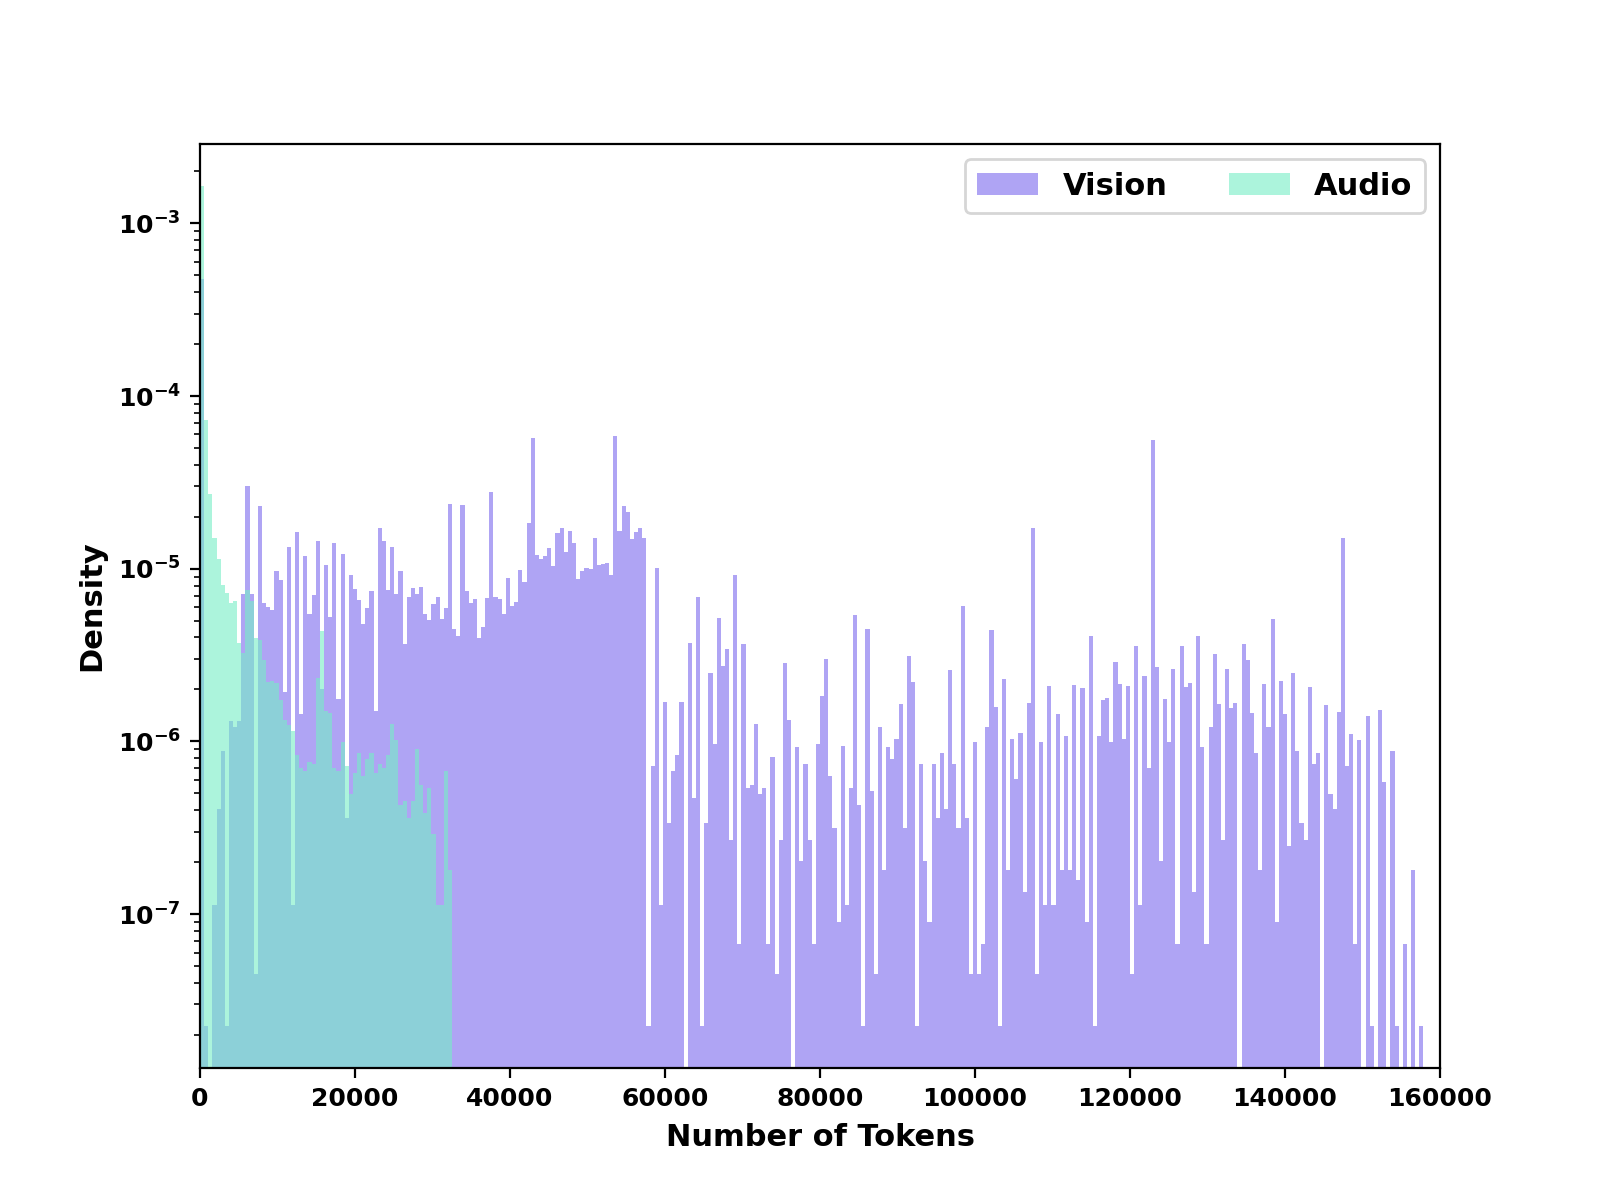
\includegraphics[width=\textwidth]{figs/data_distrubtion.png}
    \caption{The distribution of sequence token lengths across different modalities during the SFT stage.}
    \label{fig:data_distrubtion}
  \end{minipage}
\end{figure}

In multimodal scenarios, optimizing training performance is challenging due to the heterogeneity of both data and models. The challenge of data heterogeneity arises because the training data for \longcat includes speech, vision, and text, which show significant and dynamic differences in token distribution (Figure~\ref{fig:data_distrubtion}). 
Model heterogeneity is evident in the substantially different computational workloads across the three core components of \longcat: the vision encoder, the audio encoder, and the LLM decoder (Table~\ref{tab:modal_cost_dit}).
To address the aforementioned challenges, there are two primary optimization approaches. The first relies on Fully Sharded Data Parallelism (FSDP) (e.g., OrchMLLM~\citep{zheng2025orchestrate}, veOmni~\citep{ma2025veomni}), which reduces static memory consumption through parameter sharding, avoids pipeline parallelism (PP) bubbles caused by model heterogeneity, and mitigates data heterogeneity via data-parallel (DP) group balancing. However, for \longcat, the total number of model parameters is too large for this approach to be practical.

The second approach is to decouple multimodal models across different parallel dimensions. For example, DistTrain~\citep{zhang2025disttrain} mitigates model and data heterogeneity by separating model partitioning strategies and sorting data; PipeWeaver~\citep{xue2025pipeweaver} reduces PP bubbles caused by heterogeneity through fine-grained data partitioning and dynamic pipeline scheduling; and Optimus~\citep{feng2025optimus} separates the parallelization strategies for encoders and LLMs, scheduling encoder computations into the LLM’s idle periods to eliminate bubbles caused by model heterogeneity.
Building on the Optimus approach, we develop modality-decoupled parallelism (MDP), a simple yet effective multimodal training strategy. The core idea is to completely decouple the modality encoders and the LLM backbone at the distributed level, enabling independent scheduling and more efficient utilization of computational resources.

\subsubsection{Modality-Decoupled Parallelism}

\begin{figure}[t]
    \centering
    \includegraphics[width=\linewidth]{figs/mdp_v4.pdf}
    \caption{\textbf{Overview of modality-decoupled parallelism (MDP).} The modality encoders and the LLM backbone are fully decoupled at the distributed level, enabling independent scheduling and improved computational efficiency.}
    \label{fig:MDP}
\end{figure}

In our implementation, we co-locate the modality encoders and the LLM decoder. The modality encoders utilize Hybrid Sharding Data Parallelism (HSDP)\citep{zhao2023pytorchfsdpexperiencesscaling} to reduce static memory, and full activation recomputation is employed to reduce activation memory usage. The LLM decoder adopts a combined distributed strategy including pipeline parallelism (PP), ZeRO-1 data parallelism (DP), context parallelism (CP), and expert parallelism (EP). 
To simplify data mapping between modality encoders and the LLM decoder, we introduce an \textit{InnerDP} parallelism strategy, which further partitions modality data across all microbatches.
The DP rank of modality encoders corresponds one-to-one with the DP rank of the LLM decoder, and the size of the InnerDP dimension is the product of the PP and CP of the LLM decoder (i.e., $d_{inner\_dp}=d_{lm\_cp} \times d_{lm\_pp}$, $d_{world\_size}=d_{dp} \times d_{inner\_dp}$). As shown in Figure~\ref{fig:MDP}, the MDP execution timeline consists of four phases:

\textbf{Data Loading}: At the start of each training iteration, the rank with $inner\_dp=0$ fetches all micro-batches. Then it broadcasts the metadata of the data to the other ranks within the DP group. This mitigates I/O overhead and memory pressure. In this phase, all micro-batches are sorted by text data sequence length to ensure workload across DP groups remain similar, thereby reducing EP bubbles caused by workload imbalances.

\textbf{Modality Encoder Forward}: The BalanceData module first distributes the modality data from the $inner\_dp=0$ rank to the other $inner\_dp$ ranks. Then, the modality encoders on each rank compute the corresponding vision and audio embeddings. Finally, the ModalityBridge module aggregates these embeddings at the $inner\_dp=0$ rank, which are then passed as input to the LLM decoder.

\textbf{LLM Decoder Forward and Backward}: In this phase, modality embeddings are partitioned on the CP rank and fed into the LLM decoder for its forward and backward passes. The gradients of the vision and audio embeddings are then returned to the backward phase for the modality encoders. This design ensures the training efficiency of the LLM decoder, and also enables isolated optimization for modality encoders.

\textbf{Modality Encoder Backward}: The ModalityBridge module redistributes the modality embedding gradients from the LLM decoder to the other $inner\_dp$ ranks, and then the backward pass of the modality encoders is executed.

\subsubsection{ModalityBridge}

\begin{figure}
    \centering
    \includegraphics[width=1.0\linewidth]{figs/chunk_balance.pdf}
    % \caption{Overview of the chunk-based ModalityBridge. We show an example of the setting: num\_chunk=3, processing 4 microbatches (mbs) containing 8 images on 4 GPUs configured in DP=1, CP=2, and PP=2.}
    \caption{\textbf{Overview of the chunk-based ModalityBridge}. The example configuration with num\_chunk = 3, processing 4 microbatches of 8 images each across 4 GPUs (DP = 1, CP = 2, PP = 2)}
    \label{fig:chunk_balance}
\end{figure}

In MDP, the ModalityBridge serves as the communication layer between the multimodal encoders and the LLM decoder. 
It is responsible for transforming data organization formats to resolve discrepancies arising from the different parallelism strategies employed by the modality encoders and the LLM decoder. This process specifically involves handling modality embeddings during the forward phase and gradients during the backward phase.
However, when processing longer context length, significant memory pressure emerges as the $inner\_dp=0$ rank must read all micro-batches and perform gather and scatter operations on the modality embeddings and their gradients.
To address this challenge, we adopt chunk-based processing within ModalityBridge, which effectively alleviates the memory bottleneck while maintaining bitwise numerical consistency.
As illustrated in Figure~\ref{fig:chunk_balance}, this module comprises three core components:

\textbf{Embedding Redistribution}:
% Employs a two-stage chunk approach for data gather and scatter, decomposing the complete data transformation into $num\_chunk$ iterations. Each iteration consists of two stages:
% We employ a two-stage chunking approach for data gather and scatter, decomposing the complete data transformation into $num\_chunk$ iterations. Each iteration consists of two stages:
% (1) Aggregation of Inner-DP embeddings to the $inner\_dp=0$ rank;
% (2) CP partitioning, which splits along the $hidden\_size$ dimension to ensure uniform embedding distribution for memory balance, followed by scattering to respective CP ranks to reduce per-device memory.
% During each chunk process, the overall memory footprint exhibits a rise-then-fall pattern, significantly reducing the peak memory.
Employs a two-stage chunking approach for data gather and scatter, decomposing the complete data transformation into \(num\_chunk\) iterations. Each iteration consists of two stages:  
\begin{enumerate}
    \item \textbf{Aggregation:} Inner-DP embeddings are aggregated to the \(inner\_dp = 0\) rank.
    \item \textbf{CP partitioning:} The aggregated data is split along the \(hidden\_size\) dimension to ensure uniform embedding distribution and balanced memory usage, followed by scattering to the respective CP ranks to further reduce per-device memory consumption.
\end{enumerate}

During each chunking iteration, the overall memory footprint exhibits a rise-then-fall pattern, significantly lowering the peak memory usage.

% \textbf{Modality Embedding Storage}: Stores all gathered-then-scattered chunk data while maintaining global offset information for subsequent indexing.

% \textbf{Embedding Indexing}: Provides micro-batch-level embedding retrieval and gradient backpropagation in LLM forward/backward phases.

% Based on the three components, we accomplish the transformation of data format in different stages.
% In the forward phase, transformation is performed according to the two-stage chunk approach, while in the backward phase, \textit{Embedding Redistribution} executes the reverse process: gather gradients via CP gather, then scatter them to the corresponding $inner\_dp$ ranks according to global offset information for backward computation.
% Meanwhile, the chunk scheme reduces peak memory to $1/num\_chunk$ of the original, alleviating memory pressure while ensuring bitwise alignment.
\textbf{Modality Embedding Storage}: Stores all gathered-then-scattered chunk data while maintaining global offset information for subsequent indexing.

\textbf{Embedding Indexing}: Provides micro-batch-level embedding retrieval and gradient backpropagation during the LLM forward and backward phases.

Based on these three components, we accomplish the transformation of data formats across different stages. In the forward phase, the transformation is performed according to the two-stage chunking approach, while in the backward phase, \textit{Embedding Redistribution} executes the reverse process: gradients are first gathered via CP gather and then scattered to the corresponding \(inner\_dp\) ranks according to the global offset information for backward computation. Meanwhile, the chunking scheme reduces the peak memory usage to \(1/num\_chunk\) of the original, significantly alleviating memory pressure while ensuring bitwise numerical alignment.


\subsection{Performance Tuning}
Our overarching strategy is twofold: first, select a distributed configuration by profiling core operator efficiency; second, meet the configuration's memory budget via targeted memory optimizations. On the communication side, the shortcut architecture enables overlap between EP communication and computation within each micro-batch. In CPU-bound regimes, we employ fused operators to reduce kernel launch overhead and improve end-to-end throughput.
\subsubsection{Optimal Distributed Configuration}
In large-scale LLM pretraining, the efficiency of core operators is primarily constrained by the sequence length; increasing sequence length typically improves Model FLOPs Utilization (MFU). Accordingly, our system design increases the effective sequence length per EP rank to approach the operators' high-efficiency regime. Hardware-specific benchmarking results further indicate that reducing CP substantially improves the efficiency of the core operator, as shown in Figure~\ref{fig:mfu-ops}.
\begin{figure}
    \centering
    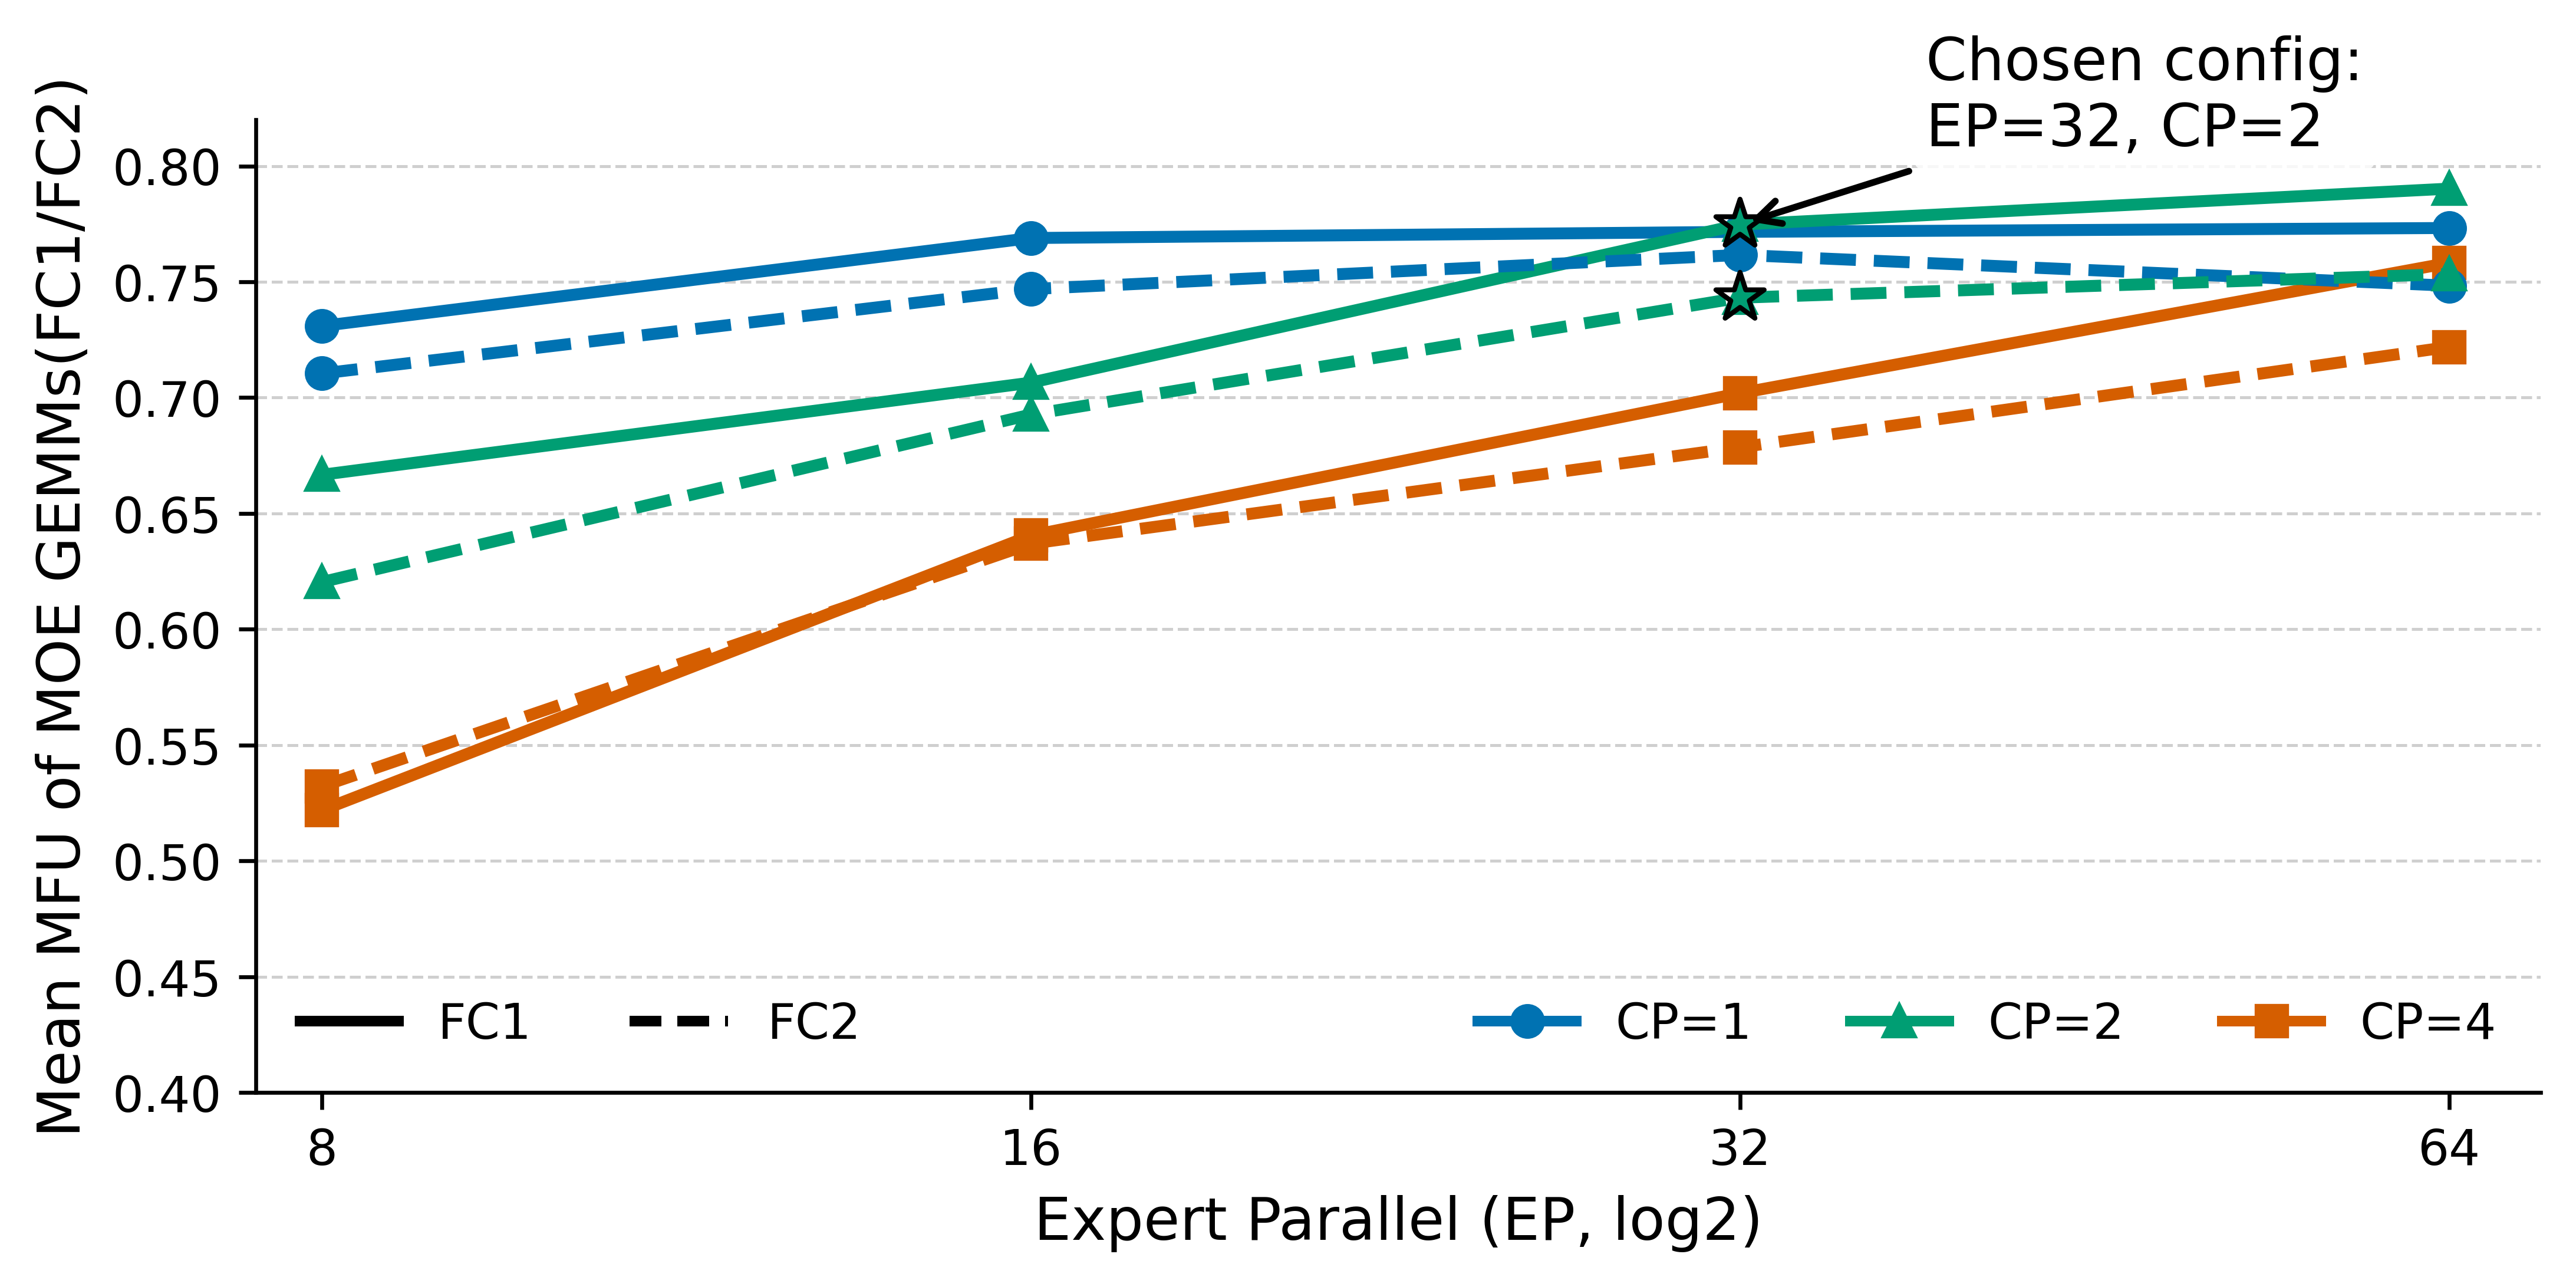
\includegraphics[width=0.8\linewidth]{figs/moe_mfu_ep_cp_log2.png}
    % \caption{Benchmark of MoE GEMMs with different CP/EP in 8K sequence.}
    \caption{Benchmark results of MoE GEMMs under different CP/EP configurations with an 8K sequence length.}
    \label{fig:mfu-ops}
\end{figure}
\subsubsection{Communication Optimizations}
Our training infra contains multiple compute-communication overlaps, mainly including shortcut-based EP overlap and point-to-point (P2P) overlap. We tune the number of streaming multiprocessors (SMs) assigned to communication and compute kernels for each scenario to maximize hardware utilization, and we use distinct P2P groups/streams so that inter-stage pipeline-parallel (PP) communication does not interfere across stages.

\subsubsection{Kernel Optimizations}
To optimize the training efficiency of MoE models, we maintain computational determinism while implementing kernel optimization and fusion along critical computational paths. Our technical contributions encompass the following areas:

\textbf{Optimized Grouped GEMM} 
% Our optimization strategies for Grouped GEMM achieve approximately 75\% MFU in evaluated scenarios. 
% (1) Dynamic SwapAB: WGMMA instruction is evaluated with N dimension varying from 8 to 256, while the M dimension is held constant at 64. We designed an optimized kernel where automatically do SwapAB to maximum WGMMA perfermance; (2) Configurable SM Usage: Grouped Gemm kernel allows configurable SM counts to avoid resource competition when overlapping with dispatch or combine communications; (3) FineTuning: TileShape, Pipeline Stage, and ClusterShape were meticulously tuned for the target workload to maximize hardware utilization and prevent register spilling; (4) Schedule and Pipeline Strategy: a swizzled block mapping schedule was adopted to improve L2 cache hit rates significantly. Also, a ping-pong mechanism was introduced during the backward pass, which overlaps WGMMA computation with the loading and storing of the weight gradient.
Our optimization strategies for Grouped GEMM achieve approximately 75\% MFU in the evaluated scenarios. 
(1) \textbf{Dynamic SwapAB:} The WGMMA instruction is evaluated with the $N$ dimension varying from 8 to 256, while the $M$ dimension is fixed at 64. 
We design an optimized kernel that automatically performs SwapAB operations to maximize WGMMA performance. 
(2) \textbf{Configurable SM Usage:} The Grouped GEMM kernel allows configurable SM counts to avoid resource contention when overlapping with dispatch or combined communication operations. 
(3) \textbf{Fine-Tuning:} \textit{TileShape}, \textit{PipelineStage}, and \textit{ClusterShape} are carefully tuned for the target workload to maximize hardware utilization and prevent register spilling. 
(4) \textbf{Scheduling and Pipeline Strategy:} A swizzled block mapping schedule is adopted to significantly improve L2 cache hit rates. 
In addition, a ping-pong mechanism is introduced during the backward pass to overlap WGMMA computation with the loading and storing of weight gradients.


\textbf{Fused Permute} 
% An efficient fused permute kernel is employed to rearrange tokens to be aligned with experts, and also fused some critical functionalities like: metadata computation for backward, token-drop at the cp-group. 
An efficient fused permute kernel is employed to rearrange tokens for expert alignment, while also integrating several critical functionalities, including metadata computation for the backward pass and token dropping within the CP group.


\textbf{Fused RoPE } 
% We fused RoPE into MLA prologue kernel, eliminating the overhead of intermediate data writing and reloading, which delivers a $3\times$ speedup compared to baseline.
We fuse RoPE into the MLA prologue kernel, eliminating the overhead of intermediate data writing and reloading, achieving a $3\times$ speedup compared to the baseline.


\textbf{Deterministic FA} 
% We used a semaphore-based synchronization scheme that ensuresd deterministic QK reduction in backward phase and outperformed the default deterministic version, which uses an extra temporary workspace. This can achieve approximately $0.8\times$ the performance of the non-deterministic version.
We employ a semaphore-based synchronization scheme that ensures deterministic QK reduction in the backward phase and outperforms the default deterministic implementation, which requires an additional temporary workspace. 
This approach achieves approximately $0.8\times$ the performance of the non-deterministic version.


\subsection{Memory Optimization Strategies}
% Without optimizations, the required memory of our target configuration is approximately 137 GB per device (Table~\ref{tab:mem-usage-naive}). With 80 GB devices and considering EP imbalance peaks, we constrain the theoretical footprint to about 72 GB.
Without optimization, the required memory for our target configuration is approximately 137~GB per device (Table~\ref{tab:mem-usage-naive}). 
Given 80~GB devices and accounting for EP imbalance peaks, we constrain the theoretical memory footprint to approximately 72~GB.

\begin{table}[htbp]
  \centering
    \caption{Naïve memory usage breakdown by component.}
    \label{tab:mem-usage-naive}
    \begin{tabular}{@{}l|rr@{}}
      \toprule
      \textbf{Component} & \textbf{Static (ZeRO-1, GB)} & \textbf{Dynamic (GB)} \\
      \midrule
      LLM                & 16.8  & 103.24 \\
      NCCL               & --    & 12.93  \\
      DeepEP             & --    & 0.45  \\
      Modality Encoders  & 3.6   & --     \\
      \midrule
      \textbf{Total} & \multicolumn{2}{c}{\textbf{137.02\,GB} (peak at non-pp0 stage)} \\
      \bottomrule
    \end{tabular}
\end{table}

We combine the techniques in Table~\ref{tab:mem-opts}: (i) a V-shaped PP schedule to bound concurrently alive activation micro-batches \citep{qi2024pipelineparallelismcontrollablememory}; (ii) selective recomputation for low-FLOP, high-activation operators such as SwiGLU and LayerNorm \citep{deepseekai2025deepseekv3technicalreport}; (iii) memory-efficient permute, which moves aggregation of routing probabilities and hidden states into SwiGLU to reduce MoE unpermute memory \citep{megatron-lm}; (iv) fine-grained SM budgeting for NCCL communicators to reduce NCCL memory; and (v) Hybrid-Sharding Data Parallel (HSDP) for the modality encoder to further reduce its static footprint \citep{paszke2019pytorch}.
To accommodate potential EP load imbalance, we implement \emph{dynamic expert recomputation}: when any rank is assigned too many tokens, we dynamically recompute its down-projection, freeing all MoE memory except the down-projection inputs on trigger. This prevents training crashes from expert imbalance while incurring only modest overhead.

\begin{table}[htbp]
  \centering
  \caption{Memory footprint under different optimization settings.}
  \label{tab:mem-opts}
  \begin{tabular}{@{}l|cccc@{}}
    \toprule
    \textbf{Setting} &
    \begin{tabular}[c]{@{}c@{}}\textbf{Static}\end{tabular} &
    \textbf{Dynamic(GB)} &
    \textbf{Others(GB)} &
    \textbf{Total(GB)} \\
    \midrule
    Baseline                         & 20.4  & 103.2 & 13.4 & 137.0 \\
    +HSDP for Modality Encoder       & 17.5  & 103.2 & 13.4 & 134.1  \\
    +Vhalf                           & 17.5  & 58.6  & 13.4 & 89.4   \\
    +Select Recompute                & 17.5  & 49.2  & 13.4 & 80.1   \\
    +Memory Efficient Permute        & 17.5  & 42.8  & 13.4 & 73.6   \\
    +NCCL Memory Optimization        & 17.5  & 42.8  & 8.9  & \textbf{69.1}   \\
    \bottomrule
  \end{tabular}
\end{table}

\subsection{Numerical Consistency}
Large language model pretraining is extremely resource-intensive, often requiring weeks and incurring millions in computational costs. Ensuring the correctness of the training framework is essential to avoid costly retraining due to implementation errors. 

In our framework, we enforce deterministic implementations for all computation, communication, and data flow, ensuring that every experiment is reproducible and maintains bitwise-aligned loss values.

For new features, we prioritize bit-aligned implementations to ensure numerical consistency. For example, features like \verb|fused_permute| and \verb|fused_swiglu| ensure bitwise-aligned loss whether they are enabled or not. 
Similarly, kernels like Grouped GEMM and Router GEMM employ a non Split-K implementation to preserve alignment across varying batch sizes or distributed settings.

For features where bit alignment is not feasible, we systematically analyze all sources of numerical deviation and mitigate their impact by benchmarking against the gold reference implementation during verification. For example, we identified and aligned the accumulation order in DeepEP and All2All EP strategies, thereby achieving bit-level consistency in loss values and verifying implementation correctness.


\section{Inference and Deployment} % @yulei
\label{sec7:infer}

\subsection{Decoupled Framework}
%Multimodal inference part consists of multiple modules, including encoders and decoders for each modality, as well as the LLM backbone. Each module has different optimal requirements for computational power, bandwidth, and network resources, making rational hardware resource allocation a key factor for performance.

%For the LLM backbone, the prefill stage is computation-intensive, while the decode stage is memory-intensive. We apply all existing LLM optimizations, including Prefill-Decode Disaggregation and mixing inference strategies.The encoder models for each modality (such as audio and video) are smaller in size and computation-intensive. Currently, the decoder modules primarily focus on audio and are also small, and they are memory-intensive.


% The multimodal inference framework comprises several modular components, including modality-specific encoders and decoders, as well as a large language model (LLM) backbone. Each of these modules exhibits distinct computational, bandwidth, and network resource requirements, rendering efficient and rational hardware resource allocation a critical determinant of overall system performance. The LLM backbone adopts the same architecture as LongCat-Flash, thereby employing identical inference optimization strategies, such as Prefill-Decode (PD) Disaggregation and Single Batch Overlap for ScMoE.

% Deploying modalities separately as Figure~\ref{fig:Decoupled_Framework} enables the use of specialized hardware accelerators tailored to each modality's unique requirements. The audio encoder/decoder, video encoder, and LLM backbone exhibit significant disparities in computational resources and operation types (e.g., compute-bound vs. memory-bound). Conventional hybrid deployment schemes suffer from suboptimal latency and throughput due to resource contention across modalities. While separated deployment introduces communication overhead, it ultimately achieves superior latency and throughput by eliminating cross-modal interference.

% 上面的内容精简为下面这一段：by wangyueqian
We propose a decoupled multimodal inference framework that separates modality-specific encoders/decoders and the LLM for optimized deployment. Each module is deployed on dedicated hardware and accelerators tailored to its computational characteristics, mitigating cross-modal resource contention. The optimizations of LLM deployment follow LongCat-Flash, including Prefill-Decode (PD) Disaggregation and Single Batch Overlap for ScMoE to improve inference efficiency. 
Compared with conventional hybrid deployment, this separation achieves lower latency and higher throughput despite minor communication overhead.


%There are roughly three types of multimodal inference deployment methods as Table ~\ref{tab:deployment-methods}.

% \begin{table}[htbp]
%   \renewcommand{\arraystretch}{1.5}
%   \centering
%   \caption{Multimodal inference deployment methods.}
%   \label{tab:deployment-methods}
%   \begin{tabular}{@{}p{5cm}p{5cm}p{5cm}@{}}
%     \toprule
%     \textbf{Methods} &
%     \textbf{Advantage} &
%     \textbf{Shortcoming} \\
%     \midrule
%     Single-instance, Multi-module Serial (Supports Asynchronous Pipeline) &
%     Simple to implement. &
%     Modules compete for GPU resources, leading to performance fluctuations. \\
%     \midrule
%     Single-instance with SM isolation for multiple module &
%     Strictly controls resource usage, reducing contention. &
%     Resource allocation needs to be dynamically adjusted based on request status, making implementation relatively complex. \\
%     \midrule
%     Modality-disaggregated deployment with heterogeneous devices partitioning &
%     Workflow is clearer, modules are decoupled, and each model can be deeply optimized accordingly; heterogeneous devices are fully utilized. &
%     Requires a complex scheduling system. \\
%     \bottomrule
%   \end{tabular}
% \end{table}


%We deploy different modules using different types of GPUs: the encoders and decoders for each modality are served on economical GPUs, while the LLM deployment strategy follows the LongCat approach. The number of replicas for each module can be configured individually based on module benchmarking results. This method maximizes computational resource utilization and minimizes interference between modules on the same machine(Figure~\ref{fig:Decoupled_Framework}). However, it also introduces transmission bottlenecks, especially when transferring long hidden states from the video encoder. To address this, we are also exploring homogeneous machine disaggregation combined with SM isolation. 

% \begin{figure}
%     \centering
%     \includegraphics[width=0.8\linewidth]{figs/Decoupled_Framework.png}
%     \caption{Decoupled Framework.}
%     \label{fig:Decoupled_Framework}
% \end{figure}


\subsection{Asynchronous Streaming Pipeline}
% 将整个inference流程集成到这里
\begin{figure}[t]
    \centering
    
\includegraphics[width=1.0\linewidth]{figs/streaming_pipeline.pdf}
    \caption{The asynchronous streaming pipeline for minimizing first packet latency.}
    \label{fig:streaming_pipeline}
\end{figure}

We design a highly efficient asynchronous streaming pipeline for model serving. As shown in Figure~\ref{fig:streaming_pipeline}, it consists of four sequentially linked and concurrently executed stages: VAD \& Frame Sampling, Audio-Visual Encoding, LLM Prefilling \& Decoding, and Audio Decoding. Each module supports incremental inference of streaming input and adaptive batching strategies, facilitating concurrent scheduling to reduce latency.

\textbf{Sparse-Dense Sampling Strategy} A voice activity detection (VAD) module is deployed to detect whether the user is speaking in real-time. When the user is speaking, densely sampled frames as well as the audio will be used as model input, facilitating a deeper analysis of the video content. Otherwise, only sparsely sampled frames are used to track the high-level overview of the video stream.

\textbf{Speculative Prefill-Decode Switching} Typically, the VAD model determines the end of a user turn by assessing whether the silence is longer than a predefined duration, referred to as the \textit{silent span} $[t_2, t_4]$. However, deferring the LLM state transition from prefill to decode until $t_4$ would incur substantial latency to the first packet. To overlap this latency with the latency of LLM decoding, we adopt a speculative prefill-decode switching strategy: The LLM starts decoding at an earlier speculative point $t_3$, reducing the latency from $t_3$ to $t_4$. If the user resumes speaking subsequently, a \textit{rollback} is triggered, wherein the LLM's generated content is discarded and the system reverts to the prefill state.

\textbf{Audio Delivery and Interruption} The audio will be delivered to the user once the VAD model explicitly detects the end of a turn, which is marked as $t_4$ in the figure, even if the first packet of audio response is generated earlier. However, should a user interrupt the audio generation at $t_5$, the process is immediately terminated. Consequently, the token sequence from the LLM is truncated at the nearest natural breakpoint, such as the most recent punctuation mark.

% by qianyulei
% 在使用LongCat-Omni构建全模态实时交互的产品时，每个请求数据包，我们采用1秒音频对应2帧视频的配比关系。由于采用了流式Prefill，系统不需要等待用户完成语音输入才进行计算。在用户完成语音输入之后，系统使用600-700ms的窗口进行输入判停。由于判停窗口和Prefill计算耗时overlap，在判停结束之后只需要额外的不到100ms，用户即可接收到模型返回的输出。基于上述异步pipeline，用户可以在结束输入之后接收到系统毫秒级的返回，实现实时全模态交互。

In our implementation, each request data packet from the user side consists of 1 second of audio and 2 corresponding video frames. Using the streaming prefill strategy, each request packet can be immediately prefilled, eliminating the need to wait until the user's turn to finish before initiating computation. By overlapping the VAD endpoint detection ($600\sim700 ms$) and the prefill process, users can receive the model response within $100ms$ after the endpoint detection. This asynchronous pipeline enables real-time omni-modal interaction.


% First, a voice activity detection (VAD) module detects the start and end times of user speech. We use sparsely-sampled frames as input when the user is not speaking ($[0, t_1]$ and $[t_3, t_5]$), and densely-sampled frames as well as the audio as input when the user is speaking ($[t_1, t_3]$ and after $t_5$). Then, audio-visual input are asynchronously encoded by the audio and video encoder, and sent to LLM for pre-filling.
% Pre-filling proceeds until the VAD module detects an end of speech pre-stop, when the LLM switches to the decode mode and begins generating text and audio output tokens, which are then sent to the audio decoder to generate audio and return to the user.

% There are two notable details: First, the audio output is only sent to the user after the VAD model detects a stop. If a stop is not subsequently detected (i.e., the continuous silence time after the pre-stop does not reach a threshold), the LLM will discard its generated tokens and revert to the pre-filling mode. Second, if a user interruption occurs during the audio decoding process, this process will be immediately terminated, the tokens decoded by the LLM will be rolled back to an appropriate position (e.g., the position of the most recent punctuation mark), and the tokens generated after that point will be discarded.

% Multimodal real-time interaction has become a mainstream development need, with streaming processing being the core element of real-time interaction. A single voice/video input can reach over 10k tokens, and waiting for a one-time inference can lead to end-to-end multi-module first package return times that reach the level of seconds. To better provide real-time performance, the entire input is split into multiple segments for streaming input. After each module processes a segment, it is transmitted downstream for pipeline processing, which effectively reduces processing latency.

% To achieve an asynchronous pipeline, the algorithm structure needs to reduce the use of full attention in some module. The main approach is to ensure dependencies only on the most recent k inputs in the encoder/decoder parts while utilizing full attention in the LLM part.

% In terms of engineering implementation, each module needs to support streaming and adopt different batching strategies according to its characteristics, while the scheduler coordinates the overall streaming state(Figure~\ref{fig:Pipeline}).

% For scenarios involving multi-segment splits, a typical example is the user's input being segmented. The initially inputted part first enters the encoder and LLM for prefill calculations, using the time of user speech to hide the encode and prefill time, thereby avoiding high initial response latency due to overly long requests. We call this feature "thinking while listening/watching."

% Output is also streamed, as each inferred codec token by the LLM decode is sent to the decoder module to generate a segment of audio, using audio playback time to mask decoder time.

% \begin{figure}
%     \centering
%     \includegraphics[width=0.8\linewidth]{figs/Pipeline.png}
%     \caption{Asynchronous Streaming Pipeline.}
%     \label{fig:Pipeline}
% \end{figure}

% \subsection{Streaming State Machine}
% 和下一个subsection合并，一起写整个inference过程

% \begin{figure}
%     \centering
%     \includegraphics[width=0.8\linewidth]{figs/Streaming_State_Machine.png}
%     \caption{Streaming State Machine for Encoder/Decoder and LLM.}
%     \label{fig:Streaming_State_Machine}
% \end{figure}
% Due to the presence of streaming and interactions, it essentially involves multi-turn request, requiring the scheduler to be aware of the session state. Requests need to be scheduled to the corresponding instance of a submodule, and each submodule also needs to support saving the historical state of requests.

% Typically, with streaming, the usual state is executing a decode after multiple prefill operations. Beyond that, to cope with interactive scenarios, there are two additional states:
% \begin{enumerate}
% \item Interruption: This feature means the model's output is interrupted by the user during the decode process. At this point, it is necessary to terminate the decode and transition the state to the next round of prefill.

% \item Rollback: Based on business scenario requirements, revert to a specified token output position. One scenario involves rollback because the inference speed is faster than the audio playback speed, so after interruption, it's necessary to roll back the part that was inferred but not output to the user. Another scenario involves retracting the useless prefill information from the previous round of inference.
% \end{enumerate}

% \begin{figure}[t]
%     \centering
%     \includegraphics[width=1.0\linewidth]{figs/deploy-fig1.pdf}
%     \caption{Real-Time Scheduler Flow Diagram.}
%     \label{fig:deploy_pipeline_flow}
% \end{figure}

% \begin{figure}[t]
%     \centering
%     \includegraphics[width=1.0\linewidth]{figs/deploy-fig2.pdf}
%     \caption{Real-Time Scheduler Sequence Diagram.}
%     \label{fig:deploy_pipeline_sequence}
% \end{figure}

% Thus, a state machine mechanism needs to be designed to maintain and transition states for real-time interactive scenarios as Figure~\ref{fig:Streaming_State_Machine}:
% \begin{enumerate}
% \item For the encoder/decoder part, since the model only needs to focus on the current round request, we only pay attention to a part of historical data, taking it out from the state pool to splice with the current data for inference.

% \item For the LLM part, complete historical data is required to support full attention operations. This involves multi-turn data state transitions and needs to support multiple functions like partial prefill/decode/interruption/rollback, which involves reading/adding/deleting the KV cache as well as operations such as termination in continue batching.
% \end{enumerate}


% \subsection{Real-Time Full-Duplex System}
% In real-time conversational interaction, the system functionally supports full-modality (streaming audio + video + text) input, as well as voice + text or only text output, while also enabling capabilities like FunctionCall and RAG. Technically, it employs a pipeline architecture to orchestrate various AI sub-services, including full-duplex turn detection, audio/video encoding, model inference, and audio decoding. The end-to-end interaction latency on the server side can reach approximately 613 ms, shown in Figure~\ref{fig:deploy_pipeline_flow} and Figure~\ref{fig:deploy_pipeline_sequence}.
% Core Highlights:
% \begin{enumerate}
% \item multimodal Support:
% Handles various frame types (text, image, audio, etc.), enabling rich media processing.
% \item Flexibility and Extensibility:
% Bidirectional pipeline architecture allows arbitrary orchestration of parallel/primary-secondary pipelines.The modular design supports dynamic pipeline reconfiguration for custom workflows.
% \item High Efficiency and Ultra-Low Latency:
% Frame-level processing: Data flows in small chunks (frames), ensuring real-time processing granularity.Asynchronous execution: Parallel and master-slave async modes minimize end-to-end latency. Simultaneous viewing, listening, and thinking—an ultimate interactive latency experience.
% \end{enumerate}

% by wangyueqian
% 我的理解：
% 1. VAD/EOS模块负责将时间分为两类：用户在说话的时间段 和用户不在说话的时间段
% 2. 对于用户在说话的时间段，我们将image embedding和audio embedding交替输入LLM
% 3. 对于用户不在说话的时间段，我们只输入image embedding到LLM。而且这些image embedding都放在assistant回复的后面
% ⬆️ 如果语音生成完了，而不是被用户打断的，会怎么样？

% In real-time, full-duplex audio-visual interaction, the system functionally supports several modality inputs, including streaming audio, video and text, as well as flexible output modalities such as voice + text or text-only responses. It also enables advanced capabilities such as \textit{FunctionCall} and \textit{RAG}. From a technical perspective, the system adopts a pipeline-based architecture to orchestrate various sub-services, including turn detection, audio/video encoding, LLM decoder model inference, and audio decoding.
% With extensive tests, the end-to-end interaction latency on the server side of the LongCat-Flash-Omni model can reach approximately 613~ms, as shown in Figure~\ref{fig:deploy_pipeline_flow} and Figure~\ref{fig:deploy_pipeline_sequence}, with the following core highlights:
% \begin{enumerate}
%     \item \textbf{multimodal Support:}  
%     The system processes diverse input frame types (e.g., text, image, video and audio), enabling rich multimodal interactions and comprehensive media understanding.

%     \item \textbf{Flexibility and Extensibility:}  
%     A bidirectional pipeline architecture supports arbitrary orchestration of parallel or primary-secondary pipelines. The modular design allows dynamic reconfiguration, enabling customized workflows tailored to specific application scenarios.

%     \item \textbf{High Efficiency:}  
%     \textit{Frame-level processing:} Data is streamed in small chunks (frames), ensuring fine-grained, real-time processing.  
%     \textit{Asynchronous execution:} Parallel and master-slave asynchronous modes minimize end-to-end latency.  
%     This enables simultaneous “watching, listening, and reasoning,” delivering an exceptionally low-latency interactive experience.
% \end{enumerate}



\section{Evaluation} % fengjiao, liusongxiang
\label{sec5:eval}

In this section, we conduct comprehensive evaluations of \longcat, compare it with various proprietary and open-source multimodal models, including vision understanding, audio comprehension, text understanding and generation, cross-modality understanding, and audio-visual interaction.

\subsection{Vision Capability Evaluation}
% compare with sota omni-model and open-source best model (qwen3-vl, mimo-vl-chat, glm4.5v)

\begin{table}[htbp]
    \caption{Evaluation of image understanding. Values marked with * are sourced from public reports. As GPT-4o does not support image grounding, we do not report its results on RefCOCO and ScreenSpot-v2.}
    \centering
    \resizebox{1.0\textwidth}{!}{
        \begin{tabular}{l|cccccc|cl}
            \toprule
            Benchmark & \begin{tabular}[c]{@{}c@{}}\textbf{LongCat-Flash-Omni} \\ Instruct\end{tabular} & \begin{tabular}[c]{@{}c@{}}Gemini-2.5-Pro \\ {\small ThinkingBudget128}\end{tabular} & \begin{tabular}[c]{@{}c@{}}Gemini-2.5-Flash \\ {\small non-thinking}\end{tabular} & \begin{tabular}[c]{@{}c@{}}Qwen3-Omni \\ Instruct\end{tabular} & Seed-1.6 & \begin{tabular}[c]{@{}c@{}}GPT-4o \\ 1120\end{tabular} & \begin{tabular}[c]{@{}c@{}}Qwen3-VL \\ {\small 235B-A22B-Instruct}\end{tabular} & \begin{tabular}[c]{@{}c@{}}Qwen2.5-VL \\ {\small 72B-Instruct}\end{tabular} \\ 
            \midrule
            \multicolumn{9}{c}{\textbf{General}} \\
            \midrule
            MMBench-EN$_{\text{test}}$ &87.5 & 89.8 & 89.3 & 86.8 & 88.5 & 83.7 &88.3 & 88.6* \\
            MMBench-ZH$_{\text{test}}$ &88.7 & 89.2 & 88.5 & 86.4 & 83.8  & 82.8 &89.8 & 87.9* \\
            RealWorldQA                & 74.8 & 76.0 & 73.9 & 72.9 & 74.5 & 74.1 &79.3* & 75.7* \\
            % HallusionBench             & 51.9 & 60.9 & 57.70  & 59.7  & 56.0 & 53.6 &63.2* & 55.2* \\
            MMStar                     & 70.9 & 78.5* & 75.5 & 68.5* & 71.5 & 63.2 &78.4* & 68.2 \\
            % VStar                      & 73.3 & 80.1 & 74.35  & 86.9 & 79.6 & 64.9 &85.3 & 86.9 \\
            % VlmsAreBlind               & 57.9? & 80.1 & 74.67 & 61.3 & 83.5 & 56.1 &75.9 & 66.9 \\
            % MME-RealWorld-EN         
            \midrule
            \multicolumn{9}{c}{\textbf{STEM \& Reasoning}} \\
            \midrule
            % MathVision$_{\text{test}}$ & 50.4 & 66.0* & 58.68 & 56.3* & 49.5 & 32.4 &66.5* & 38.1* \\
            MathVista$_{\text{mini}}$  & 77.9 & 77.7* & 77.1 & 75.9  & 78.7 & 62.8  &84.9* & 74.8* \\
            MMMU$_{\text{val}}$        & 70.7 & 80.9* & 76.3 & 69.1* & 74.9 & 69.4 &78.7* & 70.2* \\  
            % MMMU-pro                   & 55.1 & 71.2* & 67.46 & 57.0* & 61.8 & 54.1 &68.1* & 51.1* \\  
            MMVet                      & 69.0 & 80.7 & 79.5 & 68.9 & 74.4 & 76.6 &75.9 & 74.5 \\
            \midrule
            \multicolumn{9}{c}{\textbf{Multi-Image}} \\
            \midrule
            BLINK                      & 63.1 & 70.0* & 65.7 & 56.1 & 65.0 & 65.5 &70.7* & 60.1 \\
            MuirBench                  & 77.1 & 74.0* & 73.7 & 62.1 & 74.6 & 70.5 &72.8* & 70.7* \\  
            Mantis                     & 84.8 & 83.9  & 83.4 & 80.7 & 81.1 & 79.3 &79.7 & 82.0 \\
            \midrule
            \multicolumn{9}{c}{\textbf{Text Recognition \& Chart/Document Understanding}} \\
            \midrule
            % AI2D$_{\text{test}}$  & 80.6 & 90.0* & 82.6 & 85.2*  & 80.8 & 84.4* & 85.2 & 88.7* \\
            ChartQA               & 87.6 & 71.7 & 77.6 & 86.8*  & 82.4 & 74.5  & 89.2 & 89.5* \\
            % CharXiv\_RQ/DQ        &47.4/83.6?  & 66.3/89.5 &60.0/87.7 & 45.4/78.6   & 52.7/85.5 & 49.1/83.2 & 54.2/89.0 & 49.7/87.4* \\
            DocVQA                & 91.8 & 94.0* & 93.6*  & 95.7   & 94.3 & 80.9  & 94.6 & 96.4* \\
            OCRBench              & 84.9 & 87.2*  & 85.6 & 85.5   & 85.6 & 82.3  & 91.2 & 88.5 \\
            OmniDocBench$_{\text{EN/ZH}}$↓   & 22.8/29.0 & 31.9/24.5 & 22.8/32.9 & 28.4/40.5 & 22.0/27.6  & 25.9/37.7 & 13.6/17.5 & 22.6/32.4* \\
            \midrule
            \multicolumn{9}{c}{\textbf{Grounding \& Counting}} \\
            \midrule
            RefCOCO-avg        & 93.9 & 80.2 & 74.8  & 91.6  & 87.5  & -     & 88.2 & 92.3 \\
            % RefCOCO-avg        & 92.3 & 75.4  & 71.9  & 89.3  & 80.2  & -     & 87.1 & 90.3 \\
            CountBench             & 92.4 & 91.0* & 78.6  & 90.0* & 94.1  & 85.6* & 94.3 & 93.6* \\
            \midrule
            \multicolumn{9}{c}{\textbf{Graphical User Interface (GUI)}} \\
            \midrule
            VisualWebBench       & 78.7 & 81.1  & 73.5  & 79.3  & 81.1 & 77.1 & 80.8  & 82.3* \\
            ScreenSpot-v2        & 91.2 & 75.8  & 63.9  & 94.7  & 91.7 & -    & 93.4  & 92.9 \\
            AndroidControl   & 91.2 & 79.2  & 79.1  & 90.5  & 84.6 & 65.2 & 90.0  & 93.7* \\
            % AndroidControl$_{\text{high}}$  & 75.6 & 60.8  & 55.5  & 70.8  & 55.2 & 41.7 & 74.1 & 67.4* \\
            \bottomrule
        \end{tabular}
    }
    \label{tab:eval_image_und}
\end{table}

In this section, we compare LongCat-Flash-Omni with omni-models (Gemini-2.5-Pro\citep{comanici2025gemini}, GPT-4o\footnote{\url{https://openai.com/index/hello-gpt-4o}}, Seed-1.6\footnote{\url{https://seed.bytedance.com/en/seed1_6}}, and Qwen3-Omni\citep{xu2025qwen3}) and vision language models (Qwen3-VL\citep{yang2025qwen3} and Qwen2.5-VL-72B\citep{Qwen2.5-VL}) without thinking mode.

Note that GPT-4o and Seed-1.6 only provide a vision understanding API. Therefore, we evaluate them solely on visual capabilities. To ensure a fair comparison with instruct model, we follow the evaluation setting used in Qwen3-VL benchmark, limiting Gemini-2.5-Pro’s thinking budget to 128 tokens. All models are evaluated under their official configurations.

\subsubsection{Image-to-Text Evaluation}
We conduct a comprehensive evaluation of image understanding across six key dimensions, leveraging a diverse suite of benchmarks:
\begin{itemize}
    % \item \textbf{General Domains}: MMBench\citep{liu2024mmbench}, RealWorldQA\citep{realworldqa}, HallusionBench\citep{hallusionbench}, MMStar\citep{mmstar}, VStar, and VlmAreBlind\citep{vlms2024blind}; + MME-RealWorld-EN
    \item \textbf{General Domains}: MMBench~\citep{liu2024mmbench}, RealWorldQA~\citep{realworldqa}, and MMStar~\citep{mmstar}.
    
    % \item \textbf{STEM \& Reasoning}: MathVision\citep{wang2024mathvision}, MathVista\citep{lu2024mathvista}, MMMU\textsubscript{val}\citep{yue2023mmmu}, MMMU-pro\citep{yue2025mmmupro}, and MMVet\citep{yu2024mmvet}.
    \item \textbf{STEM \& Reasoning}: MathVista~\citep{lu2024mathvista}, MMMU\textsubscript{val}~\citep{yue2023mmmu}, and MMVet~\citep{yu2024mmvet}.
    
    \item \textbf{Multi-Image}: BLINK~\citep{fu2024blink}, MuirBench~\citep{wang2024muirbench}, and Mantis~\citep{jiang2024mantis}.
    
    \item \textbf{Text Recognition \& Document Understanding}: ChartQA~\citep{masry2022chartqa}, DocVQA~\citep{mathew2021docvqa}, and OCRBench~\citep{liu2024ocrbench}, OmniDocBench\textsubscript{EN/ZH}~\citep{ouyang2024omnidocbench}.
    
    \item \textbf{Grounding \& Counting}: RefCOCO, RefCOCO+~\citep{kazemzadeh-2014-refcoco} (averaged in RefCOCO-avg), and CountBench\citep{paiss2023countbench}.
    
    \item \textbf{Graphical User Interface (GUI)}: VisualWebBench~\citep{liu2024visualwebbench}, ScreenSpot-v2~\citep{wu2024atlas}, and AndroidControl~\citep{li2024androidcontrol}.
\end{itemize}

Results on image understanding benchmarks are summarized in Table~\ref{tab:eval_image_und}. Overall, LongCat-Flash-Omni achieves performance comparable to Gemini-2.5-Flash, while outperforming the open-sourced Qwen3-Omni. Its advantage is particularly pronounced on multi-image tasks, which benefit from the model’s training on high-quality interleaved image-text, multi-image data and video datasets.

\subsubsection{Video-to-Text Evaluation}
To assess the capability of video understanding, we consider three dimensions as below:
\begin{itemize}
    \item \textbf{Short Video}: MVBench~\citep{li2024mvbench}, NextQA~\citep{xiao2021nextqa}, and TempCompass~\citep{liu2024tempcompass}.
    \item \textbf{Long Video}: VideoMME~\citep{fu2024videomme} and LongVideoBench~\citep{wu2024longvideobench}.
    %\item \textbf{Streaming Video}: OVBench~\citep{huang2025ovbench}.
    \item \textbf{STEM \& Reasoning}: MMVU~\citep{zhao2025mmvu}, and Video-MMMU~\citep{hu2025videommmu}.
    % \item \textbf{Video Grounding}: Charades-STA~\citep{charades-sta}.
\end{itemize}
% VideoMME offers an evaluation of audio-visual understanding, so we provide the results for both scenarios: with audio (referred to as VideoMME(w/ audio)) and without audio (referred to as VideoMME(w/o audio)), while both using the w/o subset setting. All video benchmarks adopt a maximum 32K-token for consistent benchmarking.
% VideoMME provides an evaluation of audio-visual understanding; therefore, we report results for two scenarios: with audio (denoted as ``VideoMME w/ audio'') and without audio (denoted as ``VideoMME w/o audio''), both under the ``w/o subtitle'' setting.
We evaluate audio-visual understanding on VideoMME under the no-subtitle protocol (w/o sub), and report results for two conditions: with audio (“VideoMME w/ audio”) and without audio (“VideoMME w/o audio”).

% As Gemini does not support video without audio, we only report VideoMME with audio for Gemini. 
As the Gemini models do not provide official evaluation entries for videos without audio, we report only the ``VideoMME w/ audio'' results.
All video benchmarks are evaluated using a maximum context length of 32K tokens to ensure consistent comparison.
% As illustrated in Table~\ref{tab:eval_video_und}, LongCat-Flash-Omni shows a competitive performance to Gemini-2.5-pro. Especially for long video, LongCat-Flash-Omni reaches 77.99 in VideoMME and closes to Gemini-2.5-pro in LongVideoBench. This gain is attributed to the advanced video strategy (including dynamic frame sampling and hierarchical token aggregation), as well as the long context support by the efficient backbone. For short video, LongCat-Flash-Omni achieves significantly outperforming Gemini-2.5-pro and Qwen-3-Omni in MVBench, and remains a performance gap to vision-only model (i.e. Qwen3-VL-235B-A22B-Instruct), demonstrating a competitive vision understanding strength.

% As illustrated in Table~\ref{tab:eval_video_und}, LongCat-Flash-Omni exhibits state-of-the-art performance on video-to-text tasks. Specifically, LongCat-Flash-Omni outperforms the compared models by a large margin on short video understanding, demonstrating its superior video understanding performance. On long video tasks, LongCat-Flash-Omni is comparable to Gemini-2.5-Pro and Qwen3-VL. Especially in VideoMME, LongCat-Flash-Omni performances the best among omni-modal models. This achievement can be attributed to its advanced video processing strategy (dynamic frame sampling and hierarchical token aggregation) and the long context support by its efficient backbone.
As shown in Table~\ref{tab:eval_video_und}, LongCat-Flash-Omni achieves state-of-the-art performance on video-to-text tasks. Specifically, it surpasses all compared models by a significant margin on short video understanding, demonstrating superior video comprehension capabilities. On long video tasks, LongCat-Flash-Omni demonstrates performance on par with leading models such as Gemini-2.5-Pro and Qwen3-VL. Notably, in the VideoMME benchmark, it achieves the best performance among omni-modal models. This can be attributed to a combination of an advanced video processing strategy—using dynamic frame sampling and hierarchical token aggregation—and the strong long-context modeling capacity afforded by its efficient backbone.
% TODO: 等streaming和video grounding成绩出来之后再决定怎么写

\begin{table}[htbp]
    \caption{Evaluation of video understanding. Values marked with * are sourced from public reports.}
    \centering
    \resizebox{1.0\textwidth}{!}{
        \begin{tabular}{l|cccccc|cl}
            \toprule
            Benchmark & \begin{tabular}[c]{@{}c@{}}\textbf{LongCat-Flash-Omni} \\ Instruct\end{tabular} & \begin{tabular}[c]{@{}c@{}}Gemini-2.5-Pro \\ {\small ThinkingBudget128}\end{tabular} & \begin{tabular}[c]{@{}c@{}}Gemini-2.5-Flash \\ {\small non-thinking}\end{tabular} & \begin{tabular}[c]{@{}c@{}}Qwen3-Omni \\ Instruct\end{tabular} & Seed-1.6 & \begin{tabular}[c]{@{}c@{}}GPT-4o \\ 1120\end{tabular} & \begin{tabular}[c]{@{}c@{}}Qwen3-VL \\ {\small 235B-A22B-Instruct}\end{tabular} & \begin{tabular}[c]{@{}c@{}}Qwen2.5-VL \\ {\small 72B-Instruct}\end{tabular} \\ 
            \midrule
            \multicolumn{9}{c}{\textbf{Short Video}} \\
            \midrule
            MVBench           & 75.2  & 66.4  & 63.0 & 69.3* & 68.4 & 62.1  & 71.3 & 70.4* \\
            % MVBench           & 75.2  & 66.4  & 63.0 & 65.7 (69.3*) & 68.4 & 62.1  & 71.3 & 70.4* \\
            NextQA            & 86.2 & 84.2 & 81.4 & 82.4 & 84.1 & 79.7  & 81.3 & 82.3 \\
            % VSIBench          & -     & 29.9  & 29.09 & 59.7  & 42.4 & 44.46  & 59.0(62.6*) & 39.73 \\
            TempCompass       & 82.2 & 80.8  & 80.2 & 73.5  & 79.4 & 76.4  & 80.5 & 74.8* \\
            \midrule
            \multicolumn{9}{c}{\textbf{Long Video}} \\
            \midrule
            VideoMME w/o audio & 76.2 & -     & -     & 70.5* & 75.2 & 73.2  & 79.2* & 73.3* \\
            % VideoMME(w/o audio) & 76.2 & -     & -     & 71.7 (70.5*) & 75.2 & 73.2  & 74.8(79.2*) & 73.3* \\
            VideoMME w/ audio & 78.2     & 80.6* & 78.5 & 73.0 & - & -  & - & - \\
            LongVideoBench    & 69.3 & 69.4  & 66.4 & 65.4 & 64.8 & 63.9  & - & 60.7* \\
            \midrule
            %\multicolumn{9}{c}{\textbf{Streaming Video}} \\
            %\midrule
            %OVBench           &  58.8  & 48.8  & 42.3 & - & 48.3 & 49.7  & 53.2 & 51.1 \\ %(74.8*) \\
            %\midrule
            \multicolumn{9}{c}{\textbf{STEM \& Reasoning}} \\
            \midrule
            MMVU              & 67.1 & 75.6  & 72.4 & 62.4 & 67.3 & 67.4  & 69.3 & 62.9* \\
            Video-MMMU        & 67.5 & 79.4* & 76.6 & 60.3 & 75.4 & 68.0  & 73.7 & 59.3 \\
            % MMVU              & 67.1 & 75.6  & 72.4 & 62.4 & 67.3 & 67.4  & 69.3 & 64.7(62.9*) \\            
            % Video-MMMU        & 67.5 & 83.0 (79.4*) & 76.6 & 60.3 & 75.4 & 68.0  & 73.7 & 59.3 \\
            % \midrule
            % \multicolumn{9}{c}{\textbf{Video Grounding}} \\
            % \midrule
            % Charades-STA      & -     & 64.8* & -     & 38.67 & 55.95 & 35.7* & 64.8* & 50.9* \\
            \bottomrule
        \end{tabular}
    }
    \label{tab:eval_video_und}
\end{table}


\subsection{Audio Capability Evaluation}
\label{sec:audio-eval}

\subsubsection{Base Model Evaluation}

To systematically assess the audio capability of the base models produced in the pre-training stages (i.e., stage-1, stage-2, stage-3, and stage-4), we conduct evaluations with respect to the following three aspects: automatic speech recognition (ASR), text-to-speech (TTS), and speech continuation.
For ASR evaluation, we employ the SPEECHIO\_ASR\_ZH00002 (speechio02)~\footnote{\url{https://github.com/SpeechColab/Leaderboard}} to test Chinese speech recognition, while utilizing the LibriSpeech \citep{panayotov2015librispeech} for English speech recognition assessment. 
The evaluation results are presented in Table~\ref{tab:base_asr_tts_eval}. Remarkably, our model demonstrates competitive performance across these benchmark datasets, despite relying on discretized audio features.

\begin{table}[h!]
\centering
\caption{ASR and TTS performance of base models during the pre-training stages. Word error rate (WER) (for English) or character error rate (CER) (for Chinese) in percentage are reported.}
\resizebox{0.8\textwidth}{!}{
\begin{tabular}{lccccc}
\toprule
\textbf{Base Model} & \multicolumn{3}{c}{\textbf{ASR}} & \multicolumn{2}{c}{\textbf{TTS}} \\
\cmidrule(lr){2-4} \cmidrule(lr){5-6}
& \textbf{SpeechIO02↓}
 & \begin{tabular}[c]{@{}c@{}}\textbf{LibriSpeech} \\ \textbf{test-clean↓} \end{tabular} & \begin{tabular}[c]{@{}c@{}}\textbf{LibriSpeech} \\ \textbf{test-other↓} \end{tabular} & \textbf{SpeechIO02↓} & \textbf{LibriSpeech↓} \\
\midrule
Stage-1 & 2.93 & 1.98 & 3.96 & 4.12 & 4.72 \\
Stage-2 & 3.18 & 2.11 & 4.59 & 2.16 & 8.64 \\
Stage-3 & 3.01 & 1.93 & 3.74 & 2.53 & 3.68 \\
Stage-4 (32K) & 3.49 & 2.30 & 4.00 & 1.73 & 5.99 \\
Stage-4 (128K) & 3.46 & 2.12 & 4.15 & 2.62 & 7.38 \\
\bottomrule
\end{tabular}
}
\label{tab:base_asr_tts_eval}
\end{table}

The TTS evaluation framework uses text samples from the speechio02 and LibriSpeech~\citep{panayotov2015librispeech} test-clean/other datasets as input sources. The model uses discrete semantic-acoustic tokens as speech prompts, conducting speech token generation with text input as teacher-forcing guidance. The output speech tokens are reconstructed into waveform by the audio decoder. We compute the word error rate (WER) (for English) or character error rate (CER) (for Chinese) between transcription of the generated speech produced by a robust ASR system and the original input text as the measure for the evaluation. The results are shown in the right part of Table~\ref{tab:base_asr_tts_eval}. We observe that the base models are capable of generating robust speech from textual input, providing a solid foundation for speech output in spoken and audio-visual interaction modes.
% we can see that the base models are capable of generating robust speech from input text, providing foundational speech-out capability in the spoken or audio-visual interaction mode.

To evaluate speech continuation capabilities, we develope a specialized test set comprising $1,200$ synthesized speech samples derived from text data from the CMMLU \citep{li2023cmmlu} benchmark.
The assessment requires the model to generate appropriate responses to multiple-choice questions based on provided speech input. For text outputs, we directly measure response accuracy, while speech outputs undergo ASR transcription before accuracy evaluation. The evaluation protocol employs a 1-shot learning approach, with detailed results presented in Table~\ref{tab:base_speech_cmmlu}. 
Our analysis reveals that the base models in different stage perform well in in-context speech continuation evaluation and there is only a negligible performance disparity between text and speech output.

\begin{table}[h!]
\centering
\caption{Speech continuation performance of base models across pre-training stages. Accuracy is reported as a percentage.}
\resizebox{0.5\textwidth}{!}{
\begin{tabular}{lcc}
\toprule
\textbf{Base Model} & \multicolumn{2}{c}{\textbf{Speech Continuation (CMMLU)↑}} \\
\cmidrule(lr){2-3}
& \textbf{Audio In Text Out}
 & \textbf{Audio In Audio Out} \\
\midrule
Stage-1 & 88.80 & 84.80 \\
Stage-2 & 89.60 & 84.80 \\
Stage-3 & 92.80 & 92.00 \\
Stage-4 (32K) & 91.20 & 91.20 \\
Stage-4 (128K) & 90.40 & 90.40 \\
\bottomrule
\end{tabular}
}
\label{tab:base_speech_cmmlu}
\end{table}


\subsubsection{Instruct Model Evaluation}

We conduct comprehensive evaluation of the audio capabilities of \longcat, covering speech recognition and translation, audio understanding and audio-to-text chat.


\textbf{Speech Recognition and Translation}

\begin{table}[t] %[htbp]
    \caption{Automatic speech recognition (ASR) and speech-to-text translation (S2TT) evaluation results.}
    \centering
    \resizebox{1.0\textwidth}{!}{
\begin{tabular}{c|cccccc}
\toprule
Benchmark & \begin{tabular}[c]{@{}c@{}}\textbf{LongCat-Flash-Omni} \\ Instruct\end{tabular} & \begin{tabular}[c]{@{}c@{}}Gemini-2.5-Pro \\ {\small ThinkingBudget128}\end{tabular} & GPT-4o-Audio & \begin{tabular}[c]{@{}c@{}}Qwen3-Omni \\ Instruct\end{tabular} & Kimi-Audio & Step-Audio-2-mini  \\ 
\midrule
\multicolumn{7}{c}{\textbf{ASR}} \\
\midrule
\begin{tabular}[c]{@{}c@{}}\textbf{LibriSpeech} \\ test-clean | test-other\end{tabular} & 1.57 | 4.01 & 1.74 | 3.80 & 30.00 | 41.83 & 1.22 | 2.48 & 1.28 | 2.42 & 1.33 | 2.86 \\
\textbf{AISHELL-1} & 0.63 & 3.11 & 34.81  & 0.84  & 0.60 & 0.78 \\
\textbf{AISHELL-2} & 2.78 & 5.24 & 77.73 & 2.34 & 2.56 & 2.16 \\
\begin{tabular}[c]{@{}c@{}}\textbf{Fleurs} \\ zh | en \end{tabular} & 3.99 | 5.02 & 2.24 | 4.77 & 3.91 | 5.56 & 2.20 | 2.72 & 2.69 | 4.44 & 2.53 | 3.05 \\
\begin{tabular}[c]{@{}c@{}}\textbf{CommonVoice 15} \\ zh | en \end{tabular} & 4.98 | 13.59 & 47.30 | 49.86 & 42.83 | 23.88 & 4.31 | 6.05 & 8.46 | 7.92 & 5.00 | 6.75 \\
\begin{tabular}[c]{@{}c@{}}\textbf{WenetSpeech} \\ test-meeting | test-net \end{tabular} & 6.69 | 6.09 & 136.13 | 32.82 & 54.35 | 67.90 & 5.89 | 4.69 & 6.28 | 5.37 & 4.87 | 4.82 \\
\midrule
\multicolumn{7}{c}{\textbf{S2TT (BLEU)}} \\
\midrule
\textbf{CoVost2 en$\rightarrow$zh} & 47.23 & 41.94 & 29.32 & 48.72  & - & 49.12 \\
\textbf{CoVost2 zh$\rightarrow$en} & 27.32 & 25.38 & 16.01 & 21.51  & - & 29.47 \\

\bottomrule
\end{tabular}
}
\label{tab:eval_asr_ast}
\end{table}


\begin{table}[t]
    \caption{Evaluation results of audio understanding.}
    \centering
    \resizebox{1.0\textwidth}{!}{
\begin{tabular}{c|cccccc}
\toprule
Benchmark & \begin{tabular}[c]{@{}c@{}}\textbf{LongCat-Flash-Omni} \\ Instruct\end{tabular} & \begin{tabular}[c]{@{}c@{}}Gemini-2.5-Pro \\ {\small ThinkingBudget128}\end{tabular} & GPT-4o-Audio & \begin{tabular}[c]{@{}c@{}}Qwen3-Omni \\ Instruct\end{tabular} & Kimi-Audio & Step-Audio-2-mini  \\ 
% \midrule
% \multicolumn{6}{c}{\textbf{Audio Analysis}} \\
\midrule
\textbf{MMAU} & 75.90 & 72.80 & 68.40 & 77.50  & 65.20 & 73.20 \\
\textbf{VocalSound} & 92.76 & 89.45 & 82.37  & 91.60  & 94.85 & 87.58 \\
\textbf{TUT2017} & 65.43 & 33.15 & 20.74 & 40.74  & 65.25 & 30.67 \\
\textbf{ClothoAQA} & 72.83 & 69.67 & 61.87  & 75.16  & 72.21 & 68.39 \\
\textbf{Nonspeech7k} & 93.79 & 87.59 & 72.28 & 80.83  & 93.93 & 73.24 \\
\textbf{CochlScene} & 70.02 & 45.34 & 34.94 & 43.03  & 80.42 & 44.58 \\
\textbf{MELD} & 54.60 & 46.74 & 39.00 & 50.80  & 59.13 & 31.44 \\

\bottomrule
\end{tabular}
}
\label{tab:eval_audio_understanding}
\end{table}

For ASR evaluation, as presented in Table~\ref{tab:eval_asr_ast}, we use LibriSpeech~\citep{panayotov2015librispeech}, AISHELL-1~\citep{bu2017aishell}, AISHELL-2~\citep{du2018aishell}, FLEURS~\citep{conneau2023fleurs}, CommonVoice15~\citep{ardila2019common}, and WenetSpeech~\citep{zhang2022wenetspeech} as benchmarks. We observe that \longcat consistently achieves superior performance compared to other competitors, including Gemini-2.5-Pro~\citep{comanici2025gemini}, GPT-4o-Audio, Qwen3-Omni-Instruct~\citep{xu2025qwen3}, Kimi-Audio~\citep{ding2025kimi}, and Step-Audio-2-mini~\citep{wu2025step}.
For speech-to-text translation (S2TT) evaluation, we adopt CoVost2~\citep{wang2021covost}. As shown in Table~\ref{tab:eval_asr_ast}, \longcat exhibits strong S2TT capabilities among all models\footnote{Kimi-audio defaults to ASR rather than executing the requested translation task.}. Taken together, the speech recognition and translation results demonstrate that LongCat-Flash-Omni possesses robust and comprehensive fundamental speech understanding capabilities.

\textbf{Audio Understanding}
As an omni-modal model, \longcat can effectively function as a native audio understanding model when vision input is not provided. We conduct a comprehensive evaluation of \longcat across a diverse set of audio comprehension tasks, including music, sound events, and speech understanding. Specifically, we use MMAU~\citep{sakshi2024mmau}, VocalSound~\citep{gong_vocalsound}, TUT2017~\citep{Mesaros2016_EUSIPCO}, ClothoAQA~\citep{lipping2022clotho}, Nonspeech7k~\citep{rashid2023nonspeech7k}, CochlScene~\citep{jeong2022cochlscene}, and MELD~\citep{poria2018meld} as benchmarks.
The results, presented in Table~\ref{tab:eval_audio_understanding}, show that \longcat consistently outperforms most competing models across all evaluated dimensions, and achieves state-of-the-art performance in several benchmarks. These findings highlight that \longcat possesses advanced capabilities in understanding a wide spectrum of general and complex acoustic information, going well beyond conventional speech recognition.

\textbf{Audio-to-Text Chat} We evaluate the ability of \longcat to engage in text-based conversations driven by audio instructions using the OpenAudioBench~\citep{li2025baichuan} and VoiceBench~\citep{chen2024voicebench} benchmarks. These benchmarks assess a wide range of capabilities, including world knowledge, domain-specific understanding, instruction following, and reasoning.
To ensure standardized and reproducible results, we employ the official evaluation code provided by the benchmark authors. The results, presented in Table~\ref{tab:eval_a2t_chat}, show that \longcat achieves strong performance across all benchmark subsets, reaching state-of-the-art results in several cases. Overall, these results demonstrate \longcat’s superior ability to conduct audio-driven conversations and perform complex reasoning tasks.

% \textbf{Spoken Dialogue} In addition to supporting streaming audio-visual interaction, \longcat can inherently function as a spoken interaction model. To evaluate its speech-in-speech-out conversational capabilities, we construct a proprietary benchmark named MT-CLUE-Voice.
% While existing open-source evaluation frameworks, such as AirBench~\citep{yang2024air} and SD-Eval~\citep{ao2024sd}, have advanced the assessment of audio understanding capabilities, they fall short in effectively evaluating interactive voice dialogue functionality. Drawing inspiration from the GPT-4o evaluation framework, we design a comprehensive evaluation methodology by:
% (1) collecting and filtering text-based evaluation data to remove code snippets, tabular data, advanced mathematical content, and other elements unsuitable for voice dialogue;
% (2) organizing the curated data into six specialized categories — Idiom Explanation (Idiom), Content Generation (Content), Advice Seeking (Advice), Elementary Mathematics (Math), Translation (Trans.), and Classical Text Interpretation (Ancient); and
% (3) constructing dedicated evaluation test sets for each category.
% To create audio instruction inputs, we employ a TTS model to convert text queries into speech, and we use GPT-4o-mini as the scoring engine to assess the quality of the generated spoken responses.
% The analysis of evaluation results presented in Table~\ref{tab:eval_aiao} shows that LongCat-Flash-Omni outperforms Qwen3-Omni-Instruct in speech-based conversational tasks.


% speech-to-speech tasks, we implement a specialized evaluation protocol where text evaluation data is first converted to speech using our proprietary TTS engine, then processed by the model to generate both speech and text outputs. 
% The evaluation methodology differs for each output modality: text responses are assessed directly, while speech outputs are first transcribed into text through our in-house ASR system before undergoing evaluation.
% The evaluation of voice dialogue capabilities remains a significant challenge in the research community. 

% The evaluation process involved: (1) synthesizing text-based questions into audio format using advanced TTS technology; (2) feeding the audio inputs to the model and capturing both textual and audio responses; (3) employing GPT-4o-mini as the scoring engine for comprehensive evaluation. For voice-output assessment, we implemented an additional processing step where audio responses are first transcribed into text using state-of-the-art ASR systems before being subjected to text-based evaluation metrics.

% 我们从中文开源文本评测集中（belle、deepctrl）筛选出一些特定任务数据，任务包括翻译、内容生成、成语解释、古文解释、寻求建议、数学应用题。然后通过文本改写转换成TTS友好的形式，然后通过TTS合成语音用作模型的输入音频。我们利用gpt-4o-mini对模型的输出进行打分来评价模型的语音对话能力，每个子任务都会得到一个分数，然后取各个子任务的平均分用作最终的语音对话能力得分。

% Analysis of the evaluation results in Tables\,\ref{tab:aiao} and \ref{tab:aito} reveals that LongCat-Flash-Omni achieves superior performance over GLM4-Voice in both voice and text output evaluations following its two stages of fine-tuning process, demonstrating enhanced capabilities across most test categories. 
% A critical finding is the substantial performance gap between voice-based and text-based evaluations, which can be attributed to three primary factors: (1) inherent limitations and recognition errors of the ASR system, (2) quality variations in speech synthesis, and (3) processing challenges with non-standard text formats.

% Considering the fundamental architecture of these models, where text serves as the primary guidance signal for dialogue generation, text-based evaluation inherently represents the theoretical maximum performance ceiling for voice dialogue capabilities. 
% Although the indirect evaluation methodology through ASR transcription introduces potential recognition errors that may affect absolute scores, the comparative performance trends and relative score distributions across models remain valid indicators of voice dialogue competence and speech generation fidelity.

% \begin{figure}[h]
%   \centering
%   \includegraphics[width=0.6\textwidth]{figs/audio_eval.png}
%   \caption{Audio Evaluation Framework}
%   \label{fig:audio_eval}
% \end{figure}



\begin{table}[t] %[htbp]
    \caption{Evaluation results of audio-to-text chat.}
    \centering
    \resizebox{1.0\textwidth}{!}{
\begin{tabular}{c|cccccc}
\toprule
Benchmark & \begin{tabular}[c]{@{}c@{}}\textbf{LongCat-Flash-Omni} \\ Instruct\end{tabular} & \begin{tabular}[c]{@{}c@{}}Gemini-2.5-Pro \\ {\small ThinkingBudget128}\end{tabular} & GPT-4o-Audio & \begin{tabular}[c]{@{}c@{}}Qwen3-Omni \\ Instruct\end{tabular} & Kimi-Audio & Step-Audio-2-mini  \\ 
\midrule
\multicolumn{7}{c}{\textbf{OpenAudioBench}} \\
\midrule
% \textbf{AlpacaEval}     & 75.43 & 76.58 & 81.61 & 85.43  & 75.73 & 53.92 \\
\textbf{LlamaQuestions} & 83.33 & 83.00 & 86.30 & 83.30  & 79.33 & 69.70 \\
\textbf{ReasoningQA}    & 79.71 & 80.30 & 68.71 & 84.16  & 58.02 & 55.64 \\
\textbf{TriviaQA}       & 86.20 & 90.20 & 76.00 & 75.90  & 62.10 & 45.30 \\
\textbf{Webquestions}   & 76.00 & 80.90 & 81.20 & 75.20  & 70.20 & 54.40 \\
\textbf{AlpacaEval}     & 75.43 & 76.58 & 81.61 & 85.43  & 75.73 & 53.92 \\

\midrule
\multicolumn{7}{c}{\textbf{VoiceBench}} \\
\midrule
\textbf{AlpacaEval} & 4.94  & 4.70  & 4.73  & 4.74  & 4.46  & 3.84 \\
\textbf{CommonEval} & 4.32  & 4.11  & 4.37  & 4.54  & 3.97  & 3.19 \\
\textbf{OpenBookQA} & 93.41 & 95.16 & 87.90 & 89.70 & 83.52 & 72.97 \\
\textbf{SDQA}       & 82.46 & 83.54 & 90.10 & 76.90 & 63.12 & 44.85 \\
\textbf{MMSU}       & 81.95 & 88.32 & 78.90 & 69.00 & 62.17 & 52.00 \\
\textbf{AdvBench}   & 100   & 97.69 & 99.23 & 99.30 & 100   & 97.00 \\
\textbf{IFEval}     & 77.99 & 77.83 & 66.81 & 77.80 & 61.10 & 29.80 \\
\bottomrule
\end{tabular}
}
\label{tab:eval_a2t_chat}
\end{table}

% During Stage 5, we maintained the LLM in a frozen state while exclusively training the audio encoder, effectively transforming the system into an audio comprehension model. 
% The performance evaluation of this configuration is comprehensively presented in Table\,\ref{tab:stage5_res}. 
% It is important to note that our streaming audio encoder architecture inherently incurs some performance degradation compared to non-streaming alternatives. 
% Furthermore, to preserve the LLM's textual capabilities, we intentionally kept the LLM parameters fixed during this stage, which consequently established a performance ceiling.

% We conceptualize this stage as serving two primary objectives: (1) aligning continuous speech representations with the LLM's semantic space, and (2) establishing foundational audio comprehension capabilities that can be further refined during subsequent supervised fine-tuning stages. 
% Empirical evidence suggests that the current stage's performance is adequate to facilitate robust audio understanding. 
% However, we acknowledge that limited training data represents a significant constraint on performance, and we are actively developing optimization strategies to enhance task-specific performance in future iterations.


\subsection{Text Capability Evaluation}
\subsubsection{Base Model Evaluation}
We compare the LongCat-Flash-Omni Base model (i.e., after pre-training stage 5) with other strong text-based models across the following core capabilities and corresponding benchmarks.: (1) \textbf{General Tasks:} MMLU~\citep{hendrycks2021measuringmassivemultitasklanguage}, MMLU-Pro~\citep{wang2024mmluprorobustchallengingmultitask}, C-Eval~\citep{huang2023ceval}, and CMMLU~\citep{li2023cmmlu}. (2) \textbf{Reasoning Tasks:} GPQA~\citep{rein2023gpqagraduatelevelgoogleproofqa}, SuperGPQA~\citep{pteam2025supergpqascalingllmevaluation}, BBH~\citep{BBH}, PIQA~\citep{piqa}, DROP~\citep{drop}, CLUEWSC~\citep{clue}, and WinoGrande~\citep{winogrande}. (3) \textbf{Math Tasks:} GSM8K~\citep{cobbe2021gsm8k}, MATH~\citep{mathbenchmark}. (4) \textbf{Coding Tasks:} MBPP+~\citep{humanevalmbppplus}, HumanEval+~\citep{humanevalmbppplus}, MultiPL-E~\citep{cassano2022multiplescalableextensibleapproach}, and CRUXEval~\citep{gu2024cruxevalbenchmarkcodereasoning}. We follow the same evaluation protocol as in \citep{meituan2025longcat_flash_chat} to ensure maximum fairness.

% As shown in Table~\ref{tab:text_eval_base}, 
% The reasons for these enhancements—whether they stem from extended pre-training time, the inclusion of additional speech data, or a combination of both—remain an open question for future research.
% Furthermore, we compare the results before and after annealing, revealing that the model achieves significant improvements in evaluation metrics after annealing training.
Table~\ref{tab:text_eval_base} presents the evaluation results across diverse benchmarks. 
LongCat-Flash-Omni Base model achieves performance on par with state-of-the-art base models despite its compact active/total parameter size. Furthermore, our model demonstrates no degradation in text capabilities after extensive training with multimodal data, indicating the effectiveness of our training strategy.

% 将longcat-flash-omni和longcat-flash移动到前面
\begin{table}[htbp]
    \caption{Comparison between LongCat-Flash-Omni and other base models on text-only benchmarks. Values marked with * are sourced from public reports.}
    \centering
    \resizebox{0.8\textwidth}{!}{
    \begin{tabular}{l|c|ccc}
        \toprule
        Benchmark & \begin{tabular}[c]{@{}c@{}}\textbf{\longcat} \\ Base\end{tabular}  & \begin{tabular}[c]{@{}c@{}}LongCat-Flash \\ Base\end{tabular} & \begin{tabular}[c]{@{}c@{}}DeepSeek-V3.1 \\ Base\end{tabular} &  \begin{tabular}[c]{@{}c@{}}Kimi-K2 \\ Base\end{tabular} \\ 
        \midrule
        Architecture & MoE & MoE  & MoE  & MoE  \\
        \# Total Params & 560B & 560B & 671B & 1043B \\
        \# Activated Params & 27B & 27B & 37B & 32B \\
        \midrule
        \multicolumn{5}{c}{\textbf{General Domains}} \\
        \midrule
        MMLU $_{\text{(acc)}}$  & 86.81  & 87.05 & 87.46  & 87.47 \\
        MMLU-Pro $_{\text{(acc)}}$ & 69.05  & 70.32 & 59.29  & 68.36 \\
        CEval $_{\text{(acc)}}$ & 87.95  & 87.73 & 89.33  & 91.24 \\
        CMMLU $_{\text{(acc)}}$ & 87.14  & 87.19 & 88.21  & 90.35  \\
        \midrule
        \multicolumn{5}{c}{\textbf{General Reasoning}} \\
        \midrule
        GPQA $_{\text{(acc)}}$ & 51.76  & 51.09  & 47.16 & 45.89  \\
        SuperGPQA $_{\text{(acc)}}$ & 54.71  & 54.19 & -  & 44.70* \\
        BBH $_{\text{(acc)}}$ & 90.42 & 90.54 & 89.46 & 89.19 \\
        DROP $_{\text{(f1)}}$ & 80.75  & 78.39  & 80.74 & 69.81 \\
        PIQA $_{\text{(acc)}}$ & 92.27  & 92.33 & 93.00 & 95.10 \\
        WinoGrande $_{\text{(acc)}}$ & 85.95  & 85.08 & 83.50 & 82.87 \\
        CLUEWSC $_{\text{(acc)}}$ & 91.45  & 91.12 & 88.16 & 76.32 \\

        \midrule
        \multicolumn{5}{c}{\textbf{Mathematical Reasoning}} \\
        \midrule

        GSM8K $_{\text{(acc)}}$ & 93.10  & 92.19 & 92.22 & 92.27 \\
        MATH $_{\text{(acc)}}$ &  66.80 & 64.82 & 61.56 & 66.74 \\
        \midrule
        \multicolumn{5}{c}{\textbf{Coding}} \\
        \midrule
        MBPP+ $_{\text{(pass@1)}}$ & 76.46  & 77.25 & 59.26 & 80.49 \\
        HumanEval+ $_{\text{(pass@1)}}$ & 69.51  & 65.85  & 67.07  & 69.84 \\
        MultiPL-E $_{\text{(pass@1)}}$ & 70.76  & 69.25 & 62.00  & 59.22 \\
        CRUXEval-I $_{\text{(pass@1)}}$ & 71.88  & 71.63 & 65.87 & 65.87 \\
        CRUXEval-O $_{\text{(pass@1)}}$ & 73.50  & 75.88 & 71.25 & 68.75 \\
        \bottomrule
    \end{tabular}
    }
    \label{tab:text_eval_base}
\end{table}

% 将longcat-flash-omni和longcat-flash移动到前面
\begin{table*}[t] 
     \centering 
     \caption{Evaluation results of frontier chat/instruct models. Values marked with * are sourced from other public reports. Note that DeepSeek-V3.1, Qwen3-235B-A22B, Gemini2.5-Flash, and Claude Sonnet-4 are evaluated under their non-thinking mode.}
     \label{tab:text_eval_results} 
     \resizebox{\textwidth}{!}{ 
     \begin{tabular}{l|c|c|ccc|ccc} 
         \toprule 
         Benchmark & \begin{tabular}[c]{@{}c@{}}\textbf{LongCat-Flash-Omni} \\ Instruct \end{tabular} & \begin{tabular}[c]{@{}c@{}}LongCat-Flash \\ \end{tabular} & \begin{tabular}[c]{@{}c@{}}DeepSeek \\ V3.1\end{tabular} & \begin{tabular}[c]{@{}c@{}}Qwen3 \\ MoE-2507\end{tabular} & \begin{tabular}[c]{@{}c@{}}Kimi-K2 \\ \end{tabular} & GPT-4.1 & \begin{tabular}[c]{@{}c@{}}Claude \\ Sonnet-4\end{tabular} & \begin{tabular}[c]{@{}c@{}}Gemini-2.5 \\ -Flash\end{tabular} \\ 
         \midrule 
         
Architecture & MoE & MoE & MoE & MoE & MoE & - & - & - \\ 
         \# Total Params & 560B & 560B & 671B & 235B & 1043B & - & - & - \\ 
         \# Activated Params & 27B & 27B & 37B & 22B & 32B & - & - & - \\ 
         \midrule 
         \multicolumn{9}{c}{\textbf{General Domains}} \\ 
  
        \midrule 
         MMLU $_{\text{(acc)}}$ & 90.30 & 89.71 & 90.96 & 90.23 & 89.86 & 89.64 & 91.75 & 86.33 \\ 
         MMLU-Pro $_{\text{(acc)}}$ & 82.73 & 82.68  & 84.45 & 84.83 & 82.06 & 81.72 & 83.74 & 81.95 \\ 
         % ArenaHard-V2 & 45.20 & 86.50 & 84.10 & 88.20 & 85.70  & 61.50 & 62.10 & 77.00 \\ 
         CEval $_{\text{(acc)}}$ & 91.68 & 90.44 & 89.21 & 92.70 & 91.26 & 79.53 & 86.63 & 78.78 \\ 
         CMMLU $_{\text{(acc)}}$ & 89.39 & 84.34 & 88.04 & 88.14 & 89.66 & 77.65 & 86.51 & 78.30 \\ 
         \midrule 
         \multicolumn{9}{c}{\textbf{Instruction Following}} \\ 
        
 \midrule 
         IFEval $_{\text{(acc)}}$ & 82.44 & 89.65 & 86.69 & 88.54 & 88.91 & 85.58 & 88.35 & 83.92 \\ 
         COLLIE $_{\text{(acc)}}$ & 45.69 & 57.10 & 43.80 & 49.71 & 56.34 & 50.00 & 51.22 & 48.60 \\ 
         Meeseeks-zh $_{\text{(acc)}}$ & 39.05 & 43.03 & 33.83 & 35.32 & 42.79 & 41.54 & 35.07 & 34.84 \\ 
         \midrule 
       
  \multicolumn{9}{c}{\textbf{Mathematical Reasoning}} \\ 
         \midrule 
         MATH500 $_{\text{(acc)}}$ & 97.60 & 96.40   & 96.08 & 98.80 & 97.60 & 90.60 & 93.80 & 98.40\\ 
         AIME24 $_{\text{(avg@10)}}$ & 72.92 &  70.42  & 66.30* & 81.67 & 69.60* & 47.00 & 47.00 & 79.67 \\ 
         % AIME25 $_{\text{(avg@10)}}$  & 61.77 & 61.25  & 49.27 & 68.33 & 50.66 & 32.00 & 37.00 & 67.33 \\ 
     BeyondAIME $_{\text{(avg@10)}}$ & 47.40 & 43.00 & 36.50 & 57.60 & 36.60 & 22.10 & 20.50 & 44.20 \\ 
         \midrule 
         \multicolumn{9}{c}{\textbf{General Reasoning}} \\ 
         \midrule 
         GPQA-diamond $_{\text{(acc)}}$ & 74.41 & 73.23 & 74.90* & 77.43 & 75.76 & 67.68 & 70.71 & 80.30 \\ 
         DROP $_{\text{(f1)}}$ & 83.53 & 79.06  & 84.19 & 78.57 & 89.04 & 66.94 & 73.06 & 45.03 \\ 
         ZebraLogic $_{\text{(acc)}}$ & 86.00 & 89.30  & 85.30 & 94.22 & 89.11 & 56.30* & 80.10 & 57.00 \\ 
         GraphWalks-128K $_{\text{(precision)}}$ & 56.00 & 51.05  & 73.54 & 80.72 & 47.50 & 85.02 & 80.57 & 64.83 \\ 
         \midrule 
         \multicolumn{9}{c}{\textbf{Coding}} \\ 
         \midrule 
   
         LiveCodeBench $_{\text{(pass@1)}}$ & 52.64 & 48.02 & 56.40*  & 46.48 & 46.70 & 39.21 & 45.59 & 39.65 \\ 
         Humaneval+ $_{\text{(pass@1)}}$ & 90.85 & 88.41  & 92.68 & 94.51 & 85.98 & 93.29 & 94.51 & 87.80 \\ 
         MBPP+ $_{\text{(pass@1)}}$ & 80.16 & 79.63  & 79.89 & 79.89 & 81.75 & 79.37 & 80.16 & 76.19 \\ 
         \bottomrule 
     \end{tabular}
     } 
 \end{table*}


\subsubsection{Instruct Model Evaluation}

A comprehensive and rigorous text capability evaluation of the \longcat Instruct model is performed, covering diverse capability dimensions, including general domains, instruction following, mathematical reasoning,
general reasoning, and coding, using the following benchmarks:
\begin{itemize}
    \item \textbf{General Domains:} MMLU~\citep{hendrycks2021measuringmassivemultitasklanguage}, MMLU-Pro~\citep{wang2024mmluprorobustchallengingmultitask}, CEval~\citep{huang2023ceval}, and CMMLU~\citep{li2023cmmlu}.
    \item \textbf{Instruction Following:} IFEval~\citep{zhou2023ifeval}, COLLIE~\citep{yao2024collie}, and Meeseeks~\citep{meeseeks}, Meeseeks evaluates models' instruction-following capabilities in multi-turn scenarios through an iterative feedback framework that simulates realistic human-LLM interactions, enabling models to self-correct based on turn-specific failures and better reflect real-world usage patterns.
    \item \textbf{Mathematical Reasoning:}  MATH500~\citep{math500}, AIME24~\citep{AIME24}, and BeyondAIME~\citep{bytedance_seed_2025_beyondaime}.
    \item \textbf{General Reasoning:}  GPQA-diamond~\citep{rein2023gpqagraduatelevelgoogleproofqa}, DROP~\citep{drop}, ZebraLogic~\citep{lin2025zebralogic}, and GraphWalks~\citep{graphwalks}.
    \item \textbf{Coding:}  Humaneval+~\citep{humanevalmbppplus}, MBPP+~\citep{humanevalmbppplus}, and LiveCodeBench (2024.08-2025.05)~\citep{jain2025livecodebench}.
    % SWE-Bench-Verified~\citep{jimenez2024swebench}, and TerminalBench~\citep{tbench_2025}.
    % \item \textbf{Agentic Tool Use:}  $\tau^2$-Bench~\citep{tau2-bench}, AceBench~\citep{chen2025acebench} and VitaBench~\citep{meituan2025longcat_flash_chat}.
\end{itemize}


\begin{table*}
    \caption{Evaluation of cross-modality understanding. We use an internally corrected version of OmniBench, as the publicly released version contains scoring deficiencies.}
    \centering
    \resizebox{1.0\textwidth}{!}{
        \begin{tabular}{l|ccc|cc}
            \toprule    
            Benchmark & \begin{tabular}[c]{@{}c@{}} \textbf{LongCat-Flash-Omni} \\ Instruct\end{tabular} &  \begin{tabular}[c]{@{}c@{}} Gemini-2.5-Pro \\ {\small ThinkingBudget128}\end{tabular} & \begin{tabular}[c]{@{}c@{}} Gemini-2.5-Flash \\ non-thinking \end{tabular} & \begin{tabular}[c]{@{}c@{}}Qwen3-Omni \\ Instruct \end{tabular} & \begin{tabular}[c]{@{}c@{}} Qwen2.5-Omni \\ Instruct\end{tabular} \\ 
            \midrule    
            OmniBench  & 61.38  & 66.80 & 54.99       & 58.41 & 48.16  \\
            WorldSense & 60.89  & 63.96 & 58.72       & 52.01 & 46.69 \\
            DailyOmni  & 82.38  & 80.61 & 80.78       & 69.33 & 47.45 \\
            UNO-Bench  & 49.90  & 64.48 & 54.30       & 42.10 & 32.60 \\
            % UNO-Bench\small{-MC}  & 49.90  & 64.48 & 54.30       & 42.10 & 32.60 \\
            % UNO-Bench\small{-MO}  & 42.68  & 57.32 & 47.08       & 37.08 & 27.72 \\
            \bottomrule
        \end{tabular}
        }
    \label{tab:eval_cross_modal_und}
\end{table*}



We compare \longcat with some representative text chat models including DeepSeek-V3.1~\citep{deepseekai2025deepseekv3technicalreport}, Qwen3-235B-A22B (2507 version)~\citep{yang2025qwen3}, Kimi-K2~\citep{Kimi_K2_web_doc}, GPT-4.1~\citep{gpt4.1}, Claude Sonnet-4~\citep{claude4}, Gemini2.5-Flash~\citep{comanici2025gemini} and LongCat-Flash\citep{meituan2025longcat_flash_chat}. For closed-source models, we conduct evaluations through their official APIs. For models supporting both thinking and non-thinking modes (Qwen3-235B-A22B, Gemini-2.5-Flash, and Claude Sonnet-4), we explicitly configure these models to operate in non-thinking mode for a fair comparison.
The evaluation results are presented in Table~\ref{tab:text_eval_results}. the comprehensive evaluation demonstrates that \longcat maintains superior text capability, with consistently leading performance in different domains. Compared with LongCat-Flash, whose early base model serves as the foundation for LongCat-Flash-Omni, the latter not only exhibits no degradation in text capabilities but even achieves superior performance in certain domains. This highlights the effectiveness of our training strategy and underscores the potential synergy among different modalities in omni-modal model training.


% \begin{table}[htbp]
% \centering
% \caption{The Audio-In-Audio-Out Dialogue Evaluation (TO BE UPDATED)}
% \begin{tabular}{cccccccc}
% \toprule
% \multirow{2}{*}{Model} & \multicolumn{6}{c}{Voice  Dialogue Evalution (Audio-In-Audio-Out)↑} & \multirow{2}{*}{Avg.} \\ \cline{2-7}
%                        & Idiom  & Content  & Advice  & Math  & Trans. & Ancient &                       \\
% GLM4-Voice             & \textbf{78.07}  & 77.96        & 83.42   & \textbf{78.95}        & 68.20  & 72.43   & 76.51                 \\
% LongCat-Flash-Omni   & 77.98  & 78.68        & 85.18   & 74.38        & \textbf{79.90}  & \textbf{72.73}   & \textbf{78.14}                 \\ 
% \bottomrule
% \end{tabular}
% \label{tab:aiao}
% \end{table}

% \begin{table}[htbp]
% \centering
% \caption{The Audio-In-Text-Out Dialogue Evaluation (TO BE UPDATED)}
% \begin{tabular}{cccccccc}
% \toprule
% \multirow{2}{*}{Model} & \multicolumn{6}{c}{Voice  Dialogue Evalution (Audio-In-Text-Out)↑} & \multirow{2}{*}{Avg.} \\ \cline{2-7}
%                        & Idiom  & Content  & Advice  & Math  & Trans. & Ancient &                       \\
% GLM4-Voice             & 85.19  & 84.59 & 87.16 & 85.24 & 80.09 & 81.97   & 84.04                \\
% LongCat-Flash-Omni   & \textbf{87.21} & \textbf{85.50} & 87.53 & \textbf{87.32} & \textbf{90.72} & 86.51   & \textbf{87.46}                \\ 
% \bottomrule
% \end{tabular}
% \label{tab:aito}
% \end{table}


\subsection{Cross-modality Evaluation}
% In addition to above abilities, LongCat-Flash-Omni introduces cross-modality understanding and the human-like speech interaction with cross-modality input. To evaluate these advanced abilities, we use baseline models include Gemini-2.5-Pro, Gemini-2.5-Flash, Gemini-2.0-Flash, Qwen3-Omni and Qwen2.5-Omni.
In addition to the aforementioned capabilities, LongCat-Flash-Omni introduces advanced cross-modal understanding and human-like speech interaction with cross-modality inputs. To evaluate these abilities, we compare our model against several strong baselines, including Gemini-2.5-Pro, Gemini-2.5-Flash, Gemini-2.0-Flash, Qwen3-Omni, and Qwen2.5-Omni.
For a fair comparison between the LongCat-Flash-Omni instruct model and Gemini-2.5-Pro with thinking mode enabled, we follow the approach of Qwen3-VL by constraining Gemini’s thinking budget to 128 tokens, denoted as Gemini-2.5-Pro-ThinkingBudget128.
% It is worth noting that GPT-4o and Seed-1.6 do not provide open audio APIs; therefore, their performance is evaluated through their production applications on the real-time audio-visual interaction evaluation.
It's important to mention that we couldn't use APIs to test GPT-4o and Seed-1.6 because they don't have open ones for audio. Instead, we tested their performance on corresponding evaluations by interacting with their live applications in a real-time audio-visual scenario.

% To have a fair comparison between our instruct model and thinking model, we use similar method in Qwen3-VL that limit Gemini's thinking budget to 128 tokens, noted as ``Gemini-2.5-Pro-ThinkingBudget128''. Note that GPT-4o and Seed-1.6 do not open audio API, so we compare their production apps on the cross-modality speech interaction benchmark.

\subsubsection{Cross-modality Understanding Evaluation}
% In this section, we evaluate cross-modality understanding on available benchmarks including OmniBench\citep{omnibench}, WorldSense\citep{worldsense} and DailyOmni\citep{zhou2025dailyomni}.
% In this section, we evaluate cross-modal understanding using publicly available benchmarks, including OmniBench~\citep{omnibench}, WorldSense~\citep{worldsense}, and DailyOmni~\citep{zhou2025dailyomni}.
% Additionally, due to the limited quality and coverage of existing benchmarks, we introduce a new benchmark \textbf{UNO-Bench} which comprise 1880 human crafted questions, across 44 task types with 98\% cross-modality solvable.
In this section, we evaluate cross-modal understanding using publicly available benchmarks, including OmniBench~\citep{omnibench}, WorldSense~\citep{worldsense}, and DailyOmni~\citep{zhou2025dailyomni}. We use an internally corrected version of OmniBench, as the publicly released version contains scoring deficiencies. 
To address the limited quality and coverage of existing benchmarks, we further introduce a new benchmark, UNO-Bench~\citep{chen2025unobench}, comprising 1,880 human-crafted questions spanning 44 task types, with 98\% of the questions requiring cross-modal reasoning.
% The materials are collected from in-house dataset with manual annotation which prevents data contamination while better aligning with practical application scenarios.
% Beyond conventional multiple-choice formats, the evaluation incorporates innovative \textbf{multi-step open-ended question} tasks to show a more realistic and discriminative evaluation result on complex reasoning.
% The benchmark materials are collected from in-house dataset with manual annotation, ensuring the absence of data contamination while better aligning with real-world application scenarios. 
We constructed this benchmark by manually annotating our in-house dataset. This approach prevents data contamination and ensures the benchmark is highly representative of real-world application scenarios.
In addition to conventional multiple-choice questions, the evaluation includes innovative multi-step open-ended questions, providing a more realistic and discriminative assessment of complex reasoning abilities.

% As shown in Table~\ref{tab:eval_cross_modal_und}, LongCat-Flash-Omni outperforms Gemini-2.5-Flash-non-thinking and is comparable to Gemini-2.5-Pro-ThinkingBudget128. Especially in WorldSense, which focuses on real-world audio-video understanding, LongCat-Flash-Omni achieves advanced performance, significantly better than open-source omni-modal models.
% These findings suggest that LongCat-Flash-Omni obtains effective multimodal integration as the best open-source omni-modal model.
As shown in Table~\ref{tab:eval_cross_modal_und}, LongCat-Flash-Omni outperforms Gemini-2.5-Flash-non-thinking and achieves performance comparable to Gemini-2.5-Pro-ThinkingBudget128. In particular, on WorldSense and DailyOmni, which emphasize real-world audio-video understanding, LongCat-Flash-Omni demonstrates superior performance, significantly surpassing other open-source omni-modal models. 
On UNO-Bench, which evaluates cross-modal perception and reasoning, LongCat-Flash-Omni also performs exceptionally well among open-source omni-modal models.
% According to the compositional law introduced in UNO-Bench, stronger omni-modal models exhibit greater cross-modal capabilities compared to uni-modal ones.
% According to the compositional law introduced in UNO-Bench, stronger omni-modal models demonstrate superior cross-modal capabilities compared to their uni-modal counterparts.
% LongCat-Flash-Omni exhibits stronger compositional tendency than Qwen3-Omni, as shown in Figure~\ref{fig:compositional_law}, indicating that the superior performance is attributed to cross-modal integration rather than an enhancement in unimodal performance.
These results indicate that LongCat-Flash-Omni achieves highly effective multimodal integration, establishing it as the leading open-source omni-modal model.

% \begin{table*}
%     \caption{Evaluation of cross-modality understanding.}
%     \centering
%     \resizebox{1.0\textwidth}{!}{
%         \begin{tabular}{l|ccccc|cc}
%             \toprule    
%             Benchmark & \begin{tabular}[c]{@{}c@{}} \textbf{LongCat-Flash-Omni} \\ Instruct\end{tabular} &  \begin{tabular}[c]{@{}c@{}}Gemini-2.5-Pro \\ Thinking\end{tabular} &  \begin{tabular}[c]{@{}c@{}} Gemini-2.5-Pro \\ {\small ThinkingBudget128}\end{tabular} & \begin{tabular}[c]{@{}c@{}} Gemini-2.5-Flash \\ Thinking \end{tabular} & \begin{tabular}[c]{@{}c@{}} Gemini-2.5-Flash \\ non-thinking \end{tabular} & \begin{tabular}[c]{@{}c@{}}Qwen3-Omni \\ Instruct \end{tabular} & \begin{tabular}[c]{@{}c@{}} Qwen2.5-Omni \\ Instruct\end{tabular} \\ 
%             \midrule    
%             OmniBench  & 61.38 & 70.14 & 66.80  & 64.45 & 54.99       & 58.41 & 48.16  \\
%             WorldSense & 60.89 & 65.73 & 63.96  & 61.24 & 58.72       & 52.01 & 46.69 \\
%             DailyOmni  & 82.38 & 83.0  & 80.61  & 81.77 & 80.78       & 69.33 & 47.45 \\
%             UNO-Bench  & 49.90 & 70.90 & 64.48  & -     & 54.30       & 42.10 & 32.60 \\
%             \bottomrule
%         \end{tabular}
%         }
%     \label{tab:eval_cross_modal_und}
% \end{table*}


% \begin{figure}
%     \centering
%     \includegraphics[width=0.6\linewidth]{figs/compositional_law_plot_longcat.pdf}
%     \caption{The compositional law of omni-modal performance introduced in UNO-Bench\citep{chen2025unobench}. The dot-line shows a super-linear synergy of omni-modal capability and the transition from weaker models' ``short-board effect'' to stronger models' ``emergent ability''.}
%     \label{fig:compositional_law}
% \end{figure}

\subsubsection{Real-time Audio-Visual Interaction Evaluation}
% zhaoziyi
% Existing benchmarks in cross-modality evaluations still show a discrepancy compared to the actual user experience in real-world interactions, where the real-time audio-visual interaction (audio-visual in, audio out) is required.
% To our best knowledge, there are no such evaluation works.
Existing cross-modal evaluation benchmarks still exhibit a noticeable gap from real-world user experiences, where real-time audio-visual interaction (audio-visual input with audio output) is essential. To the best of our knowledge, no prior work has systematically evaluated this form of real-time multimodal interaction.
% Therefore, we develop an internal, end-to-end audio-visual interaction evaluation framework to assess whether models can engage naturally and fluently with users in real-life scenarios.
To that end, we built a proprietary, end-to-end framework to measure the quality of a model's audio-visual interaction, specifically its ability to engage users naturally and fluently in real-world scenarios.

\begin{figure}[ht]
  \centering
  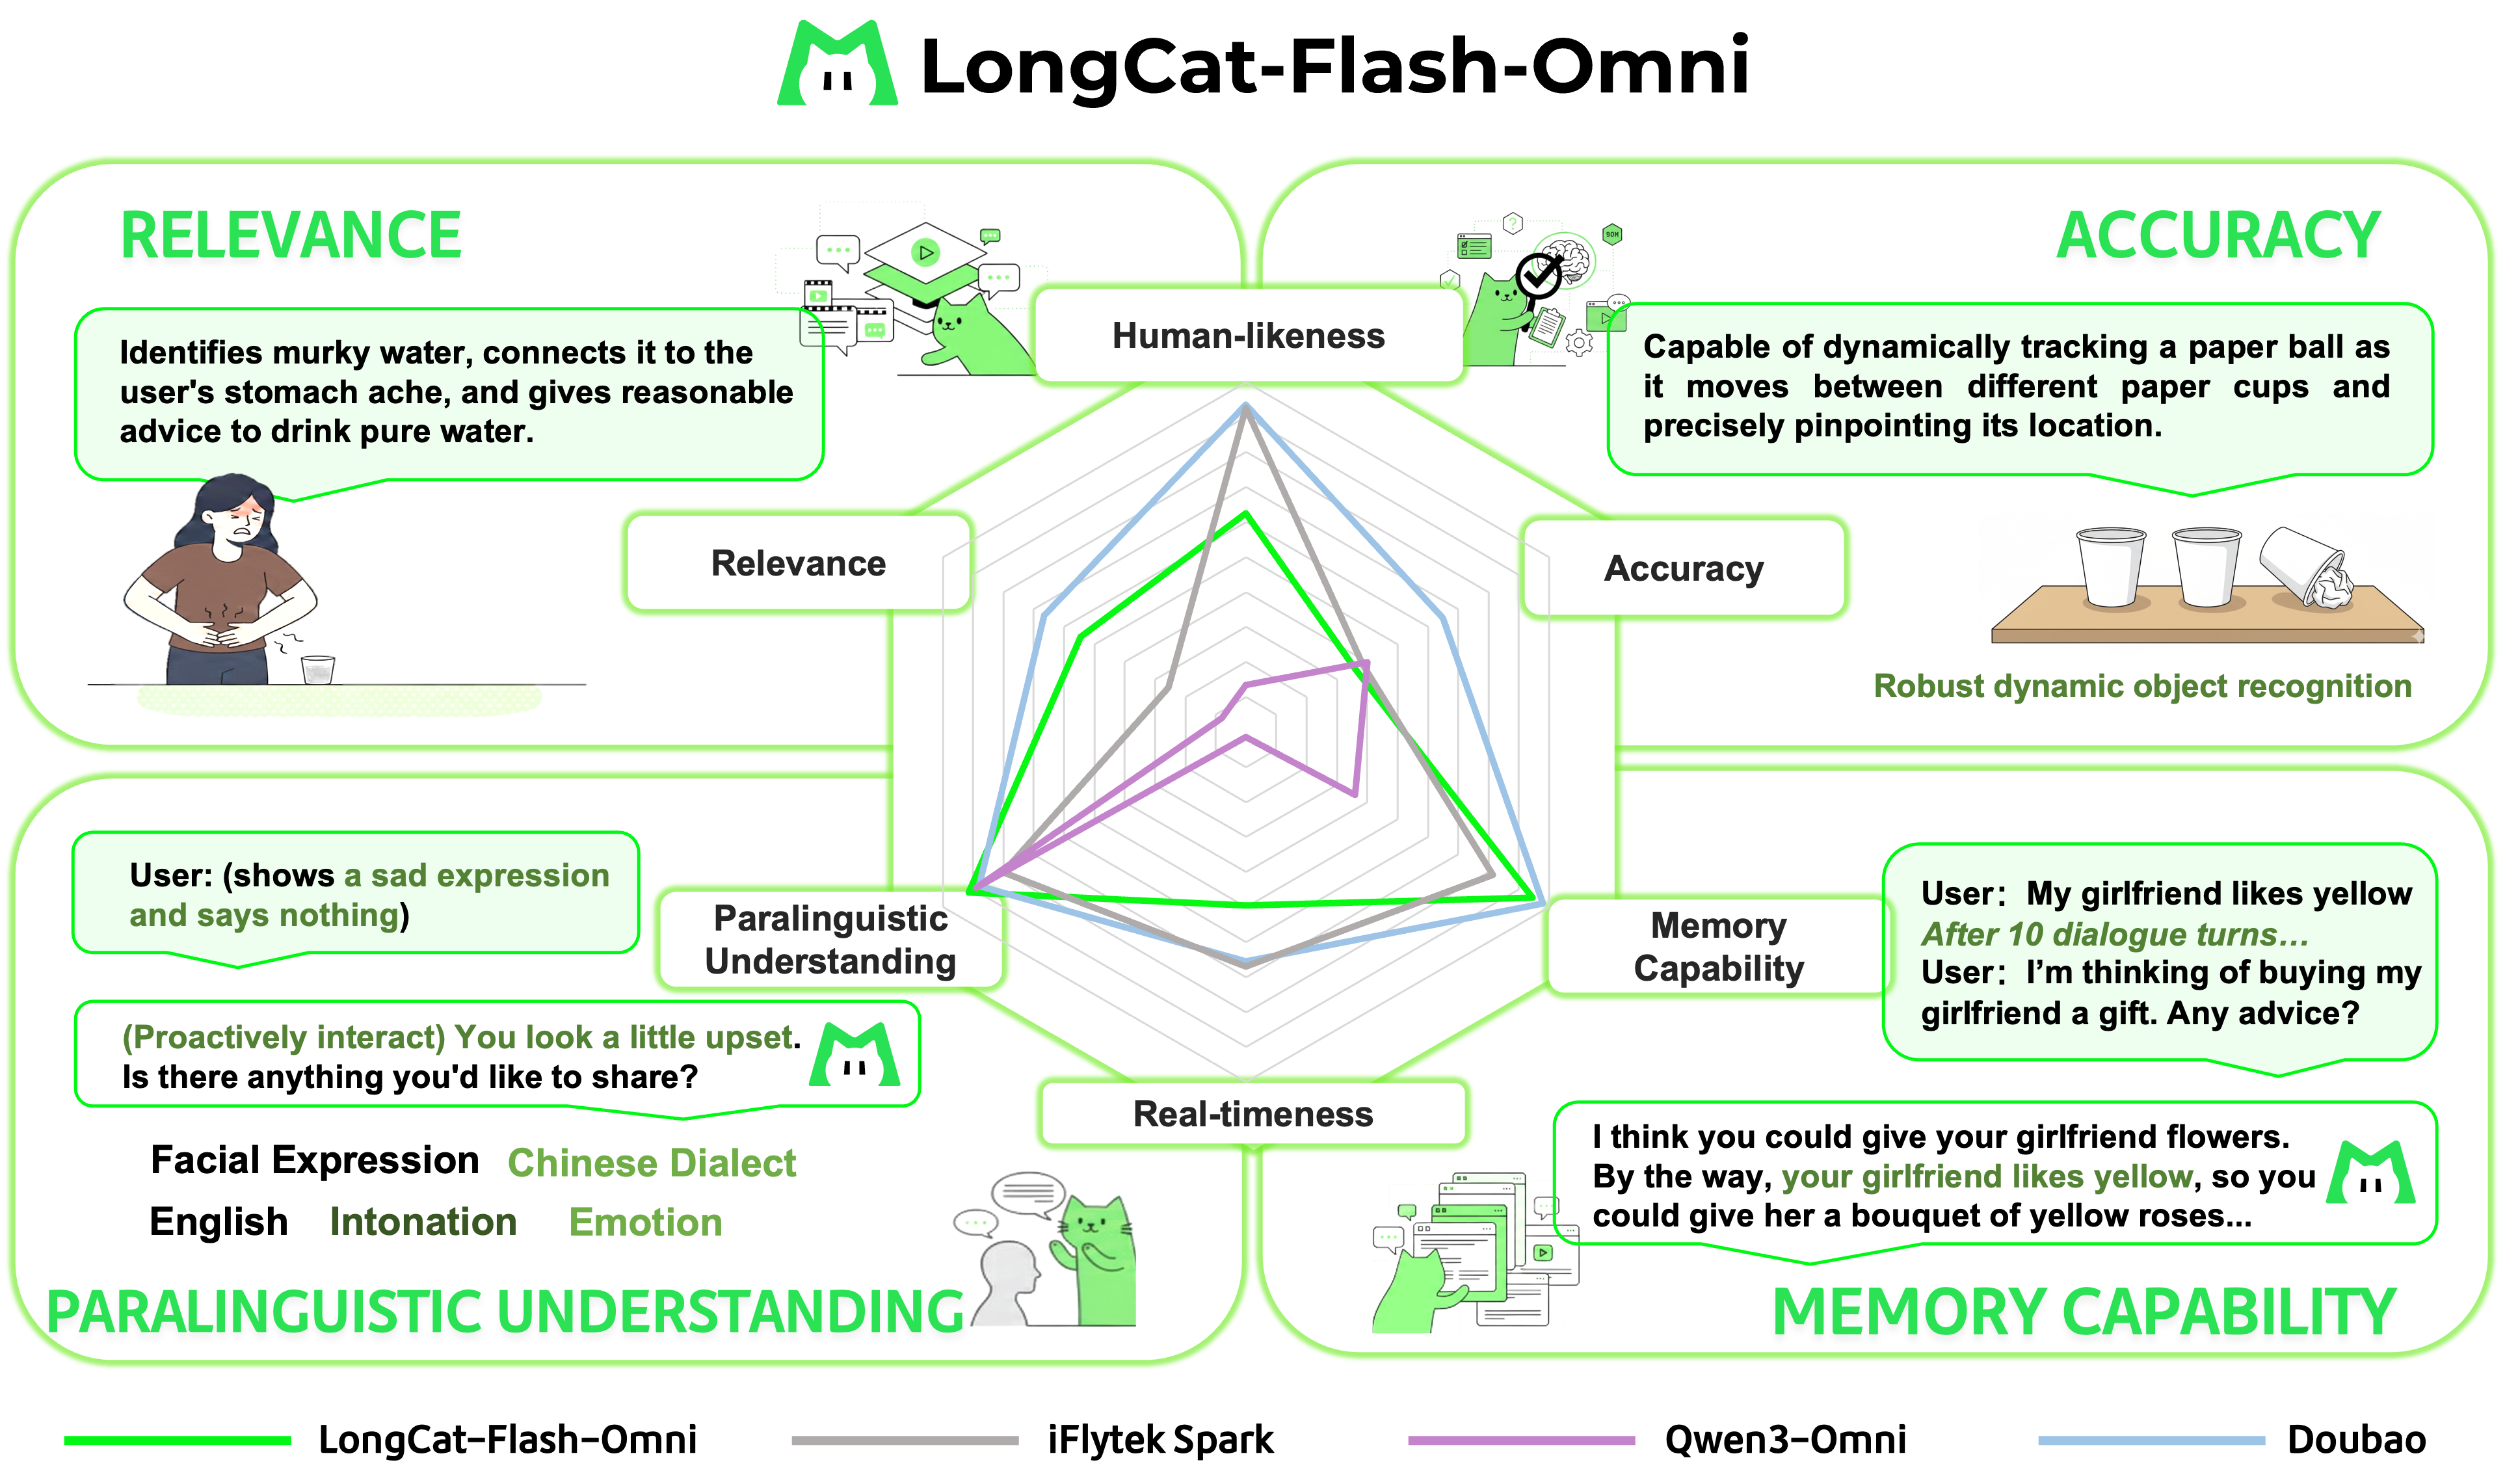
\includegraphics[width=0.9\textwidth]{figs/qualitative_analysis.png}
  \caption{Qualitative analysis of real-time audio-visual interaction.}
  \label{fig:qualitative_analysis}
\end{figure}

\begin{table}[htbp]
    \caption{Real-time audio-visual interaction evaluation.}
    \centering
    \resizebox{1.0\textwidth}{!}{
        \begin{tabular}{l|ccccccc|c}
            \toprule    
            Metrics & Doubao & GPT-4o & iFlytek Spark & StepFun & ChatGLM & Qwen2.5-Omni & Qwen3-Omni & \textbf{LongCat-Flash-Omni}\\
            \midrule
            Score & 1.92 & 1.79 & 1.25 & 1.22 & 0.99 & 0.96 & 0.81 & 1.37\\
            95\% CI & [1.85, 1.98] & [1.72, 1.85] & [1.18, 1.32] & [1.15, 1.28] & [0.93, 1.05] & [0.89, 1.02] & [0.75, 0.87] & [1.30, 1.44]\\

            \bottomrule
        \end{tabular}
    }
    \label{tab:real_time_interaction}
\end{table}

\begin{table}[htbp]
    \caption{Percentage of good cases in qualitative analysis.}
    \centering
    \resizebox{1.0\textwidth}{!}{
        \begin{tabular}{l|ccccccc|c}
            \toprule    
            Metrics & Doubao & GPT-4o & iFlytek Spark & StepFun & ChatGLM & Qwen2.5-Omni & Qwen3-Omni & \textbf{LongCat-Flash-Omni}\\
            \midrule
            Real-timeness & 65.5 & 71.5 & 67.0 & 18.0 & 3.0 & 4.0 & 1.5 & 49.5 \\
            Human-likeness & 93.5 & 69.0 & 92.5 & 70.5 & 76.5 & 59.0 & 13.5 & 62.5 \\
            Paralinguistic Understanding & 88.0 & 87.5 & 80.0 & 87.0 & 84.5 & 89.0 & 89.0 & 91.5 \\
            Relevance & 66.5 & 60.0 & 25.5 & 31.5 & 25.0 & 16.0 & 8.0 & 54.5 \\
            Accuracy & 65.0 & 55.0 & 38.5 & 42.5 & 33.5 & 35.5 & 40.0 & 36.0 \\
            Memory Capability & 98.0 & 98.0 & 81.5 & 92.5 & 83.0 & 64.0 & 36.0 & 94.5 \\
            \bottomrule
        \end{tabular}
    }
    \label{tab:percentage_of_qualitative}
\end{table}

% The data construction process involves 10 trained professional conversationalists who engaged in multi-turn dialog sessions (approximately 3 minutes each) with each model under evaluation. 
% These interactions are facilitated through real-time audio-visual interfaces on official APP or Web platforms provided by the model developers.
The data construction process involves 10 trained professional conversationalists who conducted multi-turn dialogue sessions (approximately three minutes each) with each model under evaluation. These interactions are carried out via real-time audio-visual interfaces on the official app or web platforms provided by the respective model developers.
% A total of 200 dialog sessions are collected for each model, including common real-life video call scenarios in four categories: problem solving, entertainment, self-improvement, and emotional support (50 samples per category).
A total of 200 dialogue sessions have been collected for each model, covering common real-world video call scenarios across four categories: problem solving, entertainment, self-improvement, and emotional support (50 samples per category).

% The assessment process combines quantitative user ratings with qualitative expert analysis.
% For quantitative ratings, 250 real users triple-annotate the full interaction videos, rating naturalness and fluency on a 4-point scale, where ``completely unnatural'' as 0, ``partially unnatural and affects interaction'' as 1, ``partially unnatural but does not affect interaction'' as 2, and ``completely natural and fluent'' as 3.
The assessment process combines quantitative user ratings with qualitative expert analysis. 
For quantitative evaluation, 250 real users independently triple-annotated the complete interaction videos, rating naturalness and fluency on a four-point scale: 
0 for \textit{completely unnatural}, 
1 for \textit{partially unnatural and affecting interaction}, 
2 for \textit{partially unnatural but not affecting interaction}, 
and 3 for \textit{completely natural and fluent}.
% For qualitative analysis, expert annotators perform a dimensional breakdown to identify specific issues impacting naturalness and fluency across seven key metrics, including interaction-level factors (real-timeness, human-likeness, paralinguistic-richness) and cognitive-level factors (relevance, accuracy, memory capability).
For qualitative analysis, expert annotators conduct a dimensional breakdown to identify specific factors affecting naturalness and fluency across six key factors, including \textit{real-timeness}, \textit{human-likeness}, \textit{paralinguistic understanding}, \textit{relevance}, \textit{accuracy} and \textit{memory capability}.
This approach provides comprehensive qualitative insights into each model's performance.

We compare LongCat-Flash-Omni with five audio-visual interaction products including Doubao\footnote{\url{https://www.doubao.com/chat/}, the evaluation period was August 11-15, 2025.}, GPT-4o\footnote{\url{https://chat.chatbot.app/?model=gpt-4o}, the evaluation period was August 18-22, 2025.}, iFlytek Spark\footnote{\url{https://xinghuo.xfyun.cn/desk}, the evaluation period was August 25-29, 2025.}, StepFun\footnote{\url{https://www.stepfun.com/chats/new}, the evaluation period was September 8-12, 2025.} and ChatGLM\footnote{\url{https://chat.z.ai/}, the evaluation period was September 1-5, 2025.}, as well as two open-source models Qwen2.5-Omni and Qwen3-Omni.

The quantitative ratings are presented in Table~\ref{tab:real_time_interaction}. 
LongCat-Flash-Omni achieves the third-highest score for naturalness and fluency in end-to-end interaction. 
%Among closed-source models, LongCat-Flash-Omni ranks behind Doubao and GPT-4o but outperforms iFlytek Spark and StepFun. 
Comparing with audio-visual interaction products, LongCat-Flash-Omni ranks behind Doubao and GPT-4o but outperforms iFlytek Spark and StepFun. 
Notably, LongCat-Flash-Omni demonstrates a substantial advantage over open-source alternatives, scoring 0.56 points higher than the current SOTA open-source model, Qwen3-omni.

We present the qualitative analysis results in Table~\ref{tab:percentage_of_qualitative}, together with some case study in Figure~\ref{fig:qualitative_analysis}.
LongCat-Flash-Omni excels in paralinguistic understanding, relevance, and memory capability, performing on par with top-tier models. 
Notably, LongCat-Flash-Omni actively interprets user emotions from both facial expressions and vocal cues, demonstrating its superior paralinguistic understanding. 
Regarding relevance, LongCat-Flash-Omni exhibits strong comprehension capabilities by closely tracking dialogue topics and generating highly correlated responses. 
This comprehension capability, combined with robust memory retention, enables LongCat-Flash-Omni to recall information from many turns earlier, resulting in more fluent and natural interactions. 
% However, LongCat-Flash-Omni still has some gaps compared to leading models in terms of real-timeness, human-likeness, and accuracy. 
% However, certain gaps remain compared with leading models, particularly in real-timeness, human-likeness, and accuracy. 
% Specifically, regarding real-timeness, the model demonstrates over-sensitivity to user pauses, frequently initiating responses prematurely and interrupting users mid-conversation. 
% In terms of human-likeness, the model occasionally produces pronunciation errors, stuttering, and robotic or electronic audio artifacts. 
% As for accuracy, while it demonstrates strong capability in recognizing dynamic objects, its recognition accuracy decreases when dealing with text and numbers. 
% Additionally, we've identified a tendency where the model is more inclined to agree with users' statements while neglecting visual recognition content. 
However, certain gaps remain compared with leading models, particularly in real-timeness, human-likeness, and accuracy. Specifically, in terms of real-timeness, our model tends to be overly sensitive to user pauses, often initiating responses prematurely and interrupting users mid-conversation. Regarding human-likeness, it occasionally exhibits pronunciation errors, stuttering, and robotic or electronic audio artifacts. In terms of accuracy, while our model shows strong capability in recognizing dynamic objects, its recognition performance declines when processing text and numerical information. Additionally, we observe a tendency for our model to over-agree with users’ statements while overlooking relevant visual content.
These aspects will be further optimized in the future work.



\section{Conclusion} % songxiang
\label{sec8:conclusion}

In this report, we present \longcat, a next-generation open-source omni-modal model that unifies robust offline multimodal understanding with real-time audio-visual interaction in a single, cohesive framework. \longcat demonstrates that large-scale models can effectively perceive, integrate, and generate across diverse modalities, including text, audio, image, and video, without sacrificing performance in any individual domain.

We address major challenges in building such a system: cross-modal heterogeneity, unified offline and streaming capabilities, and low-latency interaction. Through a carefully designed multi-stage early-fusion pretraining pipeline, \longcat achieves deeply integrated representations that enable synergistic multimodal reasoning while preserving unimodality strength. Our introduction of human-in-the-loop data construction and a 128K-token context window further enhances multi-turn dialogue, temporal reasoning, and memory capabilities in dynamic interactive scenarios.
On the architectural side, the adoption of the ScMoE backbone with zero-computation experts, together with lightweight modality encoders and decoder, allows the model to support real-time audio-visual interaction.

Extensive evaluations show that \longcat not only achieves state-of-the-art performance on omni-modal benchmarks such as Omni-Bench and WorldSense, but also matches or exceeds closed-source systems in key unimodal tasks, including image and video understanding as well as audio comprehension. Moreover, subjective assessments confirm the model’s ability to deliver natural, low-latency, high-quality interactive experiences, highlighting its potential as a foundation for next-generation human-AI interfaces.

Looking forward, \longcat lays a strong foundation for the continued evolution of omni-modal intelligence. Future work will focus on expanding the diversity and scale of training data, integrating an adaptive thinking mode, refining streaming and generation capabilities, and exploring richer forms of embodied and interactive intelligence. We believe that the release of \longcat will not only accelerate research on multimodal understanding and generation but also inspire new applications and paradigms for building human-centered, AGI-oriented systems.


\clearpage

\section{Contributions}

The list of authors is in alphabetical order. Names marked with an asterisk ($\ast$) indicate people who have left our team.

\begin{CJK}{UTF8}{gkai}
\renewcommand{\arraystretch}{1.2}
\begin{tabular}{p{0.25\textwidth}p{0.25\textwidth}p{0.25\textwidth}p{0.25\textwidth}}
% Bairui Wang & Jian Yang & Senbin Yang & Xuezhi Cao \\
% Bayan & Jiaxing Liu & Shanbo Xu & Xunliang Cai \\
% Bin Xiao & Jing Huang & Shanglin Lei & Yang Yang \\
% Bo Zhang$^\ast$ & Jingang Wang & Shengze Ye & Yanli Tan \\
% Bolin Rong & Jinrui Ding & Shimin Chen & Yao Yao \\
% Borun Chen & Juchao Jiang & Shuaiqi Chen & Yerui Sun \\
% Chang Wan & Jun Kuang & Shuo Li & Yi Chen \\
% Chao Zhang & Jun Wang & Siqi Yang & Yifan Lu \\
% Chen Chen (陈琛) & Junhui Mei & Siyu Ren & Yin Gong \\
% Chen Chen (陈晨) & Ke Ding & Siyu Xu & Yining Zhang \\
% Chen Huang & Kefeng Zhang & Song Li & Yitian Chen \\
% Chengxu Yang & Lei Chen & Songxiang Liu & Yiyang Gan \\
% Chengzuo Yang & Liang Shi & Tianhao Bai & Yuchen Tang \\
% Dandan Peng & Limeng Qiao & Tianye Dai & Yuchen Xie \\
% Delian Ruan & Liming Zheng & Wei Hong & Yueqian Wang \\
% Detai Xin & Lin Ma & Wei Wang & Yuewen Zheng \\
% Disong Wang & Liuyang Guo & Weixiao Zhao & Yufei Zhang \\
% Dongchao Yang & Liya Ma & Wengang Cao & Yufeng Zhong \\
% Fanfan Liu & Luying Sun & Wenlong He & Yulei Qian \\
% Fengjiao Chen & Man Gao & Wenlong Zhu & Yuqi Peng \\
% Fengyu Yang & Mengshen Zhu & Xi Nan & Yuwei Jiang \\
% Gan Dong & Miao Cao & Xi Su & Zeyang Hu \\
% Gang Huang & Minliang Lin & Xiaohan Zhao & Zheng Zhang \\
% Gang Xu & Nuo Xu & Xiaohao Wang & Zhengkun Tian$^\ast$ \\
% Guanglu Wan & Peng Shi & Xiaoyu Li & Zhiqing Hong \\
% Guoqiang Tan & Qi Zhang & Xiaoyu Wang & Zhixiong Zeng \\
% Guoqiao Yu & Qian Fang & Xiaoyu Zhao & Zhuqi Mi \\
% Haibo Qiu & Qian Wang & Xin Chen & Ziran Li \\
% Hao Lu & Qian Yang & Xin Pan & Ziwen Wang \\
% Hongbo Liu & Quanxiu Wang & Xiusong Sun & Ziyi Zhao \\
% Hongyu Xiang & Rongxiang Weng & Xu Xiang & Ziyuan Zhuang \\
% Jiaheng Wu & Ruoxuan Liang & Xudong Xing & Zizhe Zhao \\

% Bairui Wang & Jian Yang & Senbin Yang & Xuezhi Cao \\
% Bayan & Jiaxing Liu & Shanbo Xu & Xunliang Cai \\
% Bin Xiao & Jing Huang & Shanglin Lei & Yang Yang \\
% Bo Zhang * & Jingang Wang & Shengze Ye & Yanli Tan \\
% Bolin Rong & Jinrui Ding & Shimin Chen & Yao Yao \\
% Borun Chen & Juchao Jiang & Shuaiqi Chen & Yerui Sun \\
% Chang Wan & Jun Kuang & Shujie Hu & Yi Chen \\
% Chao Zhang & Jun Wang & Shuo Li & Yifan Lu \\
% Chen Chen (陈晨) & Junhui Mei & Siqi Yang & Yin Gong \\
% Chen Chen (陈琛) & Ke Ding & Siyu Ren & Yining Zhang \\
% Chen Huang & Kefeng Zhang & Siyu Xu & Yitian Chen \\
% Chengxu Yang & Lei Chen & Song Li & Yiyang Gan \\
% Chengzuo Yang & Liang Shi & Songxiang Liu & Yuchen Tang \\
% Cong Han * & Limeng Qiao & Tianhao Bai & Yuchen Xie \\
% Dandan Peng & Liming Zheng & Tianye Dai & Yueqian Wang \\
% Delian Ruan & Lin Ma & Wei Hong & Yuewen Zheng \\
% Detai Xin & Liuyang Guo & Wei Wang & Yufei Zhang \\
% Disong Wang & Liya Ma & Weixiao Zhao & Yufeng Zhong \\
% Dongchao Yang & Luying Sun & Wengang Cao & Yulei Qian \\
% Fanfan Liu & Man Gao & Wenlong He & Yuqi Peng \\
% Fengjiao Chen & Mengshen Zhu & Wenlong Zhu & Yuwei Jiang \\
% Fengyu Yang & Miao Cao & Xi Nan & Zeyang Hu \\
% Gan Dong & Minliang Lin & Xi Su & Zheng Zhang \\
% Gang Huang & Nuo Xu & Xiaohan Zhao & Zhengkun Tian * \\
% Gang Xu & Peng Shi & Xiaohao Wang & Zhiqing Hong \\
% Guanglu Wan & Qi Zhang & Xiaoyu Li & Zhixiong Zeng \\
% Guoqiang Tan & Qian Fang & Xiaoyu Wang & Zhuqi Mi \\
% Guoqiao Yu & Qian Wang & Xiaoyu Zhao & Ziran Li \\
% Haibo Qiu & Qian Yang & Xin Chen & Ziwen Wang \\
% Hao Lu & Quanxiu Wang & Xin Pan & Ziyi Zhao \\
% Hongbo Liu & Rongxiang Weng & Xiusong Sun & Ziyuan Zhuang \\
% Hongyu Xiang & Rongxin Guo * & Xu Xiang & Zizhe Zhao \\
% Jiaheng Wu & Ruoxuan Liang & Xudong Xing &  \\
Bairui Wang & Jian Yang & Senbin Yang & Xuezhi Cao \\
Bayan & Jiaxing Liu & Shanbo Xu & Xunliang Cai \\
Bin Xiao & Jing Huang & Shanglin Lei & Yang Yang \\
Bo Zhang * & Jingang Wang & Shengze Ye & Yanli Tan \\
Bolin Rong & Jinrui Ding & Shimin Chen & Yao Yao \\
Borun Chen & Juchao Jiang & Shuaiqi Chen & Yerui Sun \\
Chang Wan & Jun Kuang & Shujie Hu & Yi Chen \\
Chao Zhang & Jun Wang & Shuo Li & Yifan Lu \\
Chen Chen (陈晨) & Junhui Mei & Siqi Yang & Yin Gong \\
Chen Chen (陈琛) & Ke Ding & Siyu Ren & Yining Zhang \\
Chen Huang & Kefeng Zhang & Siyu Xu & Yitian Chen \\
Chengxu Yang & Lei Chen & Song Li & Yiyang Gan \\
Chengzuo Yang & Liang Shi & Songxiang Liu & Yuchen Tang \\
Cong Han * & Limeng Qiao & Tianhao Bai & Yuchen Xie \\
Dandan Peng & Liming Zheng & Tianye Dai & Yueqian Wang \\
Delian Ruan & Lin Ma & Wei Hong & Yuewen Zheng \\
Detai Xin & Liuyang Guo & Wei Wang & Yufei Zhang \\
Disong Wang & Liya Ma & Weixiao Zhao & Yufeng Zhong \\
Dongchao Yang & Luying Sun & Wengang Cao & Yulei Qian \\
Fanfan Liu & Man Gao & Wenlong He & Yuqi Peng \\
Fengjiao Chen & Mengshen Zhu & Wenlong Zhu & Yuqian Li \\
Fengyu Yang & Miao Cao & Xi Nan & Yuwei Jiang \\
Gan Dong & Minliang Lin & Xi Su & Zeyang Hu \\
Gang Huang & Nuo Xu & Xiaohan Zhao & Zheng Zhang \\
Gang Xu & Peng Shi & Xiaohao Wang & Zhengkun Tian * \\
Guanglu Wan & Qi Zhang & Xiaoyu Li & Zhiqing Hong \\
Guoqiang Tan & Qian Fang & Xiaoyu Wang & Zhixiong Zeng \\
Guoqiao Yu & Qian Wang & Xiaoyu Zhao & Zhuqi Mi \\
Haibo Qiu & Qian Yang & Xin Chen & Ziran Li \\
Hao Lu & Quanxiu Wang & Xin Pan & Ziwen Wang \\
Hongbo Liu & Rongxiang Weng & Xiusong Sun & Ziyi Zhao \\
Hongyu Xiang & Rongxin Guo * & Xu Xiang & Ziyuan Zhuang \\
Jiaheng Wu & Ruoxuan Liang & Xudong Xing & Zizhe Zhao \\
\end{tabular}
\end{CJK}

\clearpage

\bibliographystyle{unsrtnat}
\bibliography{references}  

\clearpage

% \appendix
% \section{Appendix}\label{appendix}


\end{document}

 